\documentclass[letterpaper,10pt,titlepage]{custbook}
%
\pagestyle{headings}
%
\usepackage{amsmath}
\usepackage{amsfonts}
\usepackage{amssymb}
\usepackage[ansinew]{inputenc}
\usepackage[OT1]{fontenc}
\usepackage{graphicx}
\usepackage{longtable}
\usepackage{makeidx}
%
%Packages that must go in the document preamble.
\makeindex
%
%Define certain conspicuous global constants.
\newcommand{\productbasenamelong}{Embedded Tool Set}
\newcommand{\productbasenameshort}{EMTS}
\newcommand{\productversion}{0.1.0}
\newcommand{\productname}{\productbasenameshort{}-\productversion}
%
%Shared mathematical definitions
% $Header: /home/dashley/cvsrep/uculib01/uculib01/doc/manual/comps/workmdef.tex,v 1.2 2007/08/30 14:25:20 dtashley Exp $
%
%%Sets of real numbers.
\newcommand{\vworkrealset}{{\mathbb{R}}}
\newcommand{\vworkrealsetnonneg}{{\mathbb{R}^+}}
%
%%Sets of integers.
\newcommand{\vworkintset}{{\mathbb{Z}}}
\newcommand{\vworkintsetnonneg}{{\mathbb{Z}^+}}
\newcommand{\vworkintsetpos}{{\mathbb{N}}}
%
%%Sets of rational numbers.
\newcommand{\vworkratset}{{\mathbb{Q}}}
\newcommand{\vworkratsetnonneg}{{\mathbb{Q}^+}}
%
%%Sets of irrational numbers.
\newcommand{\vworkirratset}{{\mathbb{error}}}
\newcommand{\vworkirratsetnonneg}{{\mathbb{error}^+}}
%
%%"Divides" and "Not Divides".  Am not able to find quite
%%the right symbol for "Not Divides" at this time.
\newcommand{\vworkdivides}{\mid}
\newcommand{\vworknotdivides}{\hspace{-0.125em}\not\hspace{0.245em}\mid\hspace{0.135em}}
%%
%%The implication operator, which may change throughout the work.  Both a horizontal
%%and vertical form are defined.
\newcommand{\vworkhimp}{\to}
\newcommand{\vworkvimp}{\downarrow}
%%
%%The symbol for logical equivalence.  There are three forms defined, the standard,
%%the long, and the short, which may be identical.
\newcommand{\vworkequiv}{\leftrightarrow}
\newcommand{\vworkshortequiv}{\leftrightarrow}
\newcommand{\vworklongequiv}{\longleftrightarrow}
\newcommand{\vworkvertequiv}{\updownarrow}

%$Log: workmdef.tex,v $
%Revision 1.2  2007/08/30 14:25:20  dtashley
%Edits.
%
%Revision 1.1  2007/08/30 14:24:32  dtashley
%Initial checkin.
%
%End of $RCSfile: workmdef.tex,v $.
%
%Hyphenation exceptions
%$Header: svn://localhost/dtapublic/pubs/books/ucbka/trunk/volshare/workhxcp.tex 274 2019-08-11 21:43:05Z dashley $
%
%This file contains hyphenation exceptions for work.
\hyphenation{EEPROM}
\hyphenation{MATLAB}
\hyphenation{SIMULINK}
\hyphenation{UPPAAL}
%
%End of file WORKHXCP.TEX

%
%New environments, etc.
\input{comps/worknenv}
%
\begin{document}
%
%Index "see" definitions
% $Header: /home/dashley/cvsrep/e3ft_gpl01/e3ft_gpl01/webprojs/pamc/gen_a/docs/manual/man_a/comps/workidxs.tex,v 1.2 2007/06/04 00:26:38 dashley Exp $
%
% This file contains the "see" definitions for the index.  It is easier to
% keep all of these definitions in one place.
%
%%%%%%%%%%%%%%%%%%%%%%%%%%%%%%%%%%%%%%%%%%%%%%%%%%%%%%%%%%%%%%%%%%%%%%%%%%%%%
% A
%
%%%%%%%%%%%%%%%%%%%%%%%%%%%%%%%%%%%%%%%%%%%%%%%%%%%%%%%%%%%%%%%%%%%%%%%%%%%%%
% B
%
%%%%%%%%%%%%%%%%%%%%%%%%%%%%%%%%%%%%%%%%%%%%%%%%%%%%%%%%%%%%%%%%%%%%%%%%%%%%%
% C
%
%%%%%%%%%%%%%%%%%%%%%%%%%%%%%%%%%%%%%%%%%%%%%%%%%%%%%%%%%%%%%%%%%%%%%%%%%%%%%
% D
\index{David T. Ashley|see{Ashley, David T.}}
%
%%%%%%%%%%%%%%%%%%%%%%%%%%%%%%%%%%%%%%%%%%%%%%%%%%%%%%%%%%%%%%%%%%%%%%%%%%%%%
% F
%
%%%%%%%%%%%%%%%%%%%%%%%%%%%%%%%%%%%%%%%%%%%%%%%%%%%%%%%%%%%%%%%%%%%%%%%%%%%%%
% F
%
%%%%%%%%%%%%%%%%%%%%%%%%%%%%%%%%%%%%%%%%%%%%%%%%%%%%%%%%%%%%%%%%%%%%%%%%%%%%%
% G
\index{g.c.d.|see{greatest common divisor}}
%
%%%%%%%%%%%%%%%%%%%%%%%%%%%%%%%%%%%%%%%%%%%%%%%%%%%%%%%%%%%%%%%%%%%%%%%%%%%%%
% H
%
%%%%%%%%%%%%%%%%%%%%%%%%%%%%%%%%%%%%%%%%%%%%%%%%%%%%%%%%%%%%%%%%%%%%%%%%%%%%%
% I
%
%%%%%%%%%%%%%%%%%%%%%%%%%%%%%%%%%%%%%%%%%%%%%%%%%%%%%%%%%%%%%%%%%%%%%%%%%%%%%
% J
%
%%%%%%%%%%%%%%%%%%%%%%%%%%%%%%%%%%%%%%%%%%%%%%%%%%%%%%%%%%%%%%%%%%%%%%%%%%%%%
% K
%
%%%%%%%%%%%%%%%%%%%%%%%%%%%%%%%%%%%%%%%%%%%%%%%%%%%%%%%%%%%%%%%%%%%%%%%%%%%%%
% L
%
%%%%%%%%%%%%%%%%%%%%%%%%%%%%%%%%%%%%%%%%%%%%%%%%%%%%%%%%%%%%%%%%%%%%%%%%%%%%%
% M
%
%%%%%%%%%%%%%%%%%%%%%%%%%%%%%%%%%%%%%%%%%%%%%%%%%%%%%%%%%%%%%%%%%%%%%%%%%%%%%
% N
%
%%%%%%%%%%%%%%%%%%%%%%%%%%%%%%%%%%%%%%%%%%%%%%%%%%%%%%%%%%%%%%%%%%%%%%%%%%%%%
% O
%
%%%%%%%%%%%%%%%%%%%%%%%%%%%%%%%%%%%%%%%%%%%%%%%%%%%%%%%%%%%%%%%%%%%%%%%%%%%%%
% P
%
%%%%%%%%%%%%%%%%%%%%%%%%%%%%%%%%%%%%%%%%%%%%%%%%%%%%%%%%%%%%%%%%%%%%%%%%%%%%%
% R
%
%%%%%%%%%%%%%%%%%%%%%%%%%%%%%%%%%%%%%%%%%%%%%%%%%%%%%%%%%%%%%%%%%%%%%%%%%%%%%
% S
%
%%%%%%%%%%%%%%%%%%%%%%%%%%%%%%%%%%%%%%%%%%%%%%%%%%%%%%%%%%%%%%%%%%%%%%%%%%%%%
% T
%
%%%%%%%%%%%%%%%%%%%%%%%%%%%%%%%%%%%%%%%%%%%%%%%%%%%%%%%%%%%%%%%%%%%%%%%%%%%%%
% U
%
%%%%%%%%%%%%%%%%%%%%%%%%%%%%%%%%%%%%%%%%%%%%%%%%%%%%%%%%%%%%%%%%%%%%%%%%%%%%%
% Y
%
%%%%%%%%%%%%%%%%%%%%%%%%%%%%%%%%%%%%%%%%%%%%%%%%%%%%%%%%%%%%%%%%%%%%%%%%%%%%%
%$Log: workidxs.tex,v $
%Revision 1.2  2007/06/04 00:26:38  dashley
%Edits.
%
%Revision 1.1  2007/04/10 23:41:25  dashley
%Initial checkin.
%
%End of $RCSfile: workidxs.tex,v $.

%
%Title page(s)
%$Header: svn://localhost/dtapublic/pubs/books/ucbka/trunk/volshare/workttla.tex 274 2019-08-11 21:43:05Z dashley $

\thispagestyle{empty}

\begin{flushright}
%\vspace{20cm}
\huge\bfseries
A Practitioner's Guide To The
Design And Development Of
Small Microcontroller Software
\end{flushright}
\vspace{0.0cm}
\noindent\rule{\textwidth}{2pt}
\begin{flushright}
\huge\bfseries
\curvoltitlepageprefix{}\curvolroman{}\curvoltitlepagesep{}\curvoltitle{}
\end{flushright}
\vfill
\begin{flushright}
\begin{small}
%$Header: svn://localhost/dtapublic/pubs/books/ucbka/trunk/volshare/workalst.tex 274 2019-08-11 21:43:05Z dashley $
%
%This file contains the list of authors for the entire work, as it should be inserted on title
%pages.

David T. Ashley

%
%End of file WORKALST.TEX

\end{small}
\end{flushright}
\vspace{0.2cm}
\begin{flushright}
\begin{small}
Volume compiled from \LaTeX{} source code on \today .  
This document and supporting materials
are maintained on the Web at \texttt{http://esrg.sourceforge.net}.
\end{small}
\end{flushright}

\pagebreak
\thispagestyle{empty}
\begin{small}
  \noindent Copyright \copyright 1999--2003 David T. Ashley.
  Licensed under \emph{The Academic Free License version 2.0}.
  For convenience, the license is reprinted in the preface.
  In order to comply with \emph{Paragraph 3} of the license,
  the \LaTeX{} source code and graphics for this book have
  been made available at \texttt{http://esrg.sourceforge.net}.
\end{small}

\vfill

%Version control information for this file.
\noindent\begin{minipage}{\textwidth}
\noindent\rule[-0.25in]{\textwidth}{1pt}
\begin{tiny}
\begin{verbatim}
$HeadURL: svn://localhost/dtapublic/pubs/books/ucbka/trunk/volshare/workttla.tex $
$Revision: 274 $
$Date: 2019-08-11 17:43:05 -0400 (Sun, 11 Aug 2019) $
$Author: dashley $
\end{verbatim}
\end{tiny}
\noindent\rule[0.25in]{\textwidth}{1pt}
\end{minipage}
%
%End of WORKTTLA.TEX

%
%Declare this as frontmatter, the front portion before the meat
%of the book.
\frontmatter{}
%
%Preface
%$Header: /home/dashley/cvsrep/e3ft_gpl01/e3ft_gpl01/webprojs/pamc/gen_a/docs/manual/man_a/comps/workprfa.tex,v 1.9 2009/10/31 19:02:03 dashley Exp $
\chapter{Preface}

The product described in this document, 
\emph{\productbasename{} Version \productversion{}}
(also called \emph{\productbasename{}-\productversion{}}),
is a free open-source server-based collaboration solution for 
product development.  

\emph{\productbasename{}-\productversion{}}
is a recipe for transforming 
a \emph{*nix} server into a 
product development collaboration platform.
\emph{\productbasename{}-\productversion{}} does provide
original content, but a large part of the functionality of
\emph{\productbasename{}-\productversion{}} is built
on other open-source products such as 
\emph{*nix}, \emph{cvs}, \emph{svn}, \emph{PHP}, 
\emph{MySQL}, and \emph{putty}.

\emph{\productbasename{}-\productversion{}} provides the
following functionality:

\begin{itemize}
\item Secure access to \emph{*nix} shell accounts and
      SFTP, secured by \emph{SSH} and \emph{CryptoCard} tokens.
\item Personal web space, secured by \emph{CryptoCard} tokens
      used in conjunction with an \emph{Apache} authentication
      module.
\item Version control, implemented via 
      \emph{cvs} and \emph{svn} and secured
      via secure port forwarding and
      \emph{putty}.
\item A general web database platform.

   \begin{itemize}
   \item The platform is secured with \emph{CryptoCard} tokens,
         static passwords, IP restrictions, and \emph{https}.
   \item The platform as installed provides substantial
         useful functionality, including:

         \begin{itemize}
         \item User authentication and management.
         \item E-mail notifications.
         \item Employee time tracking and hours reporting.
         \item Viewing of version control archives.
         \item Document management.
         \item Software defect tracking.
         \item Automatic database maintenance.
         \end{itemize}

   \item The platform is designed to be easily extended by allowing
         the addition of custom applications that operate in the same
         authentication framework.
   \end{itemize}
\end{itemize}

\emph{\productbasename{}-\productversion{}} can be used as-is, or individual
components can be harvested for use in other applications.  For example,
the compiled \emph{C} program and \emph{PHP} functions that allow \emph{CryptoCard} tokens
to be used from \emph{PHP} may be useful in other applications.

\emph{\textbf{Part I: General Information}} provides introductory
and general information about the product.

\emph{\textbf{Part II: Technical Information}} provides a detailed
technical description of the product and its theory of operation.

\emph{\textbf{Part III: Installation and Maintenance}} provides an installation
guide for the product and instructions for maintaining the product.  
\emph{\productbasename{}-\productversion{}}
is designed for use only on \emph{*nix} platforms.

\emph{\textbf{Part IV: User Information}} provides a 
non-technical user manual for the product.

\emph{\textbf{Part V: Procedures and Checklists}} provides a 
set of procedures and checklists to accomplish tasks where the
procedure or checklist didn't fit well into any other part of this
document.

\emph{\textbf{Part VI: Appendices, Bibliography, and Index}} provides
glossaries, references, and an index.
Individuals, products, companies, websites, and Internet newsgroups
are cited in the same framework
as traditional references in order to provide the reader with more
resources to obtain information.

The \emph{\productbasename{}-\productversion{}} software and all
associated materials are provided under open-source licenses; so all source
code is available and the product can be modified and/or distributed with
minimal restrictions.

Please feel free to contact me at \texttt{dashley@gmail.com} with
any suggestions for the \emph{\productbasename{}-\productversion{}}
product or associated documentation.  If you require
assistance with the product, please refer to
\S{}\ref{ciov0:soas0} (p. \pageref{ciov0:soas0}).

I hope that this product is useful to you and that you
find it easy to install, use, maintain, and modify.

\vspace*{0.5in}

\noindent{}\hspace*{75mm}David T. Ashley                \\
           \hspace*{75mm}Marshall, Michigan, USA        \\
           \hspace*{75mm}November, 2009                 \\

%%%%%%%%%%%%%%%%%%%%%%%%%%%%%%%%%%%%%%%%%%%%%%%%%%%%%%%%%%%%%%%%%%%%%%%%%%

\noindent\begin{figure}[!b]
\noindent\rule[-0.25in]{\textwidth}{1pt}
\begin{tiny}
\begin{verbatim}
$RCSfile: workprfa.tex,v $
$Source: /home/dashley/cvsrep/e3ft_gpl01/e3ft_gpl01/webprojs/pamc/gen_a/docs/manual/man_a/comps/workprfa.tex,v $
$Revision: 1.9 $
$Author: dashley $
$Date: 2009/10/31 19:02:03 $
\end{verbatim}
\end{tiny}
\noindent\rule[0.25in]{\textwidth}{1pt}
\end{figure}

%$Log: workprfa.tex,v $
%Revision 1.9  2009/10/31 19:02:03  dashley
%Edits.
%
%Revision 1.8  2009/10/29 17:46:12  dashley
%Edits.
%
%Revision 1.7  2009/10/29 04:52:52  dashley
%Edits.
%
%Revision 1.6  2007/07/11 01:36:52  dashley
%Edits.
%
%Revision 1.5  2007/06/06 00:32:07  dashley
%Edits.
%
%Revision 1.4  2007/06/05 15:47:12  dashley
%Structural edits.
%
%Revision 1.3  2007/06/04 06:26:36  dashley
%Edits.
%
%Revision 1.2  2007/06/03 04:57:47  dashley
%Checkin to be sure that changes wrapped up in weekly TAR.GZ file.
%
%Revision 1.1  2007/04/10 23:44:47  dashley
%Initial checkin.
%
%End of $RCSfile: workprfa.tex,v $.

%
%Acknowledgements
%$Header: /home/dashley/cvsrep/e3ft_gpl01/e3ft_gpl01/webprojs/pamc/gen_a/docs/manual/man_a/comps/workacks.tex,v 1.3 2009/10/31 20:02:15 dashley Exp $
\chapter{Acknowledgements}

I'm vary grateful to my employer, Cequent Electrical 
Products \index{Cequent Electrical Products}\cite{bibref:c:cequentelectricalproducts}, 
for allowing me
to pursue certain aspects of this effort in the workplace, and for allowing
me to use corporate needs as a testbed for potential solutions.
I'm especially grateful to Marcia Albright\index{Albright, Marcia} \cite{bibref:i:marciaalbright}
and Doug Motts\index{Motts, Doug} \cite{bibref:i:dougmotts}

A working two-factor authentication solution would not have been
possible without support and assistance from
CryptoCard Corporation\index{CryptoCard Corporation} \cite{bibref:c:cryptocardcorporation}\@.
I'm especially grateful to Bill LaHam\index{LaHam, Bill} \cite{bibref:i:billlaham}
and John Cebasek\index{Cebasek, John} \cite{bibref:i:johncebasek}.


%%%%%%%%%%%%%%%%%%%%%%%%%%%%%%%%%%%%%%%%%%%%%%%%%%%%%%%%%%%%%%%%%%%%%%%%%%%%%%%
\begin{figure}[b]
\noindent\rule[-0.25in]{\textwidth}{1pt}
\begin{tiny}
\begin{verbatim}
$RCSfile: workacks.tex,v $
$Source: /home/dashley/cvsrep/e3ft_gpl01/e3ft_gpl01/webprojs/pamc/gen_a/docs/manual/man_a/comps/workacks.tex,v $
$Revision: 1.3 $
$Author: dashley $
$Date: 2009/10/31 20:02:15 $
\end{verbatim}
\end{tiny}
\noindent\rule[0.25in]{\textwidth}{1pt}
\end{figure}

%$Log: workacks.tex,v $
%Revision 1.3  2009/10/31 20:02:15  dashley
%Edits.
%
%Revision 1.2  2007/06/03 04:57:47  dashley
%Checkin to be sure that changes wrapped up in weekly TAR.GZ file.
%
%Revision 1.1  2007/04/10 23:46:08  dashley
%Initial checkin.
%
%End of $RCSfile: workacks.tex,v $.

%
%Table of contents
\tableofcontents
%
%List of tables
\listoftables
%
%List of figures
\listoffigures
%
%List of procedures and checklists
%\listofprocchklsts
%
%Everything after this is the main matter, the "meat"
%of the book.
\mainmatter{}
%
%Part: General Information
\part{General Information}

%Chapter: Introduction and Overview
%%%%%%%%%%%%%%%%%%%%%%%%%%%%%%%%%%%%%%%%%%%%%%%%%%%%%%%%%%%%%%%%%%%%%%%%%%%%%%%%%%%%%%%%%%%%%%%%%%%%
\chapter{Introduction and Overview}

\label{ciov0}

%%%%%%%%%%%%%%%%%%%%%%%%%%%%%%%%%%%%%%%%%%%%%%%%%%%%%%%%%%%%%%%%%%%%%%%%%%%%%%%%%%%%%%%%%%%%%%%%%%%%
%%%%%%%%%%%%%%%%%%%%%%%%%%%%%%%%%%%%%%%%%%%%%%%%%%%%%%%%%%%%%%%%%%%%%%%%%%%%%%%%%%%%%%%%%%%%%%%%%%%%
%%%%%%%%%%%%%%%%%%%%%%%%%%%%%%%%%%%%%%%%%%%%%%%%%%%%%%%%%%%%%%%%%%%%%%%%%%%%%%%%%%%%%%%%%%%%%%%%%%%%
\section{Introduction and Overview}
\label{ciov2:siov0}

TBD.

%%%%%%%%%%%%%%%%%%%%%%%%%%%%%%%%%%%%%%%%%%%%%%%%%%%%%%%%%%%%%%%%%%%%%%%%%%%%%%%%%%%%%%%%%%%%%%%%%%%%
%%%%%%%%%%%%%%%%%%%%%%%%%%%%%%%%%%%%%%%%%%%%%%%%%%%%%%%%%%%%%%%%%%%%%%%%%%%%%%%%%%%%%%%%%%%%%%%%%%%%
%%%%%%%%%%%%%%%%%%%%%%%%%%%%%%%%%%%%%%%%%%%%%%%%%%%%%%%%%%%%%%%%%%%%%%%%%%%%%%%%%%%%%%%%%%%%%%%%%%%%
\section{License}\index{license}
\label{ciov2:slic0}

This document, all computer and paper files and records used to create and
distribute this document, the software described by this document, and all computer
and paper files and records used to create and distribute the software described by
this document, are provided under \index{MIT license@\emph{The MIT License}}\emph{The MIT License},
reproduced immediately below.\\

\begin{small}
\noindent{}\emph{Copyright \copyright 2020 David T. Ashley}\\\\
\noindent{}\emph{Permission is hereby granted, free of charge, to any person obtaining a copy
of this software source code and associated documentation files (the
``Software''), to deal in the Software without restriction, including without
limitation the rights to use, copy, modify, merge, publish, distribute,
sublicense, and/or sell copies of the Software, and to permit persons to whom
the Software is furnished to do so, subject to the following conditions:}

\begin{itemize}
\item \emph{The above copyright notice and this permission notice shall be included in
      all copies or substantial portions of the Software.}
\item \emph{THE SOFTWARE IS PROVIDED ``AS IS'', WITHOUT WARRANTY OF ANY KIND, EXPRESS OR
      IMPLIED, INCLUDING BUT NOT LIMITED TO THE WARRANTIES OF MERCHANTABILITY,
      FITNESS FOR A PARTICULAR PURPOSE AND NONINFRINGEMENT\@. IN NO EVENT SHALL THE
      AUTHORS OR COPYRIGHT HOLDERS BE LIABLE FOR ANY CLAIM, DAMAGES OR OTHER
      LIABILITY, WHETHER IN AN ACTION OF CONTRACT, TORT OR OTHERWISE, ARISING FROM,
      OUT OF OR IN CONNECTION WITH THE SOFTWARE OR THE USE OR OTHER DEALINGS IN
      THE SOFTWARE.}
\end{itemize}
\end{small}

A substantial benefit of \emph{The MIT License} is that it does not require manufacturers
of embedded system products to provide notice to customers that open-source
software is incorporated into the product.\footnote{At least that is \emph{my} interpretation
of the license.  The \emph{Open Source Initiative} website suggests that \emph{software} means
the source code, and that binaries are a separate matter.  I'm willing to discuss
this interpretation and to move to an even less restrictive license if there are
concerns about a manufacturer's obligations.}  A typical consumer has no interest in the
origin of the software in a product he purchases.  A typical manufacturer does not want
the burden of providing notice.

%%%%%%%%%%%%%%%%%%%%%%%%%%%%%%%%%%%%%%%%%%%%%%%%%%%%%%%%%%%%%%%%%%%%%%%%%%%%%%%%%%%%%%%%%%%%%%%%%%%%
%%%%%%%%%%%%%%%%%%%%%%%%%%%%%%%%%%%%%%%%%%%%%%%%%%%%%%%%%%%%%%%%%%%%%%%%%%%%%%%%%%%%%%%%%%%%%%%%%%%%
%%%%%%%%%%%%%%%%%%%%%%%%%%%%%%%%%%%%%%%%%%%%%%%%%%%%%%%%%%%%%%%%%%%%%%%%%%%%%%%%%%%%%%%%%%%%%%%%%%%%
\section{Companion Book}\index{companion book}
\label{ciov2:scbk0}

TBD.

%%%%%%%%%%%%%%%%%%%%%%%%%%%%%%%%%%%%%%%%%%%%%%%%%%%%%%%%%%%%%%%%%%%%%%%%%%%%%%%%%%%%%%%%%%%%%%%%%%%%
%%%%%%%%%%%%%%%%%%%%%%%%%%%%%%%%%%%%%%%%%%%%%%%%%%%%%%%%%%%%%%%%%%%%%%%%%%%%%%%%%%%%%%%%%%%%%%%%%%%%
%%%%%%%%%%%%%%%%%%%%%%%%%%%%%%%%%%%%%%%%%%%%%%%%%%%%%%%%%%%%%%%%%%%%%%%%%%%%%%%%%%%%%%%%%%%%%%%%%%%%
\section{Choice of \emph{\LaTeX{}}}
\label{ciov2:sclt0}

\LaTeX{} is an uncommon word processing tool.\footnote{The distribution I use is
\index{MikTeX@\emph{MikTeX}}\emph{MikTeX}.}  Its key features are:

\begin{itemize}
   \item Text source files are prepared, and then compiled to graphical output (in this respect,
         it resembles a programming language compiler).
   \item Files containing figures are usually in individual files, separate from the source
         files.  The source files reference the files containing the figures.
   \item The references that have to be resolved as part of compilation (table of contents
         entries, index entries, cross-references) are stored in auxiliary text files that are
         generated and
         used by the compilation process.  (Simple tools can be written
         to use this information.)
\end{itemize}

\LaTeX{} was chosen for this document for these reasons:

\begin{itemize}
   \item \LaTeX{} source files (plain text) are very compatible with \emph{git}.
         Difference reports are meaning and can be understood for review.
   \item Figures are stored as separate \index{eps file@\emph{.eps} file}\emph{.eps} files.
         These change infrequently and allow \emph{git} to deal with typical document changes
         (changes to plain text files only) efficiently.  (This is unlike a typical
         \index{Microsoft Word@\emph{Microsoft Word}}\emph{Microsoft Word} document, where
         \emph{git} is forced to treat the document as binary and store a new copy of the entire
         document when any minor change is made.)
   \item By processing the auxiliary text files that are produced during 
         \LaTeX{} compilation, this document and the companion book may contain section
         and page references to each other.
\end{itemize}

%%%%%%%%%%%%%%%%%%%%%%%%%%%%%%%%%%%%%%%%%%%%%%%%%%%%%%%%%%%%%%%%%%%%%%%%%%%%%%%%%%%%%%%%%%%%%%%%%%%%
%%%%%%%%%%%%%%%%%%%%%%%%%%%%%%%%%%%%%%%%%%%%%%%%%%%%%%%%%%%%%%%%%%%%%%%%%%%%%%%%%%%%%%%%%%%%%%%%%%%%
%%%%%%%%%%%%%%%%%%%%%%%%%%%%%%%%%%%%%%%%%%%%%%%%%%%%%%%%%%%%%%%%%%%%%%%%%%%%%%%%%%%%%%%%%%%%%%%%%%%%
\section{Organization and Taxonomy of \emph{EMTS}}
\label{ciov2:sote0}

TBD.


%%%%%%%%%%%%%%%%%%%%%%%%%%%%%%%%%%%%%%%%%%%%%%%%%%%%%%%%%%%%%%%%%%%%%%%%%%%%%%%%%%%%%%%%%%%%%%%%%%%%
%%%%%%%%%%%%%%%%%%%%%%%%%%%%%%%%%%%%%%%%%%%%%%%%%%%%%%%%%%%%%%%%%%%%%%%%%%%%%%%%%%%%%%%%%%%%%%%%%%%%
%%%%%%%%%%%%%%%%%%%%%%%%%%%%%%%%%%%%%%%%%%%%%%%%%%%%%%%%%%%%%%%%%%%%%%%%%%%%%%%%%%%%%%%%%%%%%%%%%%%%
\subsection{Tools, Tool Collections, Tool Aggregations, and Components}
\label{ciov2:sote0:ssup0}

As used in this document:

\begin{itemize}
   \item A \index{tool!definition}\emph{tool} is a software component
         or software program that performs a task or a set of closely related tasks, and is
         typically packaged as one executable or one script.
         (For example, a tool that performs arithmetic on large integers might add, subtract, multiply,
         divide large integers---tasks which are closely related.)
   \item A \index{tool collection!definition}\emph{tool collection} is a set
         of tools that are separate scripts or executables, but distributed together.
   \item A \index{tool aggregation!definition}\emph{tool aggregation} is a single executable or
         script that incorporates two or more tools, and where the functionality of the
         incorporated tools is identified distinctly.
   \item A \index{component!defined}\emph{component} is a software building block that
         is used in the construction of other software. 
\end{itemize}



%%%%%%%%%%%%%%%%%%%%%%%%%%%%%%%%%%%%%%%%%%%%%%%%%%%%%%%%%%%%%%%%%%%%%%%%%%%%%%%%%%%%%%%%%%%%%%%%%%%%
%%%%%%%%%%%%%%%%%%%%%%%%%%%%%%%%%%%%%%%%%%%%%%%%%%%%%%%%%%%%%%%%%%%%%%%%%%%%%%%%%%%%%%%%%%%%%%%%%%%%
%%%%%%%%%%%%%%%%%%%%%%%%%%%%%%%%%%%%%%%%%%%%%%%%%%%%%%%%%%%%%%%%%%%%%%%%%%%%%%%%%%%%%%%%%%%%%%%%%%%%
\subsection{Supported Platforms}
\label{ciov2:sote0:ssup0}

TBD.

%%%%%%%%%%%%%%%%%%%%%%%%%%%%%%%%%%%%%%%%%%%%%%%%%%%%%%%%%%%%%%%%%%%%%%%%%%%%%%%%%%%%%%%%%%%%%%%%%%%%
%%%%%%%%%%%%%%%%%%%%%%%%%%%%%%%%%%%%%%%%%%%%%%%%%%%%%%%%%%%%%%%%%%%%%%%%%%%%%%%%%%%%%%%%%%%%%%%%%%%%
%%%%%%%%%%%%%%%%%%%%%%%%%%%%%%%%%%%%%%%%%%%%%%%%%%%%%%%%%%%%%%%%%%%%%%%%%%%%%%%%%%%%%%%%%%%%%%%%%%%%
\section{Acknowledgements}
\label{ciov2:sack0}

TBD.

%%%%%%%%%%%%%%%%%%%%%%%%%%%%%%%%%%%%%%%%%%%%%%%%%%%%%%%%%%%%%%%%%%%%%%%%%%%%%%%%%%%%%%%%%%%%%%%%%%%%



%Chapter:  Common Design Issues
%%%%%%%%%%%%%%%%%%%%%%%%%%%%%%%%%%%%%%%%%%%%%%%%%%%%%%%%%%%%%%%%%%%%%%%%%%%%%%%%%%%%%%%%%%%%%%%%%%%%
\chapter{Common Design Issues}
\label{ccdi2}

TBD.


%%%%%%%%%%%%%%%%%%%%%%%%%%%%%%%%%%%%%%%%%%%%%%%%%%%%%%%%%%%%%%%%%%%%%%%%%%%%%%%%%%%%%%%%%%%%%%%%%%%%
%%%%%%%%%%%%%%%%%%%%%%%%%%%%%%%%%%%%%%%%%%%%%%%%%%%%%%%%%%%%%%%%%%%%%%%%%%%%%%%%%%%%%%%%%%%%%%%%%%%%
%%%%%%%%%%%%%%%%%%%%%%%%%%%%%%%%%%%%%%%%%%%%%%%%%%%%%%%%%%%%%%%%%%%%%%%%%%%%%%%%%%%%%%%%%%%%%%%%%%%%
\section{Threadedness}
\label{ccdi2:stdd0}

TBD.


%%%%%%%%%%%%%%%%%%%%%%%%%%%%%%%%%%%%%%%%%%%%%%%%%%%%%%%%%%%%%%%%%%%%%%%%%%%%%%%%%%%%%%%%%%%%%%%%%%%%
%%%%%%%%%%%%%%%%%%%%%%%%%%%%%%%%%%%%%%%%%%%%%%%%%%%%%%%%%%%%%%%%%%%%%%%%%%%%%%%%%%%%%%%%%%%%%%%%%%%%
%%%%%%%%%%%%%%%%%%%%%%%%%%%%%%%%%%%%%%%%%%%%%%%%%%%%%%%%%%%%%%%%%%%%%%%%%%%%%%%%%%%%%%%%%%%%%%%%%%%%
\section{Memory Buffering of Files}
\label{ccdi2:smbf0}

Unless otherwise noted, tools that operate on files may buffer the files in their entirety
to RAM.  This imposes limits on the maximum file size that may be operated on by some tools.

A modern computer can typically allocate 4 gigabytes of RAM to a program without difficulty.
For most practical applications, the buffering of files to RAM will not represent a limitation.



%%%%%%%%%%%%%%%%%%%%%%%%%%%%%%%%%%%%%%%%%%%%%%%%%%%%%%%%%%%%%%%%%%%%%%%%%%%%%%%%%%%%%%%%%%%%%%%%%%%%
%%%%%%%%%%%%%%%%%%%%%%%%%%%%%%%%%%%%%%%%%%%%%%%%%%%%%%%%%%%%%%%%%%%%%%%%%%%%%%%%%%%%%%%%%%%%%%%%%%%%
%%%%%%%%%%%%%%%%%%%%%%%%%%%%%%%%%%%%%%%%%%%%%%%%%%%%%%%%%%%%%%%%%%%%%%%%%%%%%%%%%%%%%%%%%%%%%%%%%%%%
\section{Coding Standards}
\label{ccdi2:scst0}

TBD.


%%%%%%%%%%%%%%%%%%%%%%%%%%%%%%%%%%%%%%%%%%%%%%%%%%%%%%%%%%%%%%%%%%%%%%%%%%%%%%%%%%%%%%%%%%%%%%%%%%%%
%%%%%%%%%%%%%%%%%%%%%%%%%%%%%%%%%%%%%%%%%%%%%%%%%%%%%%%%%%%%%%%%%%%%%%%%%%%%%%%%%%%%%%%%%%%%%%%%%%%%
%%%%%%%%%%%%%%%%%%%%%%%%%%%%%%%%%%%%%%%%%%%%%%%%%%%%%%%%%%%%%%%%%%%%%%%%%%%%%%%%%%%%%%%%%%%%%%%%%%%%
\section{Use of \emph{Doxygen}}
\label{ccdi2:sudo0}

TBD.


%%%%%%%%%%%%%%%%%%%%%%%%%%%%%%%%%%%%%%%%%%%%%%%%%%%%%%%%%%%%%%%%%%%%%%%%%%%%%%%%%%%%%%%%%%%%%%%%%%%%
%%%%%%%%%%%%%%%%%%%%%%%%%%%%%%%%%%%%%%%%%%%%%%%%%%%%%%%%%%%%%%%%%%%%%%%%%%%%%%%%%%%%%%%%%%%%%%%%%%%%
%%%%%%%%%%%%%%%%%%%%%%%%%%%%%%%%%%%%%%%%%%%%%%%%%%%%%%%%%%%%%%%%%%%%%%%%%%%%%%%%%%%%%%%%%%%%%%%%%%%%
\section{Command-Line Parameters}
\label{ccdi2:sclp0}

The same schema applies to aggregations as to tools.

When an option has only a single character, there will be a single hyphen, i.e.
-x.

When an option has multiple characters, there will be two hyphens, i.e. --whatever.

There is never a case where a single-character option has a multiple-character
exact equivalent.  However, there may be cases where the single-character variant
specifies the same behavior as the multiple-character variant, but in a different
format.

Options with variable parts require =.

Option/argument separator is --.

Tool name separator is ---.

General format:\\
toolcol globaloptions tool1 localoptions -- args --- tool2 ...

If there is an aggregation of size 1, generally it is:\\
emts\_toolname localoptions -- args


%%%%%%%%%%%%%%%%%%%%%%%%%%%%%%%%%%%%%%%%%%%%%%%%%%%%%%%%%%%%%%%%%%%%%%%%%%%%%%%%%%%%%%%%%%%%%%%%%%%%



%Chapter:  The Clike Programming Language
%%%%%%%%%%%%%%%%%%%%%%%%%%%%%%%%%%%%%%%%%%%%%%%%%%%%%%%%%%%%%%%%%%%%%%%%%%%%%%%%%%%%%%%%%%%%%%%%%%%%
\chapter{The \emph{Clike} Programming Language}
\label{ccik2}

The \index{Clike@\emph{Clike}}\emph{Clike}\footnote{Mnemonic: \emph{C}-\emph{l}ike.}
programming language is a ``glue'' language to integrate tools.  This chapter describes
the language in detail.

\emph{Clike} is designed to be similar enough to
\index{C programming language@\emph{C} (programming language)}\emph{C}
(with some \index{C++ programming language@\emph{C++} (programming language)}\emph{C++}
ideas included) that any \emph{C}/\emph{C++} programmer can understand and
use the language immediately.

Entire \emph{Clike} programs contained in source files can be run; but individual
statements can also be executed interactively.  This makes a tool aggregation that
includes the \emph{Clike} intepreter often useful as a general utility.


%%%%%%%%%%%%%%%%%%%%%%%%%%%%%%%%%%%%%%%%%%%%%%%%%%%%%%%%%%%%%%%%%%%%%%%%%%%%%%%%%%%%%%%%%%%%%%%%%%%%
%%%%%%%%%%%%%%%%%%%%%%%%%%%%%%%%%%%%%%%%%%%%%%%%%%%%%%%%%%%%%%%%%%%%%%%%%%%%%%%%%%%%%%%%%%%%%%%%%%%%
%%%%%%%%%%%%%%%%%%%%%%%%%%%%%%%%%%%%%%%%%%%%%%%%%%%%%%%%%%%%%%%%%%%%%%%%%%%%%%%%%%%%%%%%%%%%%%%%%%%%
\section{Rationale for \emph{Clike}}
\label{ccik2:swno0}

There are many capable scripting languages available, including
\index{Python (scripting language)@\emph{Python} (scripting language)}\emph{Python},
\index{Perl (scripting language)@\emph{Perl} (scripting language)}\emph{Perl}, and
\index{Tcl (scripting language)@\emph{Tcl} (scripting language)}\emph{Tcl}.
Why was \index{Clike (scripting language)@\emph{Clike} (scripting language)}\emph{Clike} developed?

The primary use of \emph{Clike} is twofold:

\begin{itemize}
   \item Creating and manipulating source code and data directly used in the construction
         of embedded systems.
   \item Embedded systems engineering and development.
\end{itemize}

The first use, in particular, demands high reliability.  A software defect
in \emph{Clike} or the underlying tools could lead to a software defect
in an embedded system.

To varying degrees, 
\index{Python (scripting language)@\emph{Python} (scripting language)}\emph{Python},
\index{Perl (scripting language)@\emph{Perl} (scripting language)}\emph{Perl}, and
\index{Tcl (scripting language)@\emph{Tcl} (scripting language)}\emph{Tcl} have the 
following disadvantages which impact reliability:

\begin{itemize}
   \item Dissimilarity to \emph{C}.  (Additional learning effort.
         \emph{C} is the dominant language for embedded systems
         development, and virtually every software developer is fluent.)
   \item Inability to statically link.  (In very conservative build processes,
         it is common to calculate the cryptographic hashes of executables and
         compare them to the expected values to ensure that the expected tools are
         being used in the build.  Software with dynamic library dependencies
         renders this process less reliable.)
   \item Difficulty debugging.  (\emph{Clike} has several features to facilitate
         debugging, including logging and the built-in ability to emit bytecode and
         system state.)
   \item Inability to unit test software components.  (The \emph{Clike} interpreter
         is built to be unit-tested.)
\end{itemize}

%%%%%%%%%%%%%%%%%%%%%%%%%%%%%%%%%%%%%%%%%%%%%%%%%%%%%%%%%%%%%%%%%%%%%%%%%%%%%%%%%%%%%%%%%%%%%%%%%%%%
%%%%%%%%%%%%%%%%%%%%%%%%%%%%%%%%%%%%%%%%%%%%%%%%%%%%%%%%%%%%%%%%%%%%%%%%%%%%%%%%%%%%%%%%%%%%%%%%%%%%
%%%%%%%%%%%%%%%%%%%%%%%%%%%%%%%%%%%%%%%%%%%%%%%%%%%%%%%%%%%%%%%%%%%%%%%%%%%%%%%%%%%%%%%%%%%%%%%%%%%%
\section{General Features of the Language and the Interpreter}
\label{ccik2:sgft0}

\emph{Clike} has the following features and characteristics.

\begin{itemize}
   \item Minimalist nature.
         \begin{itemize}
            \item The language is intended for basic ``glue'' scripting, and so is Turing-complete
                  but doesn't have many common features of high-level languages.
                  Missing features\footnote{Some of these features may be added later.}
                  include:
                  \begin{itemize}
                     \item Support for non-ASCII character sets in \emph{Clike} source code.
                     \item Direct support for processing Unicode in files.
                     \item Object-oriented features.
                     \item Constant variables.
                     \item The \emph{switch()}\footnote{\emph{switch()} must be coded using
                           \emph{else-if}.} statement.
                     \item Programmatic interpretation of \emph{Clike} scripts.\footnote{All source code
                           must be available at the start of the program.  The source code is byte-coded
                           once at the start of the program, and no elements may be byte-coded later.}
                  \end{itemize}
         \end{itemize}
   \item Similarity to
         \index{C (programming language)@\emph{\emph{C} (programming language)}}\emph{C}.
         \begin{itemize}
            \item The similarity (plus the minimalist nature of the language) should allow
                  a programmer to learn the language quickly.
         \end{itemize}
   \item Support for local multi-threading.
      \begin{itemize}
         \item A significant use of the \emph{Clike} language will be for scripting embedded
               builds.
               \begin{itemize}
                  \item Such builds for large embedded systems now typically require over 10 minutes
                        on a personal computer.
                  \item Using all cores available on a personal computer is necessary to minimize
                        build time.
               \end{itemize}
      \end{itemize}
   \item Sub-optimal performance.
      \begin{itemize}
         \item The \emph{Clike} interpreter is not designed to be fast (unlike \emph{Python} or
               certain other scripting languages).
               \begin{itemize}
                  \item However, it is anticipated that the highest-frequency operations will occur
                        in compiled code, either within the \emph{Clike} interpreter or in spawned
                        programs, so the performance of the \emph{Clike} interpreter itself
                        won't have much of an effect on overall execution times for typical
                        use cases.
               \end{itemize}
      \end{itemize}
   \item Designed for reliability and debugging.
      \begin{itemize}
         \item Most components of the tool set are unit-tested with MC/DC coverage.
         \item The \emph{Clike} interpreter is designed to be simple, at the possible
               expense of speed.
         \item The \emph{Clike} interpreter and any aggregated tools are statically linked, and so the
               cryptographic hash of the resulting executable can be used to ensure that the intended
               version of the executable is being used.
         \item There are adequate debugging options, including:
               \begin{itemize}
                  \item Launching the interpreter with a high verbosity and/or logging level so that
                        issues can be found.
                  \item The availability of commands the output the internal state, including variables
                        and call stacks.
                  \item The ability to debug under development tools.
               \end{itemize}
      \end{itemize}
\end{itemize}


%%%%%%%%%%%%%%%%%%%%%%%%%%%%%%%%%%%%%%%%%%%%%%%%%%%%%%%%%%%%%%%%%%%%%%%%%%%%%%%%%%%%%%%%%%%%%%%%%%%%
%%%%%%%%%%%%%%%%%%%%%%%%%%%%%%%%%%%%%%%%%%%%%%%%%%%%%%%%%%%%%%%%%%%%%%%%%%%%%%%%%%%%%%%%%%%%%%%%%%%%
%%%%%%%%%%%%%%%%%%%%%%%%%%%%%%%%%%%%%%%%%%%%%%%%%%%%%%%%%%%%%%%%%%%%%%%%%%%%%%%%%%%%%%%%%%%%%%%%%%%%
\section{\emph{Clike} Script and Statement Execution}
\label{ccik2:ssfi0}

A \emph{Clike} script or statement is always executed in one of the following three ways:

\begin{itemize}
   \item A tool aggregation containing a \emph{Clike} interpreter is run with
         the name of the file containing a script\footnote{This is the master file---it may
         include other files as described in \S{}\ref{ccik2:ssff0}.} specified as a command-line
         parameter.  In this case, the tool aggregation program ends when the script
         ends.
   \item A single \emph{Clike} statement---always an assignment or expression evaluation
         possibly involving function calls---is run interactively.
   \item The \emph{source()} function is invoked interactively, and the 
         \emph{Clike} interpreter executes the master file specified as the argument
         specifed to the \emph{source()} function.  In this case, no information
         is transferred from the interactive environment to the executed script, and the
         tool aggregation program ends when the script ends.
\end{itemize}

There is no provision for allowing one script to run another as part of the same
interpreter invocation, for allowing source code to be constructed and compiled to
bytecode during the execution of a \emph{Clike} script, or for allowing bytecode
to be modified once a script's bytecode has begin execution.

File inclusion is supported (\S{}\ref{ccik2:ssff0}), but this does not change
the paradigm.  A single
``master'' script, which possibly includes files, is compiled to bytecode.
The bytecode is thereafter never modified during that invocation of the 
aggregation containing the \emph{Clike} interpreter.


%%%%%%%%%%%%%%%%%%%%%%%%%%%%%%%%%%%%%%%%%%%%%%%%%%%%%%%%%%%%%%%%%%%%%%%%%%%%%%%%%%%%%%%%%%%%%%%%%%%%
%%%%%%%%%%%%%%%%%%%%%%%%%%%%%%%%%%%%%%%%%%%%%%%%%%%%%%%%%%%%%%%%%%%%%%%%%%%%%%%%%%%%%%%%%%%%%%%%%%%%
%%%%%%%%%%%%%%%%%%%%%%%%%%%%%%%%%%%%%%%%%%%%%%%%%%%%%%%%%%%%%%%%%%%%%%%%%%%%%%%%%%%%%%%%%%%%%%%%%%%%
\section{File Inclusion}
\label{ccik2:ssff0}

\emph{Clike} includes the \emph{include()} and \emph{includeonce()} directives.

\emph{includeonce()} is identical to \emph{include()} except that it automatically
prevents multiple inclusion.  (Restrictions:  same string, exactly.)

These directives are evaluated before byte-coding, so the arguments cannot be calculated
values.

These may be placed anywhere within a file on their own line. 


%%%%%%%%%%%%%%%%%%%%%%%%%%%%%%%%%%%%%%%%%%%%%%%%%%%%%%%%%%%%%%%%%%%%%%%%%%%%%%%%%%%%%%%%%%%%%%%%%%%%
%%%%%%%%%%%%%%%%%%%%%%%%%%%%%%%%%%%%%%%%%%%%%%%%%%%%%%%%%%%%%%%%%%%%%%%%%%%%%%%%%%%%%%%%%%%%%%%%%%%%
%%%%%%%%%%%%%%%%%%%%%%%%%%%%%%%%%%%%%%%%%%%%%%%%%%%%%%%%%%%%%%%%%%%%%%%%%%%%%%%%%%%%%%%%%%%%%%%%%%%%
\section{Comments}
\label{ccik2:scom0}

Comments may be done in either the \emph{C} or \emph{C++} styles.

\emph{C} comments may be nested, with the restriction of matching comment delimiters.  (This
decision was made due to the lack of preprocessing ability.)

\emph{C++} comments take precedence over \emph{C} comments in that a \emph{C++} comment
may block a \emph{C} comment, but not vice-versa (see Figs. \ref{fig:ccik2:scom0:01}
and \ref{fig:ccik2:scom0:02}).

\begin{figure}
\begin{verbatim}
/*
//  /* The C-style comment delimiter to the left is ignored,
//  /* and the comment block here will not cause errors.
*/
\end{verbatim}
\caption{\emph{C++}-Style Comment Preventing Recognition of a \emph{C}-Style Comment}
\label{fig:ccik2:scom0:01}
\end{figure}

\begin{figure}
\begin{verbatim}
//The right C-style delimiter below will not be recognized, and
//the code will likely cause a parsing error.
/* //C-style delimiter to the right not seen. */
\end{verbatim}
\caption{\emph{C}-Style Comment \emph{Not} Preventing Recognition of a \emph{C++}-Style Comment}
\label{fig:ccik2:scom0:02}
\end{figure}


%%%%%%%%%%%%%%%%%%%%%%%%%%%%%%%%%%%%%%%%%%%%%%%%%%%%%%%%%%%%%%%%%%%%%%%%%%%%%%%%%%%%%%%%%%%%%%%%%%%%
%%%%%%%%%%%%%%%%%%%%%%%%%%%%%%%%%%%%%%%%%%%%%%%%%%%%%%%%%%%%%%%%%%%%%%%%%%%%%%%%%%%%%%%%%%%%%%%%%%%%
%%%%%%%%%%%%%%%%%%%%%%%%%%%%%%%%%%%%%%%%%%%%%%%%%%%%%%%%%%%%%%%%%%%%%%%%%%%%%%%%%%%%%%%%%%%%%%%%%%%%
\section{Language Version Number Declaration}
\label{ccik2:slvn0}

The \emph{clikeversion()} directive must be the first parsable item in the master
source file, and must provide a version number that matches the interpreter.

This directive is provided and required because the language is in a state of flux.
At this time, it is necessary to strongly pair scripts with interpreter versions.

For now, the version is \emph{0.1a}.


%%%%%%%%%%%%%%%%%%%%%%%%%%%%%%%%%%%%%%%%%%%%%%%%%%%%%%%%%%%%%%%%%%%%%%%%%%%%%%%%%%%%%%%%%%%%%%%%%%%%
%%%%%%%%%%%%%%%%%%%%%%%%%%%%%%%%%%%%%%%%%%%%%%%%%%%%%%%%%%%%%%%%%%%%%%%%%%%%%%%%%%%%%%%%%%%%%%%%%%%%
%%%%%%%%%%%%%%%%%%%%%%%%%%%%%%%%%%%%%%%%%%%%%%%%%%%%%%%%%%%%%%%%%%%%%%%%%%%%%%%%%%%%%%%%%%%%%%%%%%%%
\section{Keywords and Lexical Tokens}
\label{ccik2:skwd0}

The keywords and lexical tokens:

\begin{itemize}
   \item Expression order of evaluation
      \begin{itemize}
          \item \emph{(}
          \item \emph{)}
      \end{itemize}
   \item Statement blocks
      \begin{itemize}
          \item \emph{\{}
          \item \emph{\}}
      \end{itemize}
   \item Assignment
      \begin{itemize}
          \item \emph{=}
      \end{itemize}
   \item Comparison
      \begin{itemize}
          \item \emph{==}
          \item \emph{!=}
          \item \emph{\textless}
          \item \emph{\textless{}=}
          \item \emph{\textgreater}
          \item \emph{\textgreater{}=}
      \end{itemize}
   \item Function definition
      \begin{itemize}
          \item \emph{proc}
          \item \emph{return}
      \end{itemize}
   \item Looping
      \begin{itemize}
          \item \emph{for}
          \item \emph{while}
          \item \emph{break}
          \item \emph{continue}
      \end{itemize}
\end{itemize}


%%%%%%%%%%%%%%%%%%%%%%%%%%%%%%%%%%%%%%%%%%%%%%%%%%%%%%%%%%%%%%%%%%%%%%%%%%%%%%%%%%%%%%%%%%%%%%%%%%%%
%%%%%%%%%%%%%%%%%%%%%%%%%%%%%%%%%%%%%%%%%%%%%%%%%%%%%%%%%%%%%%%%%%%%%%%%%%%%%%%%%%%%%%%%%%%%%%%%%%%%
%%%%%%%%%%%%%%%%%%%%%%%%%%%%%%%%%%%%%%%%%%%%%%%%%%%%%%%%%%%%%%%%%%%%%%%%%%%%%%%%%%%%%%%%%%%%%%%%%%%%
\section{Variables}
\label{ccik2:svar0}

TBD.



%%%%%%%%%%%%%%%%%%%%%%%%%%%%%%%%%%%%%%%%%%%%%%%%%%%%%%%%%%%%%%%%%%%%%%%%%%%%%%%%%%%%%%%%%%%%%%%%%%%%
%%%%%%%%%%%%%%%%%%%%%%%%%%%%%%%%%%%%%%%%%%%%%%%%%%%%%%%%%%%%%%%%%%%%%%%%%%%%%%%%%%%%%%%%%%%%%%%%%%%%
%%%%%%%%%%%%%%%%%%%%%%%%%%%%%%%%%%%%%%%%%%%%%%%%%%%%%%%%%%%%%%%%%%%%%%%%%%%%%%%%%%%%%%%%%%%%%%%%%%%%
\section{Literals}
\label{ccik2:slit0}

TBD.


%%%%%%%%%%%%%%%%%%%%%%%%%%%%%%%%%%%%%%%%%%%%%%%%%%%%%%%%%%%%%%%%%%%%%%%%%%%%%%%%%%%%%%%%%%%%%%%%%%%%
%%%%%%%%%%%%%%%%%%%%%%%%%%%%%%%%%%%%%%%%%%%%%%%%%%%%%%%%%%%%%%%%%%%%%%%%%%%%%%%%%%%%%%%%%%%%%%%%%%%%
%%%%%%%%%%%%%%%%%%%%%%%%%%%%%%%%%%%%%%%%%%%%%%%%%%%%%%%%%%%%%%%%%%%%%%%%%%%%%%%%%%%%%%%%%%%%%%%%%%%%
\section{Primitive Data Types}
\label{ccik2:ssdt0}

TBD.


%%%%%%%%%%%%%%%%%%%%%%%%%%%%%%%%%%%%%%%%%%%%%%%%%%%%%%%%%%%%%%%%%%%%%%%%%%%%%%%%%%%%%%%%%%%%%%%%%%%%
%%%%%%%%%%%%%%%%%%%%%%%%%%%%%%%%%%%%%%%%%%%%%%%%%%%%%%%%%%%%%%%%%%%%%%%%%%%%%%%%%%%%%%%%%%%%%%%%%%%%
%%%%%%%%%%%%%%%%%%%%%%%%%%%%%%%%%%%%%%%%%%%%%%%%%%%%%%%%%%%%%%%%%%%%%%%%%%%%%%%%%%%%%%%%%%%%%%%%%%%%
\section{Explicit Type Conversion}
\label{ccik2:stcv0}

TBD.


%%%%%%%%%%%%%%%%%%%%%%%%%%%%%%%%%%%%%%%%%%%%%%%%%%%%%%%%%%%%%%%%%%%%%%%%%%%%%%%%%%%%%%%%%%%%%%%%%%%%
%%%%%%%%%%%%%%%%%%%%%%%%%%%%%%%%%%%%%%%%%%%%%%%%%%%%%%%%%%%%%%%%%%%%%%%%%%%%%%%%%%%%%%%%%%%%%%%%%%%%
%%%%%%%%%%%%%%%%%%%%%%%%%%%%%%%%%%%%%%%%%%%%%%%%%%%%%%%%%%%%%%%%%%%%%%%%%%%%%%%%%%%%%%%%%%%%%%%%%%%%
\section{Operators}
\label{ccik2:sops0}

TBD.


%%%%%%%%%%%%%%%%%%%%%%%%%%%%%%%%%%%%%%%%%%%%%%%%%%%%%%%%%%%%%%%%%%%%%%%%%%%%%%%%%%%%%%%%%%%%%%%%%%%%
%%%%%%%%%%%%%%%%%%%%%%%%%%%%%%%%%%%%%%%%%%%%%%%%%%%%%%%%%%%%%%%%%%%%%%%%%%%%%%%%%%%%%%%%%%%%%%%%%%%%
%%%%%%%%%%%%%%%%%%%%%%%%%%%%%%%%%%%%%%%%%%%%%%%%%%%%%%%%%%%%%%%%%%%%%%%%%%%%%%%%%%%%%%%%%%%%%%%%%%%%
\section{Arrays and Structure Field Selection}
\label{ccik2:sasf0}

TBD.


%%%%%%%%%%%%%%%%%%%%%%%%%%%%%%%%%%%%%%%%%%%%%%%%%%%%%%%%%%%%%%%%%%%%%%%%%%%%%%%%%%%%%%%%%%%%%%%%%%%%
%%%%%%%%%%%%%%%%%%%%%%%%%%%%%%%%%%%%%%%%%%%%%%%%%%%%%%%%%%%%%%%%%%%%%%%%%%%%%%%%%%%%%%%%%%%%%%%%%%%%
%%%%%%%%%%%%%%%%%%%%%%%%%%%%%%%%%%%%%%%%%%%%%%%%%%%%%%%%%%%%%%%%%%%%%%%%%%%%%%%%%%%%%%%%%%%%%%%%%%%%
\section{Statements}
\label{ccik2:ssta0}

Need to include the semicolon and comma operators.



%%%%%%%%%%%%%%%%%%%%%%%%%%%%%%%%%%%%%%%%%%%%%%%%%%%%%%%%%%%%%%%%%%%%%%%%%%%%%%%%%%%%%%%%%%%%%%%%%%%%
%%%%%%%%%%%%%%%%%%%%%%%%%%%%%%%%%%%%%%%%%%%%%%%%%%%%%%%%%%%%%%%%%%%%%%%%%%%%%%%%%%%%%%%%%%%%%%%%%%%%
%%%%%%%%%%%%%%%%%%%%%%%%%%%%%%%%%%%%%%%%%%%%%%%%%%%%%%%%%%%%%%%%%%%%%%%%%%%%%%%%%%%%%%%%%%%%%%%%%%%%
\section{Blocks}
\label{ccik2:sblk0}

TBD.


%%%%%%%%%%%%%%%%%%%%%%%%%%%%%%%%%%%%%%%%%%%%%%%%%%%%%%%%%%%%%%%%%%%%%%%%%%%%%%%%%%%%%%%%%%%%%%%%%%%%
%%%%%%%%%%%%%%%%%%%%%%%%%%%%%%%%%%%%%%%%%%%%%%%%%%%%%%%%%%%%%%%%%%%%%%%%%%%%%%%%%%%%%%%%%%%%%%%%%%%%
%%%%%%%%%%%%%%%%%%%%%%%%%%%%%%%%%%%%%%%%%%%%%%%%%%%%%%%%%%%%%%%%%%%%%%%%%%%%%%%%%%%%%%%%%%%%%%%%%%%%
\section{Logical Expressions}
\label{ccik2:slex0}

TBD.


%%%%%%%%%%%%%%%%%%%%%%%%%%%%%%%%%%%%%%%%%%%%%%%%%%%%%%%%%%%%%%%%%%%%%%%%%%%%%%%%%%%%%%%%%%%%%%%%%%%%
%%%%%%%%%%%%%%%%%%%%%%%%%%%%%%%%%%%%%%%%%%%%%%%%%%%%%%%%%%%%%%%%%%%%%%%%%%%%%%%%%%%%%%%%%%%%%%%%%%%%
%%%%%%%%%%%%%%%%%%%%%%%%%%%%%%%%%%%%%%%%%%%%%%%%%%%%%%%%%%%%%%%%%%%%%%%%%%%%%%%%%%%%%%%%%%%%%%%%%%%%
\section{The \emph{if()} Statement}
\label{ccik2:sifs0}

Need to include else and elseif here.

No switch() statement.


%%%%%%%%%%%%%%%%%%%%%%%%%%%%%%%%%%%%%%%%%%%%%%%%%%%%%%%%%%%%%%%%%%%%%%%%%%%%%%%%%%%%%%%%%%%%%%%%%%%%
%%%%%%%%%%%%%%%%%%%%%%%%%%%%%%%%%%%%%%%%%%%%%%%%%%%%%%%%%%%%%%%%%%%%%%%%%%%%%%%%%%%%%%%%%%%%%%%%%%%%
%%%%%%%%%%%%%%%%%%%%%%%%%%%%%%%%%%%%%%%%%%%%%%%%%%%%%%%%%%%%%%%%%%%%%%%%%%%%%%%%%%%%%%%%%%%%%%%%%%%%
\section{The \emph{while()} and \emph{for()} Loops}
\label{ccik2:swfl0}

TBD.


%%%%%%%%%%%%%%%%%%%%%%%%%%%%%%%%%%%%%%%%%%%%%%%%%%%%%%%%%%%%%%%%%%%%%%%%%%%%%%%%%%%%%%%%%%%%%%%%%%%%
%%%%%%%%%%%%%%%%%%%%%%%%%%%%%%%%%%%%%%%%%%%%%%%%%%%%%%%%%%%%%%%%%%%%%%%%%%%%%%%%%%%%%%%%%%%%%%%%%%%%
%%%%%%%%%%%%%%%%%%%%%%%%%%%%%%%%%%%%%%%%%%%%%%%%%%%%%%%%%%%%%%%%%%%%%%%%%%%%%%%%%%%%%%%%%%%%%%%%%%%%
\section{The \emph{do-while()} Loop}
\label{ccik2:sdwl0}

TBD.


%%%%%%%%%%%%%%%%%%%%%%%%%%%%%%%%%%%%%%%%%%%%%%%%%%%%%%%%%%%%%%%%%%%%%%%%%%%%%%%%%%%%%%%%%%%%%%%%%%%%
%%%%%%%%%%%%%%%%%%%%%%%%%%%%%%%%%%%%%%%%%%%%%%%%%%%%%%%%%%%%%%%%%%%%%%%%%%%%%%%%%%%%%%%%%%%%%%%%%%%%
%%%%%%%%%%%%%%%%%%%%%%%%%%%%%%%%%%%%%%%%%%%%%%%%%%%%%%%%%%%%%%%%%%%%%%%%%%%%%%%%%%%%%%%%%%%%%%%%%%%%
\section{Functions}
\label{ccik2:sfun0}

Need to include pass-by-value and pass-by-reference.

For pass by value, value won't have a copy made unless there is an attempt to modify the
variable.  This is implicit const.

Need to include recursion.

Need to include variable-length parameter lists.

Need to include default parameters.

Every function returns a value.  If no return statement occurs, 0 is returned automatically.

Need to have the \emph{global} keyword to allow access to anything not in the function.

No notion of static.


%%%%%%%%%%%%%%%%%%%%%%%%%%%%%%%%%%%%%%%%%%%%%%%%%%%%%%%%%%%%%%%%%%%%%%%%%%%%%%%%%%%%%%%%%%%%%%%%%%%%
%%%%%%%%%%%%%%%%%%%%%%%%%%%%%%%%%%%%%%%%%%%%%%%%%%%%%%%%%%%%%%%%%%%%%%%%%%%%%%%%%%%%%%%%%%%%%%%%%%%%
%%%%%%%%%%%%%%%%%%%%%%%%%%%%%%%%%%%%%%%%%%%%%%%%%%%%%%%%%%%%%%%%%%%%%%%%%%%%%%%%%%%%%%%%%%%%%%%%%%%%
\section{Errors and Error Termination}
\label{ccik2:seet0}

Decided that will have the \emph{try\{\}} and \emph{catch()\{\}}
syntax like C++.

Multiple \emph{catch} clauses my be sequential.  Search performed in order.  Must immediately
follow \emph{try}.

Need to have a list of error types, codes, etc.

Need to have a \emph{throw}.

Errors percolate up the calling tree to first applicable \emph{catch}.  Anything uncaught terminates program.

Out of memory is fatal.

Mutexes and file handles (as well as, naturally, variables) may be left in an undesired state if
not properly handled.


%%%%%%%%%%%%%%%%%%%%%%%%%%%%%%%%%%%%%%%%%%%%%%%%%%%%%%%%%%%%%%%%%%%%%%%%%%%%%%%%%%%%%%%%%%%%%%%%%%%%
%%%%%%%%%%%%%%%%%%%%%%%%%%%%%%%%%%%%%%%%%%%%%%%%%%%%%%%%%%%%%%%%%%%%%%%%%%%%%%%%%%%%%%%%%%%%%%%%%%%%
%%%%%%%%%%%%%%%%%%%%%%%%%%%%%%%%%%%%%%%%%%%%%%%%%%%%%%%%%%%%%%%%%%%%%%%%%%%%%%%%%%%%%%%%%%%%%%%%%%%%
\section{Built-In Functions}
\label{ccik2:sbif0}

Every built-in function should begin with an underscore.  No user-defined function may begin
with an underscore.


%%%%%%%%%%%%%%%%%%%%%%%%%%%%%%%%%%%%%%%%%%%%%%%%%%%%%%%%%%%%%%%%%%%%%%%%%%%%%%%%%%%%%%%%%%%%%%%%%%%%
%%%%%%%%%%%%%%%%%%%%%%%%%%%%%%%%%%%%%%%%%%%%%%%%%%%%%%%%%%%%%%%%%%%%%%%%%%%%%%%%%%%%%%%%%%%%%%%%%%%%
%%%%%%%%%%%%%%%%%%%%%%%%%%%%%%%%%%%%%%%%%%%%%%%%%%%%%%%%%%%%%%%%%%%%%%%%%%%%%%%%%%%%%%%%%%%%%%%%%%%%
\section{Built-In Constants}
\label{ccik2:sbic0}

\_PFORM.
\_CMDLINEPARS.
\_ENV.


%%%%%%%%%%%%%%%%%%%%%%%%%%%%%%%%%%%%%%%%%%%%%%%%%%%%%%%%%%%%%%%%%%%%%%%%%%%%%%%%%%%%%%%%%%%%%%%%%%%%
%%%%%%%%%%%%%%%%%%%%%%%%%%%%%%%%%%%%%%%%%%%%%%%%%%%%%%%%%%%%%%%%%%%%%%%%%%%%%%%%%%%%%%%%%%%%%%%%%%%%
%%%%%%%%%%%%%%%%%%%%%%%%%%%%%%%%%%%%%%%%%%%%%%%%%%%%%%%%%%%%%%%%%%%%%%%%%%%%%%%%%%%%%%%%%%%%%%%%%%%%
\section{Internal Representations}
\label{ccik2:sirp0}

This should possibly go in a design section.

Need to have the following data structures:

\begin{itemize}
\item Byte-coded source deck.\\
      Fully formed by the time threads might start.\\
      Read-only.
\item Global variables.\\
      Shared among all threads.\\
      The classic IPC problems may exist, but not in a catastrophic form (the low-level operations,
      such allocation, assignment, moving pointers, etc. are protected from threading issues).  But,
      above that level, RMW and race conditions may exist.
\item Call stack.\\
      Per thread.\\
      Contains function calls, return addresses, parameters, local variables, and return values that were
      pushed onto the stack or exist on the stack.\\
      Some counterintuitive protection may be necessary with pass-by-reference.
\item Global constants.\\
      Shared among all threads.
      Fully formed by the time threads might start.
      Read-only.
\end{itemize}

Need to have a way to dump the internal structures for debugging.


%%%%%%%%%%%%%%%%%%%%%%%%%%%%%%%%%%%%%%%%%%%%%%%%%%%%%%%%%%%%%%%%%%%%%%%%%%%%%%%%%%%%%%%%%%%%%%%%%%%%
%%%%%%%%%%%%%%%%%%%%%%%%%%%%%%%%%%%%%%%%%%%%%%%%%%%%%%%%%%%%%%%%%%%%%%%%%%%%%%%%%%%%%%%%%%%%%%%%%%%%
%%%%%%%%%%%%%%%%%%%%%%%%%%%%%%%%%%%%%%%%%%%%%%%%%%%%%%%%%%%%%%%%%%%%%%%%%%%%%%%%%%%%%%%%%%%%%%%%%%%%
\section{Multi-Threading (Concurrency)}
\label{ccik2:scnc0}

Threads, mutexes, and condition variables may be created only once; and must be created all at the
same time.

All threads must begin at UserThreadFunc() (as opposed to the primary thread, which begins at
\emph{main()}.

Effectively, the worker thread pool approach is enforced.

Mutexes and so on need to be tracked so that the state can be determined on debug dumps.

Each thread has access to the same pool of global variables (no notion of thread-local storage).

Mutexes should be used for protection.

Automatic mechanisms prevent the most egregious violations that would result in memory leaks, allocation problems, etc.

Certain functions will be inherently atomic (such as \emph{puts}).

There should be only three total mutexes:
\begin{itemize}
\item The mutex used to keep certain critical data structure operations atomic (not available to
      \emph{Clike} programs).
\item The mutex used to keep certain function calls atomic (not available to \emph{Clike} programs).
\item The user mutex, used to protect critical sections between threads (manipulated by Clike programs).
\end{itemize}

The order of obtaining the mutexes will always be inherently from the last element of the enumeration
above to the first, so deadlock should not be possible without a programming mistake.

The main thread should process any sort of a break signal, then set an internal variable so that
the worker threads can come back to a known state.

Unsure of how to protect for deadlock on the user mutex.  For initial versions may allow a hang,
then for later versions fix it.  Perhaps can put a counter in the break handler where if there are
too many break events it gets more forcible.


%%%%%%%%%%%%%%%%%%%%%%%%%%%%%%%%%%%%%%%%%%%%%%%%%%%%%%%%%%%%%%%%%%%%%%%%%%%%%%%%%%%%%%%%%%%%%%%%%%%%
%%%%%%%%%%%%%%%%%%%%%%%%%%%%%%%%%%%%%%%%%%%%%%%%%%%%%%%%%%%%%%%%%%%%%%%%%%%%%%%%%%%%%%%%%%%%%%%%%%%%
%%%%%%%%%%%%%%%%%%%%%%%%%%%%%%%%%%%%%%%%%%%%%%%%%%%%%%%%%%%%%%%%%%%%%%%%%%%%%%%%%%%%%%%%%%%%%%%%%%%%
\section{Command Prompt Semantics}
\label{ccik2:scps0}

When typing a command at the command prompt, a semicolon is not required, but a continuation character can be
used.

Need to establish the correspondence between tools and the Clike namespace.  Need to do better with errors, because otherwise the
command-line would be burdened with those.  Will need a \emph{catch} it seems.

Anything that would have been caught would be a printed error.

The parenthesis on a function can be omitted.

\emph{tl.tool.subcommand(pars)}
\emph{tl.tool.subcommand pars}

The scripted form of a command invocation returns the outputs as an associative array.  In the
case of command-line invocation, these will be displayed automatically.  In the case of scripted
invocation, these will be assigned to a variable.

If there are errors, these will be displayed.  Essentially, this would be an uncaught
exception.


%%%%%%%%%%%%%%%%%%%%%%%%%%%%%%%%%%%%%%%%%%%%%%%%%%%%%%%%%%%%%%%%%%%%%%%%%%%%%%%%%%%%%%%%%%%%%%%%%%%%



%Part: EMTS-PC
\part{\emph{EMTS-PC}}

%Chapter: Tool Reference
%%%%%%%%%%%%%%%%%%%%%%%%%%%%%%%%%%%%%%%%%%%%%%%%%%%%%%%%%%%%%%%%%%%%%%%%%%%%%%%%%%%%%%%%%%%%%%%%%%%%
\chapter{Tool Reference}
\label{ctrf2}

TBD.


%%%%%%%%%%%%%%%%%%%%%%%%%%%%%%%%%%%%%%%%%%%%%%%%%%%%%%%%%%%%%%%%%%%%%%%%%%%%%%%%%%%%%%%%%%%%%%%%%%%%
%%%%%%%%%%%%%%%%%%%%%%%%%%%%%%%%%%%%%%%%%%%%%%%%%%%%%%%%%%%%%%%%%%%%%%%%%%%%%%%%%%%%%%%%%%%%%%%%%%%%
%%%%%%%%%%%%%%%%%%%%%%%%%%%%%%%%%%%%%%%%%%%%%%%%%%%%%%%%%%%%%%%%%%%%%%%%%%%%%%%%%%%%%%%%%%%%%%%%%%%%
\section{TBD}
\label{ctrf2:stdd0}

TBD.


%%%%%%%%%%%%%%%%%%%%%%%%%%%%%%%%%%%%%%%%%%%%%%%%%%%%%%%%%%%%%%%%%%%%%%%%%%%%%%%%%%%%%%%%%%%%%%%%%%%%



%Chapter: Tool Aggregation Reference
%%%%%%%%%%%%%%%%%%%%%%%%%%%%%%%%%%%%%%%%%%%%%%%%%%%%%%%%%%%%%%%%%%%%%%%%%%%%%%%%%%%%%%%%%%%%%%%%%%%%
\chapter{Tool Aggregation Reference}
\label{ctar2}

TBD.


%%%%%%%%%%%%%%%%%%%%%%%%%%%%%%%%%%%%%%%%%%%%%%%%%%%%%%%%%%%%%%%%%%%%%%%%%%%%%%%%%%%%%%%%%%%%%%%%%%%%
%%%%%%%%%%%%%%%%%%%%%%%%%%%%%%%%%%%%%%%%%%%%%%%%%%%%%%%%%%%%%%%%%%%%%%%%%%%%%%%%%%%%%%%%%%%%%%%%%%%%
%%%%%%%%%%%%%%%%%%%%%%%%%%%%%%%%%%%%%%%%%%%%%%%%%%%%%%%%%%%%%%%%%%%%%%%%%%%%%%%%%%%%%%%%%%%%%%%%%%%%
\section{TBD}
\label{ctar2:stdd0}

TBD.


%%%%%%%%%%%%%%%%%%%%%%%%%%%%%%%%%%%%%%%%%%%%%%%%%%%%%%%%%%%%%%%%%%%%%%%%%%%%%%%%%%%%%%%%%%%%%%%%%%%%



%Chapter: Standalone Program Reference
%%%%%%%%%%%%%%%%%%%%%%%%%%%%%%%%%%%%%%%%%%%%%%%%%%%%%%%%%%%%%%%%%%%%%%%%%%%%%%%%%%%%%%%%%%%%%%%%%%%%
\chapter{Standalone Program Reference}
\label{cspr2}

TBD.


%%%%%%%%%%%%%%%%%%%%%%%%%%%%%%%%%%%%%%%%%%%%%%%%%%%%%%%%%%%%%%%%%%%%%%%%%%%%%%%%%%%%%%%%%%%%%%%%%%%%
%%%%%%%%%%%%%%%%%%%%%%%%%%%%%%%%%%%%%%%%%%%%%%%%%%%%%%%%%%%%%%%%%%%%%%%%%%%%%%%%%%%%%%%%%%%%%%%%%%%%
%%%%%%%%%%%%%%%%%%%%%%%%%%%%%%%%%%%%%%%%%%%%%%%%%%%%%%%%%%%%%%%%%%%%%%%%%%%%%%%%%%%%%%%%%%%%%%%%%%%%
\section{TBD}
\label{cspr2:stdd0}

TBD.


%%%%%%%%%%%%%%%%%%%%%%%%%%%%%%%%%%%%%%%%%%%%%%%%%%%%%%%%%%%%%%%%%%%%%%%%%%%%%%%%%%%%%%%%%%%%%%%%%%%%



%Part: EMTS-eLib
\part{\emph{EMTS-eLib}}

%Chapter: Common Library Design Issues
%%%%%%%%%%%%%%%%%%%%%%%%%%%%%%%%%%%%%%%%%%%%%%%%%%%%%%%%%%%%%%%%%%%%%%%%%%%%%%%%%%%%%%%%%%%%%%%%%%%%
\chapter{Common Library Design Issues}

\label{ccli2}

TBD.

%%%%%%%%%%%%%%%%%%%%%%%%%%%%%%%%%%%%%%%%%%%%%%%%%%%%%%%%%%%%%%%%%%%%%%%%%%%%%%%%%%%%%%%%%%%%%%%%%%%%



%Chapter: Function Reference
%%%%%%%%%%%%%%%%%%%%%%%%%%%%%%%%%%%%%%%%%%%%%%%%%%%%%%%%%%%%%%%%%%%%%%%%%%%%%%%%%%%%%%%%%%%%%%%%%%%%
\chapter{Function Reference}
\label{cfrf2}

TBD.

%%%%%%%%%%%%%%%%%%%%%%%%%%%%%%%%%%%%%%%%%%%%%%%%%%%%%%%%%%%%%%%%%%%%%%%%%%%%%%%%%%%%%%%%%%%%%%%%%%%%
\section{Integer Arithmetic Functions}
\label{cfrf2:siaf2}

TBD.

%%%%%%%%%%%%%%%%%%%%%%%%%%%%%%%%%%%%%%%%%%%%%%%%%%%%%%%%%%%%%%%%%%%%%%%%%%%%%%%%%%%%%%%%%%%%%%%%%%%%
\subsection{Sample Function 1}
\label{cfrf2:siaf2:ssfu1}

TBD.

%%%%%%%%%%%%%%%%%%%%%%%%%%%%%%%%%%%%%%%%%%%%%%%%%%%%%%%%%%%%%%%%%%%%%%%%%%%%%%%%%%%%%%%%%%%%%%%%%%%%
\subsection{Sample Function 2}
\label{cfrf2:siaf2:ssfu2}

TBD.

%%%%%%%%%%%%%%%%%%%%%%%%%%%%%%%%%%%%%%%%%%%%%%%%%%%%%%%%%%%%%%%%%%%%%%%%%%%%%%%%%%%%%%%%%%%%%%%%%%%%
\subsection{Sample Function 3}
\label{cfrf2:siaf2:ssfu3}

TBD.

%%%%%%%%%%%%%%%%%%%%%%%%%%%%%%%%%%%%%%%%%%%%%%%%%%%%%%%%%%%%%%%%%%%%%%%%%%%%%%%%%%%%%%%%%%%%%%%%%%%%
\section{Bounded Integer Arithmetic Functions}
\label{cfrf2:sbai2}

TBD.

%%%%%%%%%%%%%%%%%%%%%%%%%%%%%%%%%%%%%%%%%%%%%%%%%%%%%%%%%%%%%%%%%%%%%%%%%%%%%%%%%%%%%%%%%%%%%%%%%%%%
\section{Fixed-Point Arithmetic Functions}
\label{cfrf2:sfpa2}

TBD.

%%%%%%%%%%%%%%%%%%%%%%%%%%%%%%%%%%%%%%%%%%%%%%%%%%%%%%%%%%%%%%%%%%%%%%%%%%%%%%%%%%%%%%%%%%%%%%%%%%%%
\section{Block Memory Functions}
\label{cfrf2:sbmf2}

TBD.

%%%%%%%%%%%%%%%%%%%%%%%%%%%%%%%%%%%%%%%%%%%%%%%%%%%%%%%%%%%%%%%%%%%%%%%%%%%%%%%%%%%%%%%%%%%%%%%%%%%%
\section{Large-Operand and Extended-Precision Arithmetic Functions}
\label{cfrf2:slaf2}

TBD.

%%%%%%%%%%%%%%%%%%%%%%%%%%%%%%%%%%%%%%%%%%%%%%%%%%%%%%%%%%%%%%%%%%%%%%%%%%%%%%%%%%%%%%%%%%%%%%%%%%%%
\section{Bit Array Functions}
\label{cfrf2:sbaf2}

TBD.

%%%%%%%%%%%%%%%%%%%%%%%%%%%%%%%%%%%%%%%%%%%%%%%%%%%%%%%%%%%%%%%%%%%%%%%%%%%%%%%%%%%%%%%%%%%%%%%%%%%%
\section{Search Functions}
\label{cfrf2:ssea2}

TBD.

%%%%%%%%%%%%%%%%%%%%%%%%%%%%%%%%%%%%%%%%%%%%%%%%%%%%%%%%%%%%%%%%%%%%%%%%%%%%%%%%%%%%%%%%%%%%%%%%%%%%
\section{Sort Functions}
\label{cfrf2:ssol2}

TBD.

%%%%%%%%%%%%%%%%%%%%%%%%%%%%%%%%%%%%%%%%%%%%%%%%%%%%%%%%%%%%%%%%%%%%%%%%%%%%%%%%%%%%%%%%%%%%%%%%%%%%
\section{Array Manipulation Functions}
\label{cfrf2:sami2}

TBD.

%%%%%%%%%%%%%%%%%%%%%%%%%%%%%%%%%%%%%%%%%%%%%%%%%%%%%%%%%%%%%%%%%%%%%%%%%%%%%%%%%%%%%%%%%%%%%%%%%%%%
\section{Linear Filter Functions}
\label{cfrf2:slfi2}

TBD.

%%%%%%%%%%%%%%%%%%%%%%%%%%%%%%%%%%%%%%%%%%%%%%%%%%%%%%%%%%%%%%%%%%%%%%%%%%%%%%%%%%%%%%%%%%%%%%%%%%%%
\section{Non-Linear Filter Functions}
\label{cfrf2:snfi2}

TBD.

%%%%%%%%%%%%%%%%%%%%%%%%%%%%%%%%%%%%%%%%%%%%%%%%%%%%%%%%%%%%%%%%%%%%%%%%%%%%%%%%%%%%%%%%%%%%%%%%%%%%
\section{Vertical Counter Functions}
\label{cfrf2:svco2}

TBD.

%%%%%%%%%%%%%%%%%%%%%%%%%%%%%%%%%%%%%%%%%%%%%%%%%%%%%%%%%%%%%%%%%%%%%%%%%%%%%%%%%%%%%%%%%%%%%%%%%%%%
\section{Control System Components}
\label{cfrf2:scso2}

TBD.

%%%%%%%%%%%%%%%%%%%%%%%%%%%%%%%%%%%%%%%%%%%%%%%%%%%%%%%%%%%%%%%%%%%%%%%%%%%%%%%%%%%%%%%%%%%%%%%%%%%%
\section{CRC, Checksum, and Non-Cryptographic Hash Functions}
\label{cfrf2:scrc2}

TBD.

%%%%%%%%%%%%%%%%%%%%%%%%%%%%%%%%%%%%%%%%%%%%%%%%%%%%%%%%%%%%%%%%%%%%%%%%%%%%%%%%%%%%%%%%%%%%%%%%%%%%
\section{Cryptographic Hash Functions}
\label{cfrf2:scrh2}

TBD.

%%%%%%%%%%%%%%%%%%%%%%%%%%%%%%%%%%%%%%%%%%%%%%%%%%%%%%%%%%%%%%%%%%%%%%%%%%%%%%%%%%%%%%%%%%%%%%%%%%%%
\section{Cipher Functions}
\label{cfrf2:scip2}

TBD.

%%%%%%%%%%%%%%%%%%%%%%%%%%%%%%%%%%%%%%%%%%%%%%%%%%%%%%%%%%%%%%%%%%%%%%%%%%%%%%%%%%%%%%%%%%%%%%%%%%%%
\section{Miscellaneous Functions}
\label{cfrf2:smsc2}

TBD.

%%%%%%%%%%%%%%%%%%%%%%%%%%%%%%%%%%%%%%%%%%%%%%%%%%%%%%%%%%%%%%%%%%%%%%%%%%%%%%%%%%%%%%%%%%%%%%%%%%%%
\section{Utility Functions}
\label{cfrf2:snef2}

TBD.

%%%%%%%%%%%%%%%%%%%%%%%%%%%%%%%%%%%%%%%%%%%%%%%%%%%%%%%%%%%%%%%%%%%%%%%%%%%%%%%%%%%%%%%%%%%%%%%%%%%%
\section{Speed-Enhanced Development Tool Replacement Functions}
\label{cfrf2:ssef2}

TBD.

%%%%%%%%%%%%%%%%%%%%%%%%%%%%%%%%%%%%%%%%%%%%%%%%%%%%%%%%%%%%%%%%%%%%%%%%%%%%%%%%%%%%%%%%%%%%%%%%%%%%



%Part: EMTS-Cloud
\part{\emph{EMTS-Cloud}}

%Part: Technical Background
%\part{Technical Background}

%Chapter: Technical Background
%%$Header: /home/dashley/cvsrep/e3ft_gpl01/e3ft_gpl01/webprojs/pamc/gen_a/docs/manual/man_a/c_tbg0/c_tbg0.tex,v 1.35 2009/11/01 02:42:55 dashley Exp $

\chapter{Technical Background and Decisions}

\label{ctbg0}

\beginchapterquote{``The purpose of computing is insight, not numbers.''}
                  {Richard W. Hamming, 1962}

%%%%%%%%%%%%%%%%%%%%%%%%%%%%%%%%%%%%%%%%%%%%%%%%%%%%%%%%%%%%%%%%%%%%%%%%%%%%%%%
%%%%%%%%%%%%%%%%%%%%%%%%%%%%%%%%%%%%%%%%%%%%%%%%%%%%%%%%%%%%%%%%%%%%%%%%%%%%%%%
%%%%%%%%%%%%%%%%%%%%%%%%%%%%%%%%%%%%%%%%%%%%%%%%%%%%%%%%%%%%%%%%%%%%%%%%%%%%%%%
\section{Introduction}
%Section tag:  INT0
\label{ctbg0:sint0}

This chapter provides technical background and describes key 
\emph{\productbasename{}}
technical
and design decisions.


%%%%%%%%%%%%%%%%%%%%%%%%%%%%%%%%%%%%%%%%%%%%%%%%%%%%%%%%%%%%%%%%%%%%%%%%%%%%%%%
%%%%%%%%%%%%%%%%%%%%%%%%%%%%%%%%%%%%%%%%%%%%%%%%%%%%%%%%%%%%%%%%%%%%%%%%%%%%%%%
%%%%%%%%%%%%%%%%%%%%%%%%%%%%%%%%%%%%%%%%%%%%%%%%%%%%%%%%%%%%%%%%%%%%%%%%%%%%%%%
\section{Technical Background}
%Section tag:  tbg0
\label{ctbg0:stbg0}


%%%%%%%%%%%%%%%%%%%%%%%%%%%%%%%%%%%%%%%%%%%%%%%%%%%%%%%%%%%%%%%%%%%%%%%%%%%%%%%
%%%%%%%%%%%%%%%%%%%%%%%%%%%%%%%%%%%%%%%%%%%%%%%%%%%%%%%%%%%%%%%%%%%%%%%%%%%%%%%
%%%%%%%%%%%%%%%%%%%%%%%%%%%%%%%%%%%%%%%%%%%%%%%%%%%%%%%%%%%%%%%%%%%%%%%%%%%%%%%
\subsection{The SHA1 Secure Hash Algorithm}
%Subsection tag:  sha0
\label{ctbg0:stbg0:ssha0}

The SHA1 secure hash algorithm is described by 
\index{RFC 3174}RFC 3174
(available many places on the Internet).  The algorithm maps from
a block of data of any practical length to a 160-bit hash.  The important features of
the algorithm are described in the executive summary of RFC 3174:

\begin{quote}
\emph{This document specifies a Secure Hash Algorithm, SHA-1, for computing
a condensed representation of a message or a data file.  When a
message of any length $<$ $2^{64}$ bits is input, the SHA-1 produces a
160-bit output called a message digest.  The message digest can then,
for example, be input to a signature algorithm which generates or
verifies the signature for the message.  Signing the message digest
rather than the message often improves the efficiency of the process
because the message digest is usually much smaller in size than the
message.  The same hash algorithm must be used by the verifier of a
digital signature as was used by the creator of the digital
signature.  Any change to the message in transit will, with very high
probability, result in a different message digest, and the signature
will fail to verify.}

\emph{The SHA-1 is called secure because it is computationally infeasible
to find a message which corresponds to a given message digest, or to
find two different messages which produce the same message digest.
Any change to a message in transit will, with very high probability,
result in a different message digest, and the signature will fail to
verify.}
\end{quote}

The SHA1 algorithm is used for several purposes within
\emph{\productbasename{}-\productversion{}}:

\begin{itemize}
\item Rather than storing user passwords plain, 
      the standard hash\index{standard hash function} (\S{}\ref{ctbg0:sddc0:sshf0}) of each
      user password is stored.  The standard hash is
      based on the SHA1 algorithm.  (A hash
      is used because of the non-reversibility---it isn't
      possible to go backwards from the hash to the password.)
\item Session identifiers (SIDs, \S{}\ref{ctbg0:sdty0:ssid0})
      are based on the SHA1 function.  (It isn't possible for
      an attacker to guess the exact form of a SID because of
      the construction of the hash.)
\item The SHA1 hash is calculated for files stored in the
      file repository, and this information is retained in the
      database record corresponding to the file.  This serves
      three purposes:
      
      \begin{itemize}
      \item It allows the file to be periodically checked for corruption
            (due to hard disk failure or software defects).
      \item It allows users who upload a file to be sure that it
            was uploaded without corruption.
      \item It allows users who download a file to be sure that
            it was downloaded without corruption.
      \end{itemize} 
\end{itemize}


%%%%%%%%%%%%%%%%%%%%%%%%%%%%%%%%%%%%%%%%%%%%%%%%%%%%%%%%%%%%%%%%%%%%%%%%%%%%%%%
%%%%%%%%%%%%%%%%%%%%%%%%%%%%%%%%%%%%%%%%%%%%%%%%%%%%%%%%%%%%%%%%%%%%%%%%%%%%%%%
%%%%%%%%%%%%%%%%%%%%%%%%%%%%%%%%%%%%%%%%%%%%%%%%%%%%%%%%%%%%%%%%%%%%%%%%%%%%%%%
\section{Data Types}
%Section tag:  dty0
\label{ctbg0:sdty0}

\emph{PHP} has several native data types, including
integers and strings.  \emph{PHP} handles
strings well, and so ``custom'' data types are
in most cases most conveniently represented as strings (although
sometimes arrays of integers, arrays of strings, or some combination
is most convenient).  This section for the
most part describes the ``custom'' data types 
used in the \emph{\productbasename{}-\productversion{}} software.


%%%%%%%%%%%%%%%%%%%%%%%%%%%%%%%%%%%%%%%%%%%%%%%%%%%%%%%%%%%%%%%%%%%%%%%%%%%%%%%
%%%%%%%%%%%%%%%%%%%%%%%%%%%%%%%%%%%%%%%%%%%%%%%%%%%%%%%%%%%%%%%%%%%%%%%%%%%%%%%
%%%%%%%%%%%%%%%%%%%%%%%%%%%%%%%%%%%%%%%%%%%%%%%%%%%%%%%%%%%%%%%%%%%%%%%%%%%%%%%
\subsection{Hash Key}
%Subsection tag:  thk0
\label{ctbg0:sdty0:sthk0}

\index{hash key}Some of the 
security of \emph{\productbasename{}-\productversion{}} is based
on an attacker's inability to determine in advance what hash value will
be paired with data by the \emph{\productbasename{}-\productversion{}}.
Because the source code of \emph{\productbasename{}-\productversion{}} is
public, it is necessary to have an element of hash calculation that is not
known to an attacker.

The unknown random element is called the 
\index{hash key}\emph{hash key}.  The hash key is a string consisting
(quite arbitrarily) of printable characters.

A reasonable guideline for the length $n$ of the hash key is that it
should have at least as many possible values as the hash output
that it influences.  Assuming that lower- and upper-case letters
and digits are used (62 possibilities):

\begin{eqnarray}
\label{eq:ctbg0:sdty0:sthk0:01} 62^n & \geq & 2^{160} \\
\label{eq:ctbg0:sdty0:sthk0:02} n & \geq & \frac{160 \log 2}{\log 62} \approx 27
\end{eqnarray}

A hash key of 100 characters each chosen from letters and digits
should thus be more than adequate to prevent attacks.

The hash key is most readily generated by the 
\index{hashkeygen@\emph{hashkeygen}}\emph{hashkeygen} program,
described in \S{}\ref{csco0:ssph0:shkg0} (p. \pageref{csco0:ssph0:shkg0})
and in \S{}\ref{cist0:scsh0} (p. \pageref{cist0:scsh0}).
The \emph{hashkeygen} program generates a hash key substantially
longer than the threshold suggested
by Eq. \ref{eq:ctbg0:sdty0:sthk0:02} (see 
Fig. \ref{fig:cist0:scsh0:01}, p. \pageref{fig:cist0:scsh0:01}).


%%%%%%%%%%%%%%%%%%%%%%%%%%%%%%%%%%%%%%%%%%%%%%%%%%%%%%%%%%%%%%%%%%%%%%%%%%%%%%%
%%%%%%%%%%%%%%%%%%%%%%%%%%%%%%%%%%%%%%%%%%%%%%%%%%%%%%%%%%%%%%%%%%%%%%%%%%%%%%%
%%%%%%%%%%%%%%%%%%%%%%%%%%%%%%%%%%%%%%%%%%%%%%%%%%%%%%%%%%%%%%%%%%%%%%%%%%%%%%%
\subsection{AUTIME (Augmented Unix Timestamp)}
%Subsection tag:  ati0
\label{ctbg0:sdty0:sati0}

\index{AUTIME}%
An \emph{augmented Unix timestamp} is a decimal representation of the number of
seconds since Jan 1, 1900 GMT, and includes a fractional part.  Note that for times
after Jan 1, 1970 GMT, the AUTIME can be formed in a straightforward way from
the standard Unix time by adding a constant.

\begin{figure}
\centering
\includegraphics[width=4.6in]{c_tbg0/autimeformat01.eps}
\caption{Format of AUTIME}
\label{fig:ctbg0:sdty0:sati0:00}
\end{figure}

Figure \ref{fig:ctbg0:sdty0:sati0:00} illustrates the format of
an AUTIME\@.  An AUTIME is a string consisting
of exactly 19 characters, with the following
components.

\begin{itemize}
\item \textbf{Integer seconds since midnight, January 1, 1900 GMT (10 characters):}
      These 10 characters are a decimal integer, zero-padded on the left as
      necessary, that represent the integer seconds since midnight, January 1,
      1900 GMT.
\item \textbf{Nanoseconds associated with the integer seconds (9 characters):}
      These 9 characters are an integer, zero-padded on the left as
      necessary, that represent the nanoseconds associated with the
      integer seconds since the midnight, January 1, 1900 GMT.  
\end{itemize}

\index{leap second}Leap seconds are handled by ignoring them.
In essence, a ``virtual timespace'' is created where every day is exactly
86,400 seconds long and leap seconds don't exist.  This strategy is
very similar to the notion of Unix time except that leap seconds are
avoided.  The strategy has these components:

\begin{itemize}
\item Past and future times may be translated into an AUTIME that is
      either ambiguous or non-existent in the presence of leap seconds (this could
      occur only for a time within one second of midnight).
\item When an AUTIME is obtained from the PHP library functions included with
      \emph{\productbasename{}-\productversion{}}, a time within one
      second of midnight Unix time\footnote{Midnight UTC.} won't be supplied (instead, the
      library function will \index{sleep}sleep or spin-lock 
      until the two-second window of vulnerability has passed).
      This behavior is designed to avoid supplying ambiguous times or
      reverse-ordered times.
\item Time differences calculated using two AUTIMEs may differ from the
      actual time difference by up to the number of leap seconds that
      have occurred between the two AUTIMEs.\footnote{In practice, this
      is a very small error, bounded at several seconds per year.}      
\end{itemize}

Note that AUTIMEs as described have the property that the lexical
string sort order corresponds to the time sort order.

The calendaring range of an AUTIME spans:

\begin{itemize}
\item Midnight on January 1, 1900, GMT, \emph{through}
\item One nanosecond before midnight on January 1, 2200, UTC.
\end{itemize}

\noindent{}The calendaring range was chosen to allow the representation of
past events (such as birthdays), but also to allow dates substantially
in the future. 

In addition, the following values are reserved.
In each of the descriptions below, each ``X'' character
signifies a ``don't care'' (the ``X'' characters
are ignored in comparisons).

\begin{itemize}
\item \emph{9999999996XXXXXXXXX} is reserved to
      indicate an underflow result, i.e. a time
      before January 1, 1900, GMT.
\item \emph{9999999997XXXXXXXXX} is reserved to
      indicate an overflow result, i.e. a time
      after one nanosecond before 
      January 1, 1200, UTC.
\item \emph{9999999998XXXXXXXXX} is reserved to
      indicate an indeterminate time, i.e. the
      time can't be reliably determined.
\item \emph{9999999999XXXXXXXXX} is reserved to
      indicate an otherwise unspecified error.
\item Values corresponding to a time of at least
      midnight, January 1, 2200, UTC but less than 
      \emph{9999999996XXXXXXXXX} are treated
      as \emph{9999999999XXXXXXXXX}.  These
      values should never occur in practice as the
      date arithmetic functions should not allow these
      values to be calculated as output.
\end{itemize}

Note that the AUTIME format can be used for values that:

\begin{itemize}
\item Are used as part of generating a unique or random data value
      (see, for example, \S{}\ref{ctbg0:sdty0:ssgu0}).
\item Are used to determine elapsed time.
\end{itemize}


%%%%%%%%%%%%%%%%%%%%%%%%%%%%%%%%%%%%%%%%%%%%%%%%%%%%%%%%%%%%%%%%%%%%%%%%%%%%%%%
%%%%%%%%%%%%%%%%%%%%%%%%%%%%%%%%%%%%%%%%%%%%%%%%%%%%%%%%%%%%%%%%%%%%%%%%%%%%%%%
%%%%%%%%%%%%%%%%%%%%%%%%%%%%%%%%%%%%%%%%%%%%%%%%%%%%%%%%%%%%%%%%%%%%%%%%%%%%%%%
\subsection{AUTIMEIP (Augmented Unix Timestamp Integer Pair)}
%Subsection tag:  ati2
\label{ctbg0:sdty0:sati2}

\index{AUTIMEIP}The string representation of an AUTIME is most convenient for
string manipulation in \emph{PHP}.  However, for manipulation 
in \emph{MySQL} and in CGI-BIN programs it may be more efficient to
represent the AUTIME as a pair of integers; one for the whole seconds
and one for the fractional nanoseconds.  This represesentation as a pair
of integers is the AUTIMEIP data type.

As of January 1, 2200, there will have been approximately
9,467,280,000 seconds since January 1, 1900.  The whole number
of seconds requires 34 bits to represent, and so this is compatible
with the \emph{MySQL} \emph{bigint} data type (but incompatible with
native \emph{PHP} integers with \emph{PHP} version 4.X on 32-bit
platforms).

The number of fractional nanoseconds $n$ always meets the
constraint $0 \leq n \leq 999,999,999$ and thus requires
30 bits to represent.  This integer is compatible with
the \emph{MySQL} \emph{int} data type and with \emph{PHP}
integers.

An AUTIMEIP may be represented in the following ways:

\begin{itemize}
\item A \emph{bigint}/\emph{int} pair in \emph{MySQL}.
\item A 64-bit/32-bit integer pair in a compiled C program.
\item A string/integer pair in \emph{PHP}, where the string
      is manipulated using \emph{bcmath} and the integer
      is manipulated as provided for in the language.
\end{itemize}

The exception values as described in \S{}\ref{ctbg0:sdty0:sati0}
also apply to AUTIMEIP values.


%%%%%%%%%%%%%%%%%%%%%%%%%%%%%%%%%%%%%%%%%%%%%%%%%%%%%%%%%%%%%%%%%%%%%%%%%%%%%%%
%%%%%%%%%%%%%%%%%%%%%%%%%%%%%%%%%%%%%%%%%%%%%%%%%%%%%%%%%%%%%%%%%%%%%%%%%%%%%%%
%%%%%%%%%%%%%%%%%%%%%%%%%%%%%%%%%%%%%%%%%%%%%%%%%%%%%%%%%%%%%%%%%%%%%%%%%%%%%%%
\subsection{AUTIMEI (Augmented Unix Timestamp Integer)}
%Subsection tag:  ati3
\label{ctbg0:sdty0:sati3}

\index{AUTIMEI}On January 1, 2200 UTC, the number of nanoseconds since 
midnight January 1, 1900 GMT will be approximately 
$9.4673 \times 10^{18}$, requiring 
64 bits to represent.  The integer representation of
the number of nanoseconds since midnight January 1, 1900
is the AUTIMEI data type.

Note that the AUTIMEI data type cannot be represented in a 
\emph{MySQL} \emph{bigint}, as a \emph{MySQL} \emph{bigint}
can represent values only from $-2^{63}$ through $2^{63}-1$.

The AUTIMEI data type can often be represented in an integer
in the C programming langauge, as implementations often provide
for unsigned 64-bit integers.

The exception values as described in \S{}\ref{ctbg0:sdty0:sati0}
also apply to AUTIMEIP values.


%%%%%%%%%%%%%%%%%%%%%%%%%%%%%%%%%%%%%%%%%%%%%%%%%%%%%%%%%%%%%%%%%%%%%%%%%%%%%%%
%%%%%%%%%%%%%%%%%%%%%%%%%%%%%%%%%%%%%%%%%%%%%%%%%%%%%%%%%%%%%%%%%%%%%%%%%%%%%%%
%%%%%%%%%%%%%%%%%%%%%%%%%%%%%%%%%%%%%%%%%%%%%%%%%%%%%%%%%%%%%%%%%%%%%%%%%%%%%%%
\subsection{AUTIMELP (Augmented Unix Timestamp, Low Precision)}
%Subsection tag:  ati1
\label{ctbg0:sdty0:sati1}

\index{AUTIMELP}The augmented Unix time is also manipulated in the
software without the fractional part.  Such values are used where
a precision of one second is adequate.

An AUTIMELP is a string of exactly 10 characters.
The ranges and exception values specified in 
\S{}\ref{ctbg0:sdty0:sati1} apply.


%%%%%%%%%%%%%%%%%%%%%%%%%%%%%%%%%%%%%%%%%%%%%%%%%%%%%%%%%%%%%%%%%%%%%%%%%%%%%%%
%%%%%%%%%%%%%%%%%%%%%%%%%%%%%%%%%%%%%%%%%%%%%%%%%%%%%%%%%%%%%%%%%%%%%%%%%%%%%%%
%%%%%%%%%%%%%%%%%%%%%%%%%%%%%%%%%%%%%%%%%%%%%%%%%%%%%%%%%%%%%%%%%%%%%%%%%%%%%%%
\subsection{UBDT (Unbound Date)}
%Subsection tag:  ubd0
\label{ctbg0:sdty0:subd0}

It is occasionally desirable to specify a date in a context where a narrow
or unique mark or range in time isn't important or can't be determined.
An example would be
a birthday---a birthday alone gives no indication of the global time zone
where the person was born (and hence the range of times
potentially represented by the date
would be interpreted differently at different global locations).

These vague dates are called \index{unbound date}\emph{unbound dates}. 

Unbound dates are in general unsuitable for most applications within 
\emph{\productbasename{}-\productversion{}}\@.  Even software release dates
are best maintained as AUTIMEs---for example, a software release on a
certain date in the U.S.
might be best thought of as occurring on the following day in Europe.

Unbound dates are always represented within the
\emph{\productbasename{}-\productversion{}} software in the form
\emph{YYYYMMDD}, and may range from 19000101 to 
21991231, inclusive.

The value \emph{00000000} is used to represent an underflow (date before January
1, 1900), the value \emph{99999999} is used to represent an overflow (date
after December 31, 2199), and the value \emph{--------} is used to represent
any other type of error.

The \emph{PHP} library files in \emph{\productbasename{}-\productversion{}}
include functions to perform calculations with unbound dates.


%%%%%%%%%%%%%%%%%%%%%%%%%%%%%%%%%%%%%%%%%%%%%%%%%%%%%%%%%%%%%%%%%%%%%%%%%%%%%%%
%%%%%%%%%%%%%%%%%%%%%%%%%%%%%%%%%%%%%%%%%%%%%%%%%%%%%%%%%%%%%%%%%%%%%%%%%%%%%%%
%%%%%%%%%%%%%%%%%%%%%%%%%%%%%%%%%%%%%%%%%%%%%%%%%%%%%%%%%%%%%%%%%%%%%%%%%%%%%%%
\subsection{SGUID (Server Globally-Unique Identifier)}
%Subsection tag:  sgu0
\label{ctbg0:sdty0:ssgu0}

It is necessary or helpful in some contexts to have a way to create an
identifier that is guaranteed to occur no more often than once in the lifetime
of the server.  \emph{MySQL} can be used to create such identifiers, and there
are also methods based on file and IPC semantics that can be used.

The method used in the software is a \index{spin lock}spin lock on a precision
timestamp; and the timestamp is concatenated with the PID.  The method works
because:

\begin{itemize}
\item A single process (by virtue of the spin lock) can't generate the same
      precision timestamp twice.
\item No two processes can have the same PID at the same time.
\end{itemize}

\begin{figure}
\centering
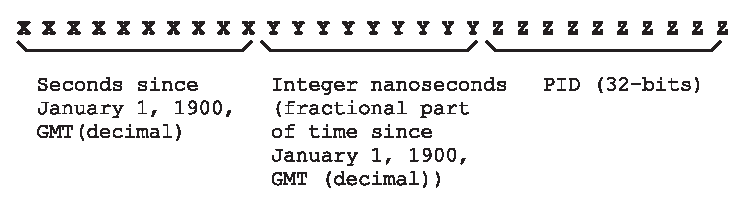
\includegraphics[width=4.6in]{c_tbg0/sguidformat01.eps}
\caption{Format of SGUID}
\label{fig:ctbg0:sdty0:ssgu0:00}
\end{figure}

Figure \ref{fig:ctbg0:sdty0:ssgu0:00} illustrates the format of
an SGUID.  An SGUID consists of 29 characters, with the following
components.

\begin{itemize}
\item \textbf{Integer seconds since the January 1, 1900 GMT (10 characters):}
      These 10 characters are an integer, zero-padded on the left as
      necessary, that represent the integer seconds since January 1, 1900
      GMT.\footnote{Note that 10 digits comfortably solves the Unix
      2037 A.D. issue, as this will guarantee SGUIDs 
      beyond 2200 A.D.}
\item \textbf{Nanoseconds associated with the integer seconds (9 characters):}
      These 9 characters are an integer, zero-padded on the left as
      necessary, that represent the nanoseconds associated with the
      integer seconds since January 1, 1900,
      GMT.\footnote{As of this writing, Linux provides time to a resolution
      of microseconds.  It is anticipated that a resolution of nanoseconds will
      accommodate any hardware speed advances in the foreseeable future, as typical
      hardware gate propagation delays are on the order of several nanoseconds.}  
\item \textbf{PID (10 characters):}
      These 10 characters are an integer, zero-padded on the left as
      necessary, that represent Unix PID expressed 
      as a decimal number.\footnote{As of this writing, PIDs are 16 bits only.
      However, it seems inevitable that PIDs will be expanded to 24 or 32 bits in the 
      future.}  
\end{itemize}

Note that SGUIDs as described have a very important property in addition to
guaranteed uniqueness---the lexical
string sort order corresponds to the time sort order.

Two sample applications of SGUIDs are:

\begin{itemize}
\item The basis for a session identifier (guaranteed unique).
\item A field in a database record to detect browser editing collisions---when a record
      is modified and a new SGUID is assigned to the record, it is \emph{guaranteed}
      not to be the same as the previous SGUID, and thus detection of the editing collision
      is guaranteed.
\end{itemize}


%%%%%%%%%%%%%%%%%%%%%%%%%%%%%%%%%%%%%%%%%%%%%%%%%%%%%%%%%%%%%%%%%%%%%%%%%%%%%%%
%%%%%%%%%%%%%%%%%%%%%%%%%%%%%%%%%%%%%%%%%%%%%%%%%%%%%%%%%%%%%%%%%%%%%%%%%%%%%%%
%%%%%%%%%%%%%%%%%%%%%%%%%%%%%%%%%%%%%%%%%%%%%%%%%%%%%%%%%%%%%%%%%%%%%%%%%%%%%%%
\subsection{SID (Session Identifier)}
%Subsection tag:  sid0
\label{ctbg0:sdty0:ssid0}

A \index{session identifier}session identifier (\index{SID}SID) is a
string consisting of exactly 69 characters used to uniquely
identify a session (Figure \ref{fig:ctbg0:sdty0:ssid0:00}).

\begin{figure}
\centering
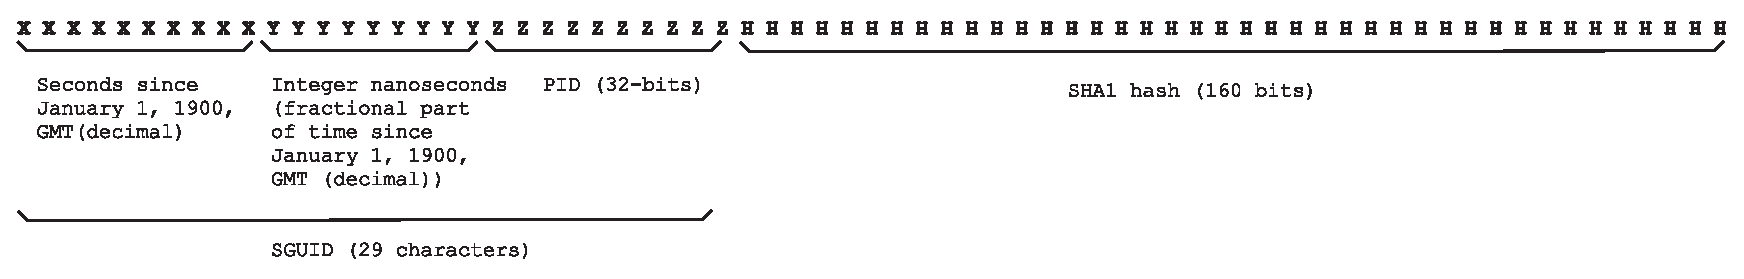
\includegraphics[width=4.6in]{c_tbg0/sidformat01.eps}
\caption{Format of SID}
\label{fig:ctbg0:sdty0:ssid0:00}
\end{figure}

The first part of the SID is a SGUID 
(\S{}\ref{ctbg0:sdty0:ssgu0}).  The second part of a SID is
the system hash function of the SGUID.  The SGUID portion is guaranteed to
be unique (this is a defining property of an SGUID),
and so each SID is unique within the first 29 characters.
The SHA1 hash appended to the SGUID is designed to eliminate an attacker's
ability to construct a valid SID.  It may be possible to guess an SGUID based
on server characteristics; but it should not be possible to guess the corresponding
hash (this is a defining property of the system hash function).

At the time a user logs in (either as a user or a guest), the SID is created
and provided to the browser as a cookie.

The session state changes that occur as \emph{\productbasename{}-\productversion{}}
is used are all stored on the server side.  The advantages of this approach
are:

\begin{itemize}
\item Only one cookie of a very short length is stored in the client's browser.
      This approach meets the RFC 2109 constraints and is also suitable
      for mobile devices.
\item An attacker's ability to gather information about the internal workings
      of \emph{\productbasename{}-\productversion{}} by
      observing cookie reassignments is severely limited
      (nothing except the SID is exposed, and exposed only once per session).
\item An attacker's ability to tamper with cookies is eliminated (only one
      cookie is provided, and it is tamper-proof).       
\end{itemize}


%%%%%%%%%%%%%%%%%%%%%%%%%%%%%%%%%%%%%%%%%%%%%%%%%%%%%%%%%%%%%%%%%%%%%%%%%%%%%%%
%%%%%%%%%%%%%%%%%%%%%%%%%%%%%%%%%%%%%%%%%%%%%%%%%%%%%%%%%%%%%%%%%%%%%%%%%%%%%%%
%%%%%%%%%%%%%%%%%%%%%%%%%%%%%%%%%%%%%%%%%%%%%%%%%%%%%%%%%%%%%%%%%%%%%%%%%%%%%%%
\section{Database Design Decisions and Discussion}
%Section tag:  ddd0
\label{ctbg0:sddd0}


%%%%%%%%%%%%%%%%%%%%%%%%%%%%%%%%%%%%%%%%%%%%%%%%%%%%%%%%%%%%%%%%%%%%%%%%%%%%%%%
%%%%%%%%%%%%%%%%%%%%%%%%%%%%%%%%%%%%%%%%%%%%%%%%%%%%%%%%%%%%%%%%%%%%%%%%%%%%%%%
%%%%%%%%%%%%%%%%%%%%%%%%%%%%%%%%%%%%%%%%%%%%%%%%%%%%%%%%%%%%%%%%%%%%%%%%%%%%%%%
\subsection{Global Scope Naming Conventions}
%Subsection tag:  gsn0
\label{ctbg0:sddd0:sgsn0}

In certain of the database tables and in certain other
contexts, a global naming convention is used rather than
further indexing information by application and page.  (For
example, the \emph{upns} and \emph{stns} tables in 
\S{}\ref{ctbg0:sddd0:scfn0}, Figure
\ref{fig:ctbg0:sddd0:scfn0:spga0:00}, p. 
\pageref{fig:ctbg0:sddd0:scfn0:spga0:00}.)

The conventions are quite loose, and simply consist of assigning names
that suggest, in order, the application, then the page, then the 
variable within the page.
If this convention is followed, applications and pages can easily
query for all the database records that affect them by using the
SQL \emph{like} clause.\footnote{It was verified that \emph{MySQL} will
perform such a query nearly instantly even with a million records, so long
as the column involved in the query is indexed and so long as the wildcard
part of the name is at the end.}

For example, a \emph{MySQL} query of the form\\\\
\texttt{SELECT * FROM tablename\\WHERE columnname LIKE 'APP\_\%' ORDER BY columnname;}\\\\
will very efficiently extract all records whose value in a column
begins with ``APP\_'', so long as the column is indexed.

Using these naming conventions, it is also possible to simulate arrays.  For
example, a variable named\\\\
\texttt{APP\_EMPCOST\_PG\_RECORDDISPLAY\_EMP\_HRS\_000029\_000042}\\\\
might be used to represent row 29 and column 42 of the underlying variable.


%%%%%%%%%%%%%%%%%%%%%%%%%%%%%%%%%%%%%%%%%%%%%%%%%%%%%%%%%%%%%%%%%%%%%%%%%%%%%%%
%%%%%%%%%%%%%%%%%%%%%%%%%%%%%%%%%%%%%%%%%%%%%%%%%%%%%%%%%%%%%%%%%%%%%%%%%%%%%%%
%%%%%%%%%%%%%%%%%%%%%%%%%%%%%%%%%%%%%%%%%%%%%%%%%%%%%%%%%%%%%%%%%%%%%%%%%%%%%%%
\subsection{\emph{MySQL} Database Locking}
%Subsection tag:  mdl0
\label{ctbg0:sddd0:smdl0}

The design of \emph{\productbasename{}-\productversion{}} includes
many tables and complex relations.  In order to ensure database
consistency, it is necessary to ensure atomicity of operations.

The approach taken to serialize database access is:

\begin{itemize}
\item Serialization is accomplished via the SQL \emph{LOCK TABLES}
      and \emph{UNLOCK TABLES} statements.

      \begin{itemize}
      \item At the start of the critical section, \emph{all} tables existing
            in the database are locked via a single \emph{LOCK TABLES}
            statement.\footnote{It was determined via newsgroup posts
            that the practical limit on the number of tables that can 
            be locked in a single SQL statement is much higher---probably
            thousands of tables---than will be encountered in practice in
            this product.  As a fallback position if locking all tables
            proves impossible, the \emph{GET\_LOCK()} 
            function and its companion function can be used.  \emph{GET\_LOCK()}
            isn't the first choice because the name is server-global rather
            than database global, and malicious code (in another database
            application) could cause denial of service.  Additionally, it has
            been verified that this method handles all the important scenarios
            such as ordinary contention, dying processes, a process that 
            terminates without releasing the lock, etc.}
      \item At the end of the critical section, a single \emph{UNLOCK TABLES}
            statement is executed.
      \end{itemize}
\item Maintenance scripts that run hot will be written to lock and unlock so that
      if there is collision with a web page, the web page will be delayed for only
      a small amount of time.
\item A recursive locking protocol is employed in the software to simplify the case
      of a critical section occurring within a critical section.  (This ensures
      in an orderly way
      that large-scope critical sections are not compromised by small-scope critical
      sections.)
\end{itemize}


%%%%%%%%%%%%%%%%%%%%%%%%%%%%%%%%%%%%%%%%%%%%%%%%%%%%%%%%%%%%%%%%%%%%%%%%%%%%%%%
%%%%%%%%%%%%%%%%%%%%%%%%%%%%%%%%%%%%%%%%%%%%%%%%%%%%%%%%%%%%%%%%%%%%%%%%%%%%%%%
%%%%%%%%%%%%%%%%%%%%%%%%%%%%%%%%%%%%%%%%%%%%%%%%%%%%%%%%%%%%%%%%%%%%%%%%%%%%%%%
\subsection{File Repository Organization}
%Subsection tag:  fro0
\label{ctbg0:sddd0:sfro0}

The \emph{\productbasename{}} software needs to maintain user-uploaded
files in conjunction with a 
database.  All such files are aggregated into one structure
called the \emph{file repository}.\index{file repository}

In the type of file repository described here, each file in the repository
has a corresponding database record containing a unique integer index.  These indices
are assigned automatically by \emph{MySQL} and are assigned sequentially
as files are added (i.e. ``1'', ``2'', ``3'', etc.).

Although
\emph{MySQL} has the capability to store files directly as part of
the database, the files are stored as distinct files directly
under the operating system for the following
reasons:

\begin{itemize}
\item The upper limit for the size of the individual and collective
      files stored directly in 
      \emph{MySQL} is not known or trusted.  (The behavior of 
      the *nix filesystem, on the other hand, is well-understood
      and trusted.)
\item The ability to split the file repository across multiple
      volumes (for disk capacity reasons) via symlinks must
      be preserved.
\item In the event of \emph{MySQL} database corruption, the files must still
      be easily recoverable.  This constraint would not be met if the
      files were stored directly in \emph{MySQL}.
\item If incremental backups are used, it is known that \emph{MySQL} tends
      to cause an entire table of files to be backed up (this can be tens
      or hundreds of megabytes or more), whereas an approach relying on discrete
      files will cause only the new or modified files to be incrementally
      backed up.
\end{itemize}

The following constraints and design goals for the file repository exist:

\begin{itemize}
\item The differential growth of disk consumption due to overhead (such as
      directory creation) as files are added
      should not be excessive under the assumption that indices grow linearly. 
\item It is known that *nix systems begin to experience performance issues
      when directories contain more than about 200 files or subdirectories (due to
      the linear search).  Any solution should not place more than about 200 files
      or subdirectories in a directory.
\item The solution should facilitate symlinking to split the file
      repository across multiple volumes.
\item The solution must accommodate logical indices as large as $2^{64}-1$.\footnote{This design
      goal applies because \emph{MySQL} allows 64-bit integers to be used as the primary
      key for database tables.}
\item The solution must allow files to be aged out or deleted
      randomly with respect to the integer indices (to comply with records retention
      policies, because they are removed from the repository, or for other reasons).
\end{itemize}

In order to accommodate the constraints, files are stored in a directory structure
based on prime moduli of the database integer index $n$.  
The lowest level of the directory structure contains a single
file per directory, with the lowest-level directory named being the 
decimal representation of the
integer index $n$.

The definining equations for the directory path components are supplied below.

\begin{eqnarray}
\label{eq:ctbg0:sddd0:sfro0:00}   d    & = & 160                               \\
\label{eq:ctbg0:sddd0:sfro0:01} c_0    & = & \lfloor n / d \rfloor \bmod 7   \\
\label{eq:ctbg0:sddd0:sfro0:02} c_1    & = & \lfloor n / d \rfloor \bmod 11  \\ 
\label{eq:ctbg0:sddd0:sfro0:03} c_2    & = & \lfloor n / d \rfloor \bmod 13  \\
\label{eq:ctbg0:sddd0:sfro0:04} c_3    & = & \lfloor n / d \rfloor \bmod 89  \\
\label{eq:ctbg0:sddd0:sfro0:05} c_4    & = & \lfloor n / d \rfloor \bmod 97  \\
\label{eq:ctbg0:sddd0:sfro0:06} c_5    & = & \lfloor n / d \rfloor \bmod 101 \\
\label{eq:ctbg0:sddd0:sfro0:07} c_6    & = & \lfloor n / d \rfloor \bmod 103 \\
\label{eq:ctbg0:sddd0:sfro0:08} c_7    & = & \lfloor n / d \rfloor \bmod 107 \\
\label{eq:ctbg0:sddd0:sfro0:09} c_8    & = & \lfloor n / d \rfloor \bmod 109 \\
\label{eq:ctbg0:sddd0:sfro0:10} c_9    & = & \lfloor n / d \rfloor \bmod 113 
\end{eqnarray}

With reference to (\ref{eq:ctbg0:sddd0:sfro0:01})
through (\ref{eq:ctbg0:sddd0:sfro0:10}), the relative path within a file repository
to the directory containing a file with database index $n$ is\\
``$c_0$/$c_1$/$c_2$/$c_3$/$c_4$/$c_5$/$c_6$/$c_7$/$c_8$/$c_9$/$n$''\@.
Each path component $c_i$ and $n$ is the traditional human-friendly variable-length
representation:
for example, ``3'', ``25'', ```111', or ``36237456726''.  

Note that the storage scheme proposed will handle indices 
as large as $2^{64}-1$, i.e.

\begin{equation}
\label{eq:ctbg0:sddd0:sfro0:20}
d \times c_0 \times c_1 \times c_2 \times c_3 \times c_4
\times c_5 \times c_6 \times c_7 \times c_8 \times c_9 > 2^{64} - 1 .
\end{equation}

Note also that the first three
components ($c_0$, $c_1$, and $c_2$) are small and chosen for 
convenient symlinking, whereas the last seven components ($c_3$ through $c_9$)
are chosen to increase the product rapidly while staying clear of the 
*nix performance limit of approximately 200 entries per directory.

Two properties of the storage scheme proposed by (\ref{eq:ctbg0:sddd0:sfro0:01})
through (\ref{eq:ctbg0:sddd0:sfro0:10}) may require further explanation.

\begin{itemize}
\item The differential cost of storing a file in the repository is
      approximately the file size (with operating system overhead)
      plus approximately 1.0625 directories.  This comes about because
      every file requires its own directory, and because
      every 160 files, 10 directories must be created.
\item If the index $n$ increases linearly, the number of files stored in
      each directory (especially at the top levels) will be approximately
      equal.  (The reason for this is the coprimality of the divisors
      used.  The necessary proof comes from number theory, and isn't 
      included here.)  This means that symlinking at the top levels will be
      effective in evenly dividing storage requirements.
\end{itemize}


%%%%%%%%%%%%%%%%%%%%%%%%%%%%%%%%%%%%%%%%%%%%%%%%%%%%%%%%%%%%%%%%%%%%%%%%%%%%%%%
%%%%%%%%%%%%%%%%%%%%%%%%%%%%%%%%%%%%%%%%%%%%%%%%%%%%%%%%%%%%%%%%%%%%%%%%%%%%%%%
%%%%%%%%%%%%%%%%%%%%%%%%%%%%%%%%%%%%%%%%%%%%%%%%%%%%%%%%%%%%%%%%%%%%%%%%%%%%%%%
\subsection{Database Design to Support Core Functionality}
%Subsection tag:  cfn0
\label{ctbg0:sddd0:scfn0}

The core functionality as described in Chapter \ref{ccfn0} consists of:

\begin{itemize}
\item Site navigation (\S{}\ref{ccfn0:ssng0}).
\item Authentication and login (\S{}\ref{ccfn0:salg0}).
\item Permission groups and attributes (\S{}\ref{ccfn0:sgra0}).
\item Notification (\S{}\ref{ccfn0:snot0}).
\item Action list (\S{}\ref{ccfn0:sacl0}).
\item Logging (\S{}\ref{ccfn0:slog0}).
\end{itemize}

Figure \ref{fig:ctbg0:sddd0:scfn0:spga0:00} provides an overview of the
tables involved in implementing the core functionality.  In the figure,
for efficiency, note that three of the most frequently
used read-only tables (\emph{applications}, \emph{pages},
and \emph{navlines}) are implemented as lookup tables in 
\emph{PHP} rather than
as \emph{MySQL} tables.\footnote{Presumably, the \emph{PHP}
interpreter parsing these tables is far more efficient than executing
an SQL query and processing the results.}

\begin{figure}
\centering
\includegraphics[width=4.6in]{c_tbg0/dbdesign01.eps}
\caption{User, Permission Group, Application, and Page Database Design}
\label{fig:ctbg0:sddd0:scfn0:spga0:00}
\end{figure}


%%%%%%%%%%%%%%%%%%%%%%%%%%%%%%%%%%%%%%%%%%%%%%%%%%%%%%%%%%%%%%%%%%%%%%%%%%%%%%%
%%%%%%%%%%%%%%%%%%%%%%%%%%%%%%%%%%%%%%%%%%%%%%%%%%%%%%%%%%%%%%%%%%%%%%%%%%%%%%%
%%%%%%%%%%%%%%%%%%%%%%%%%%%%%%%%%%%%%%%%%%%%%%%%%%%%%%%%%%%%%%%%%%%%%%%%%%%%%%%
\subsubsection{Users and Tokens}
%Subsubsection tag:  utk0
\label{ctbg0:sddd0:scfn0:sutk0}

The database design includes a table of users (the \emph{users} table
in Figure \ref{fig:ctbg0:sddd0:scfn0:spga0:00}).  Each user who can log
in to the system has one record in this table.  As mentioned
in \S{}????, each user always logs in using a userid that 
represents the user---there
are no userids used solely for administration.

The \emph{users} table 
(Figure \ref{fig:ctbg0:sddd0:scfn0:spga0:00}) is related 1:1 with the
\emph{tokens} table.
Each user is optionally assigned a cryptographic token to use in
authenticating.  Token assignment is on a per-user
basis, so that \emph{\productbasename{}-\productversion{}} will support:

\begin{itemize}
\item No users authenticating using cryptographic tokens.
\item Some users authenticating with cryptographic tokens, and some authenticating
      without cryptographic tokens.
\item All users authenticating with cryptographic tokens.
\end{itemize}


%%%%%%%%%%%%%%%%%%%%%%%%%%%%%%%%%%%%%%%%%%%%%%%%%%%%%%%%%%%%%%%%%%%%%%%%%%%%%%%
%%%%%%%%%%%%%%%%%%%%%%%%%%%%%%%%%%%%%%%%%%%%%%%%%%%%%%%%%%%%%%%%%%%%%%%%%%%%%%%
%%%%%%%%%%%%%%%%%%%%%%%%%%%%%%%%%%%%%%%%%%%%%%%%%%%%%%%%%%%%%%%%%%%%%%%%%%%%%%%
\subsubsection{User Permission Attributes}
%Subsubsection tag:  pga0
\label{ctbg0:sddd0:scfn0:spga0}

Figure \ref{fig:ctbg0:sddd0:scfn0:spga0:00} shows that the \emph{users} and 
\emph{upermattrs} tables are related by the \emph{userupermattrs} table, providing 
an $\infty{}:\infty{}$ mapping.

Each record in the \emph{userupermattrs} table also carries with it an
optional string.  Such as string is interpreted as a user-specific value of the
related record in the \emph{upermattrs} table.  As a 
contrived example, one user may have
a value of MAX\_LOGINS of 2, and another user may have a value of 5.

If the optional string in the \emph{userupermattrs} table is the empty string,
then the $\infty{}:\infty{}$ relation effectively specifies a named set
of users.  Such named sets are typically used to control user permissions
in a fine-grained way---a given group may contain the users who can add
products to the \emph{products} table, for example.


%%%%%%%%%%%%%%%%%%%%%%%%%%%%%%%%%%%%%%%%%%%%%%%%%%%%%%%%%%%%%%%%%%%%%%%%%%%%%%%
%%%%%%%%%%%%%%%%%%%%%%%%%%%%%%%%%%%%%%%%%%%%%%%%%%%%%%%%%%%%%%%%%%%%%%%%%%%%%%%
%%%%%%%%%%%%%%%%%%%%%%%%%%%%%%%%%%%%%%%%%%%%%%%%%%%%%%%%%%%%%%%%%%%%%%%%%%%%%%%
\subsubsection{User Persistent Named State}
%Subsubsection tag:  upn0
\label{ctbg0:sddd0:scfn0:supn0}

User permission attributes do not change as the result of ordinary usage of
the \emph{\productbasename{}-\productversion{}} system.  Although 
user permission attributes can be modified, this is an administrative action
and does not happen often.

For state bound to a user which may change often, the 
\emph{upns} table (Figure \ref{fig:ctbg0:sddd0:scfn0:spga0:00}) is
provided.  This state is very similar in spirit to what may be contained
in the \emph{Windows} registry.

Each record in the \emph{upns} table consists of a name and a value.

For each user, the names in the \emph{upns} table must be unique (no
duplicates are allowed).

A naming convention is used so that each entry in the \emph{upns} table
is bound to a specific application and page.  The \emph{upns} table is indexed
by name for fast retrieval.


%%%%%%%%%%%%%%%%%%%%%%%%%%%%%%%%%%%%%%%%%%%%%%%%%%%%%%%%%%%%%%%%%%%%%%%%%%%%%%%
%%%%%%%%%%%%%%%%%%%%%%%%%%%%%%%%%%%%%%%%%%%%%%%%%%%%%%%%%%%%%%%%%%%%%%%%%%%%%%%
%%%%%%%%%%%%%%%%%%%%%%%%%%%%%%%%%%%%%%%%%%%%%%%%%%%%%%%%%%%%%%%%%%%%%%%%%%%%%%%
\subsubsection{Sessions}
%Subsubsection tag:  ses0
\label{ctbg0:sddd0:scfn0:sses0}

A \emph{session} is the relationship between the server and a client during
a single login (whether as a named user or a guest).

Sessions are stored in the \emph{sessions} table 
(Figure \ref{fig:ctbg0:sddd0:scfn0:spga0:00}).  Each record in the 
\emph{sessions} table contains the session identifier, information about the
user, information about the time of the last actions associated with the
session, etc.


%%%%%%%%%%%%%%%%%%%%%%%%%%%%%%%%%%%%%%%%%%%%%%%%%%%%%%%%%%%%%%%%%%%%%%%%%%%%%%%
%%%%%%%%%%%%%%%%%%%%%%%%%%%%%%%%%%%%%%%%%%%%%%%%%%%%%%%%%%%%%%%%%%%%%%%%%%%%%%%
%%%%%%%%%%%%%%%%%%%%%%%%%%%%%%%%%%%%%%%%%%%%%%%%%%%%%%%%%%%%%%%%%%%%%%%%%%%%%%%
\subsubsection{Session Temporary Named State}
%Subsubsection tag:  stn0
\label{ctbg0:sddd0:scfn0:sstn0}

State that should be stored associated with a session rather than a user
(i.e. that should be deleted when a session ends) is stored in the
\emph{stns} table (Figure \ref{fig:ctbg0:sddd0:scfn0:spga0:00}).

Each entry in the \emph{stns} table consists of a name and a value.
Within each session, each name in the \emph{stns} table must be unique.

A naming convention is used so that each entry in the \emph{stns} table
is bound to a specific application and page.  The \emph{stns} table is indexed
by name for fast retrieval.


%%%%%%%%%%%%%%%%%%%%%%%%%%%%%%%%%%%%%%%%%%%%%%%%%%%%%%%%%%%%%%%%%%%%%%%%%%%%%%%
%%%%%%%%%%%%%%%%%%%%%%%%%%%%%%%%%%%%%%%%%%%%%%%%%%%%%%%%%%%%%%%%%%%%%%%%%%%%%%%
%%%%%%%%%%%%%%%%%%%%%%%%%%%%%%%%%%%%%%%%%%%%%%%%%%%%%%%%%%%%%%%%%%%%%%%%%%%%%%%
\subsubsection{Chain of Command}
%Subsubsection tag:  coc0
\label{ctbg0:sddd0:scfn0:scoc0}

In some contexts, \emph{\productbasename{}-\productversion{}} components
need to make decisions based on reporting relationships between
employees.  For example, some information about an employee should only
be viewable or editable by those above the employee in the chain of command.

The database contains an \emph{enterprises} table
(Figure \ref{fig:ctbg0:sddd0:scfn0:spga0:00}) and an
\emph{usersenterprises} table that provide a 
$\infty{}:\infty{}$ mapping between \emph{users}
and \emph{enterprises}.  A given user may belong to more than one 
enterprise and may exist in reporting relationships in more than
one enterprise.

The database also contains a \emph{cocrels} table
(Figure \ref{fig:ctbg0:sddd0:scfn0:spga0:00}) that can capture
reporting relationships between employees for each enterprise.  
Both normal reporting relationships
and matrix reporting relationships can be captured.


%%%%%%%%%%%%%%%%%%%%%%%%%%%%%%%%%%%%%%%%%%%%%%%%%%%%%%%%%%%%%%%%%%%%%%%%%%%%%%%
%%%%%%%%%%%%%%%%%%%%%%%%%%%%%%%%%%%%%%%%%%%%%%%%%%%%%%%%%%%%%%%%%%%%%%%%%%%%%%%
%%%%%%%%%%%%%%%%%%%%%%%%%%%%%%%%%%%%%%%%%%%%%%%%%%%%%%%%%%%%%%%%%%%%%%%%%%%%%%%
\subsubsection{Login Attempts}
%Subsubsection tag:  lat0
\label{ctbg0:sddd0:scfn0:slat0}

The database contains a \emph{loginattempts} table
(Figure \ref{fig:ctbg0:sddd0:scfn0:spga0:00}).
The \emph{loginattempts} records unsuccessful login attempts that meet criteria
in order to implement security policies that involve the maximum number of
certain types of login attempts in a period of time.\footnote{In principle,
the \emph{logentries} table also contains enough information to implement
security policies, but the design is more versatile if a separate table
is used for this purpose.}


%%%%%%%%%%%%%%%%%%%%%%%%%%%%%%%%%%%%%%%%%%%%%%%%%%%%%%%%%%%%%%%%%%%%%%%%%%%%%%%
%%%%%%%%%%%%%%%%%%%%%%%%%%%%%%%%%%%%%%%%%%%%%%%%%%%%%%%%%%%%%%%%%%%%%%%%%%%%%%%
%%%%%%%%%%%%%%%%%%%%%%%%%%%%%%%%%%%%%%%%%%%%%%%%%%%%%%%%%%%%%%%%%%%%%%%%%%%%%%%
\subsubsection{User Templates}
%Subsubsection tag:  utp0
\label{ctbg0:sddd0:scfn0:sutp0}

In a mature deployment of \emph{\productbasename{}-\productversion{}},
a typical user may have dozens of associated permission attributes.
Creating a new user would be quite tedious if a complex set of permission 
attributes need to be created at the same time.

To make this process easier, user templates are provided via the 
\emph{utemplates} and \emph{utemplatespermgroups} tables depicted in
Figure \ref{fig:ctbg0:sddd0:scfn0:spga0:00}.  A user template gives
a one-click way to create a user with a complex set of permission attributes.

A user template contains the same type of $\infty{}:\infty{}$
relation to the \emph{permattrs} table as a user.  Creating a new user
from a user template is a relatively straightforward process of copying.

In general, a user may create another user if and only if:

\begin{itemize}
\item The user has the permission attribute set to be able to create
      other users.
\item The security level integer of the created user is greater than that of
      the creating user.
\item All ranked permission attributes of the created user are inferior to those of
      the creating user.
\end{itemize}


%%%%%%%%%%%%%%%%%%%%%%%%%%%%%%%%%%%%%%%%%%%%%%%%%%%%%%%%%%%%%%%%%%%%%%%%%%%%%%%
%%%%%%%%%%%%%%%%%%%%%%%%%%%%%%%%%%%%%%%%%%%%%%%%%%%%%%%%%%%%%%%%%%%%%%%%%%%%%%%
%%%%%%%%%%%%%%%%%%%%%%%%%%%%%%%%%%%%%%%%%%%%%%%%%%%%%%%%%%%%%%%%%%%%%%%%%%%%%%%
\subsubsection{Site Navigation}
%Subsubsection tag:  snv0
\label{ctbg0:sddd0:scfn0:ssnv0}

The left navigation pane of the \emph{\productbasename{}-\productversion{}}
displays a hierarchical set of links to pages.  The left navigation page
is hierarchical in the sense that links to pages may be displayed under headings
or sub-headings.  The logic used to
display links is:

\begin{itemize}
\item Each page in the \emph{pages} table contains a set of \emph{permgroups}.
      Any user must be a member of at least one of the set of \emph{permgroups}
      in order for the link to the page to be displayed (and in order to use
      the services of the page at all).
\item A heading or sub-heading is displayed if and only if there is at least
      one page link under the heading or sub-heading that, based on 
      the required \emph{permgroups}, should be displayed.  (Headings and
      sub-headings automatically drop out when there are no page links under
      them.)
\end{itemize}

The relationship between 
\emph{applications}, \emph{pages}, and \emph{navlines} shown
in Figure \ref{fig:ctbg0:sddd0:scfn0:spga0:00} has these
elements:

\begin{itemize}
\item \emph{applications} have a $1:\infty$ relationship with the
      \emph{pages}.  Every page is a member of exactly one application.
\item The \emph{navlines} specify the headings and page links that may appear
      (depending on \emph{permgroups}) in the left navigation pane.  A given page
      may appear in more than one location in the left navigation pane (hence
      the $\infty{}:1$ relationship\footnote{With the additional caveat that
      a page is not required to appear in the left navigation pane---some pages
      can only be reached indirectly.}).
\end{itemize}

Note that the \emph{pages} and \emph{applications} tables are linked to
from other tables (these relationships are not shown due to complexity constraints
in Figure \ref{fig:ctbg0:sddd0:scfn0:spga0:00}).  For
example, the \emph{globalvars} table is linked by page and application
so that the variables relevant to a page can be extracted more economically.


%%%%%%%%%%%%%%%%%%%%%%%%%%%%%%%%%%%%%%%%%%%%%%%%%%%%%%%%%%%%%%%%%%%%%%%%%%%%%%%
%%%%%%%%%%%%%%%%%%%%%%%%%%%%%%%%%%%%%%%%%%%%%%%%%%%%%%%%%%%%%%%%%%%%%%%%%%%%%%%
%%%%%%%%%%%%%%%%%%%%%%%%%%%%%%%%%%%%%%%%%%%%%%%%%%%%%%%%%%%%%%%%%%%%%%%%%%%%%%%
\subsubsection{Products and Product Components}
%Subsubsection tag:  pcn0
\label{ctbg0:sddd0:scfn0:spcn0}

The \emph{products}, \emph{pcomponents}, \emph{psubcomponents}, 
and \emph{pversions} tables in Figure \ref{fig:ctbg0:sddd0:scfn0:spga0:00}
define the products that are produced.  Note that a version can only
be associated with a product (rather than a component or subcomponent
of a product).

The exact semantics of what constitutes a product, product component,
and product subcomponent is naturally dependent on the organization.


%%%%%%%%%%%%%%%%%%%%%%%%%%%%%%%%%%%%%%%%%%%%%%%%%%%%%%%%%%%%%%%%%%%%%%%%%%%%%%%
%%%%%%%%%%%%%%%%%%%%%%%%%%%%%%%%%%%%%%%%%%%%%%%%%%%%%%%%%%%%%%%%%%%%%%%%%%%%%%%
%%%%%%%%%%%%%%%%%%%%%%%%%%%%%%%%%%%%%%%%%%%%%%%%%%%%%%%%%%%%%%%%%%%%%%%%%%%%%%%
\subsubsection{File Repository Organization}
%Subsubsection tag:  fro0
\label{ctbg0:sddd0:scfn0:sfro0}

The information maintained about the file repository files in the
\emph{MySQL} database is maintained in the \emph{frfiles},
\emph{frfilesfrfusages}, and \emph{frfusages} tables
(Figure \ref{fig:ctbg0:sddd0:scfn0:spga0:00}).  These three
tables create a $\infty{}:\infty{}$ mapping between
the \emph{frfiles} and \emph{frfusages} tables.

The \emph{frfiles} table contains one record per file in the
file repository.  Each of these records contains all direct information
about the stored file (location, SHA1 hash value, etc.).

The \emph{frfilesfrfusages} and \emph{frfusages} tables are necessary because
there are PHP scripts that:

\begin{itemize}
\item Display information about a file in the file repository.
\item Serve the contents of a file in the file repository.
\end{itemize}

These scripts must be able to determine whether a given user is authorized to
view information about a file repository file or download the file.
The difficulty in making this determination is that the file repository is
is shared among many applications.  Without some sort of a hint, the process
of determining whether a user may view information about a repository file
or download it would be an iterative process of checking every
\emph{\productbasename{}-\productversion{}} application to determine if it
has involvement with the repository file and if the user has permissions for the
file.  The \emph{frfusages} table is a table of possible usages for a file 
repository file.  Using this table, the applications to check for file permissions
should be reduced in a typical case to one or two.

At the present time, each usage of a file repository file is simply
an integer, and so the \emph{frfusages} is superfluous (the integer could
simply be stored directly in the \emph{frfilesfrusages} table).  However,
the more complex schema is used in case future expansion or enhancement 
occurs.


%%%%%%%%%%%%%%%%%%%%%%%%%%%%%%%%%%%%%%%%%%%%%%%%%%%%%%%%%%%%%%%%%%%%%%%%%%%%%%%
%%%%%%%%%%%%%%%%%%%%%%%%%%%%%%%%%%%%%%%%%%%%%%%%%%%%%%%%%%%%%%%%%%%%%%%%%%%%%%%
%%%%%%%%%%%%%%%%%%%%%%%%%%%%%%%%%%%%%%%%%%%%%%%%%%%%%%%%%%%%%%%%%%%%%%%%%%%%%%%
\subsubsection{Global Variables}
%Subsubsection tag:  gvr0
\label{ctbg0:sddd0:scfn0:sgvr0}

The database includes a table of global variables 
(the \emph{globalvars} table in Figure \ref{fig:ctbg0:sddd0:scfn0:spga0:00},
p. \pageref{fig:ctbg0:sddd0:scfn0:spga0:00}).

Global variables have these uses:

\begin{itemize}
\item Influencing the behavior of applications (global variables often override
      default behavior---similar to the typical behavior of \emph{Unix} environment
      variables).  For example, the web interface to the database can be taken
      offline by setting a global variable.
\item Mutual exclusion:  for example, a global variable is used to ensure that two instances
      of the maintenance script don't run concurrently.
\item Application persistent state:  state that is not bound to a user or a session
      (discussed later) can be stored in global variables (similar to the behavior of
      the \emph{Windows} registry).
\end{itemize}

Global variables have these essential characteristics:

\begin{itemize}
\item The name of a global variable must be unique (duplicate names in the 
      \emph{globalvars} table are not allowed).  In order to facilitate and 
      guarantee uniqueness, a naming convention
      (\S{}\ref{ctbg0:sddd0:sgsn0}, p. \pageref{ctbg0:sddd0:sgsn0}) is used that
      names the global variables by application then page.
\item The \emph{globalvars} table is indexed by variable name.
\end{itemize}


%%%%%%%%%%%%%%%%%%%%%%%%%%%%%%%%%%%%%%%%%%%%%%%%%%%%%%%%%%%%%%%%%%%%%%%%%%%%%%%
%%%%%%%%%%%%%%%%%%%%%%%%%%%%%%%%%%%%%%%%%%%%%%%%%%%%%%%%%%%%%%%%%%%%%%%%%%%%%%%
%%%%%%%%%%%%%%%%%%%%%%%%%%%%%%%%%%%%%%%%%%%%%%%%%%%%%%%%%%%%%%%%%%%%%%%%%%%%%%%
\subsubsection{Logging}
%Subsubsection tag:  log0
\label{ctbg0:sddd0:scfn0:slog0}

\emph{\productbasename{}-\productversion{}} maintains a log in the form of
a database table (the \emph{logentries} table in Figure \ref{fig:ctbg0:sddd0:scfn0:spga0:00},
p. \pageref{fig:ctbg0:sddd0:scfn0:spga0:00}).  This database table
contains indexed columns so that the log can be viewed based on
chronological order, application, log entry type, and security threat level.


%%%%%%%%%%%%%%%%%%%%%%%%%%%%%%%%%%%%%%%%%%%%%%%%%%%%%%%%%%%%%%%%%%%%%%%%%%%%%%%
%%%%%%%%%%%%%%%%%%%%%%%%%%%%%%%%%%%%%%%%%%%%%%%%%%%%%%%%%%%%%%%%%%%%%%%%%%%%%%%
%%%%%%%%%%%%%%%%%%%%%%%%%%%%%%%%%%%%%%%%%%%%%%%%%%%%%%%%%%%%%%%%%%%%%%%%%%%%%%%
\subsubsection{Inbox}
%Subsubsection tag:  inb0
\label{ctbg0:sddd0:scfn0:sinb0}

When certain events/actions occur, one or more users should be notified.
The notices are inserted into the \emph{inbox} table 
(Figure \ref{fig:ctbg0:sddd0:scfn0:spga0:00}).

Presently, only the \emph{inbox} is implemented, and is used only for
automatic notifications from applications.  In the future, a more general messaging
system (with the ability to send/receive e-mail or the ability to send/receive
messages to other users) may be implemented.


%%%%%%%%%%%%%%%%%%%%%%%%%%%%%%%%%%%%%%%%%%%%%%%%%%%%%%%%%%%%%%%%%%%%%%%%%%%%%%%
%%%%%%%%%%%%%%%%%%%%%%%%%%%%%%%%%%%%%%%%%%%%%%%%%%%%%%%%%%%%%%%%%%%%%%%%%%%%%%%
%%%%%%%%%%%%%%%%%%%%%%%%%%%%%%%%%%%%%%%%%%%%%%%%%%%%%%%%%%%%%%%%%%%%%%%%%%%%%%%
\subsubsection{Host E-mail Preferences}
%Subsubsection tag:  hep0
\label{ctbg0:sddd0:scfn0:shep0}

Notifications are always sent to the \emph{inbox} and can be viewed by the user.
For each user, it can be configured whether notifications are also sent to
the user's e-mail address(es).

There are two concerns with injecting e-mail bound for remote hosts:

\begin{itemize}
\item Some remote hosts may filter for SPAM by limiting the number of
      e-mails that can delivered from a certain host.  With these remote hosts,
      e-mail injection must be rate-limited.
\item A software bug could result in a large number of notifications erroneously
      created.  Rate-limiting all e-mail injections for remote hosts is prudent.      
\end{itemize}

The \emph{hostemailprefs} table (Figure \ref{fig:ctbg0:sddd0:scfn0:spga0:00})
is a table of regular expressions designed to match e-mail addresses.
During the high-frequency maintenance script, the \emph{hostemailprefs}
records are scanned in a specific order in an attempt to match
the outgoing e-mail address.  The data in the first match is used to control
the generation of outgoing e-mail.

Note that generation of outgoing notification e-mail is simply a process of
sending each message in the \emph{inbox} table subject to user preferences
and rules in the \emph{hostemailprefs} table. 


%%%%%%%%%%%%%%%%%%%%%%%%%%%%%%%%%%%%%%%%%%%%%%%%%%%%%%%%%%%%%%%%%%%%%%%%%%%%%%%
%%%%%%%%%%%%%%%%%%%%%%%%%%%%%%%%%%%%%%%%%%%%%%%%%%%%%%%%%%%%%%%%%%%%%%%%%%%%%%%
%%%%%%%%%%%%%%%%%%%%%%%%%%%%%%%%%%%%%%%%%%%%%%%%%%%%%%%%%%%%%%%%%%%%%%%%%%%%%%%
\section{Product Design Decisions and Discussion}
%Section tag:  ddc0
\label{ctbg0:sddc0}


%%%%%%%%%%%%%%%%%%%%%%%%%%%%%%%%%%%%%%%%%%%%%%%%%%%%%%%%%%%%%%%%%%%%%%%%%%%%%%%
%%%%%%%%%%%%%%%%%%%%%%%%%%%%%%%%%%%%%%%%%%%%%%%%%%%%%%%%%%%%%%%%%%%%%%%%%%%%%%%
%%%%%%%%%%%%%%%%%%%%%%%%%%%%%%%%%%%%%%%%%%%%%%%%%%%%%%%%%%%%%%%%%%%%%%%%%%%%%%%
\subsection{Two-Factor Authentication}\index{two-factor authentication}
%Subection tag:  tfa0
\label{ctbg0:sddc0:stfa0}

\emph{Two-factor authentication}\index{two-factor authentication} is the practice of 
authenticating users based on both something the user \emph{knows} (typically a password)
and something the user \emph{has} (typically a cryptographic token).

It is anticipated that \emph{\productbasename{}} will be used from airport
kiosks and other locations where password capture is a very tangible possibility.

The best known countermeasure against password capture and password guessing is
one-time passwords\index{one-time password} (OTPs) generated by a
cryptographic token.  

OTPs generated by a cryptographic token are effective against password capture because
each one-time password generated can be used only once and is useless in the future.
OTP capture is not helpful to an attacker.

OTPs generated by a cryptographic token are effective against password guessing
because the OTPs generated have an approximately uniform
distribution across the space of all
OTPs that can be generated.  This is unlike passwords generated by humans,
which tend to involve language words and may facilitate guessing.


%%%%%%%%%%%%%%%%%%%%%%%%%%%%%%%%%%%%%%%%%%%%%%%%%%%%%%%%%%%%%%%%%%%%%%%%%%%%%%%
%%%%%%%%%%%%%%%%%%%%%%%%%%%%%%%%%%%%%%%%%%%%%%%%%%%%%%%%%%%%%%%%%%%%%%%%%%%%%%%
%%%%%%%%%%%%%%%%%%%%%%%%%%%%%%%%%%%%%%%%%%%%%%%%%%%%%%%%%%%%%%%%%%%%%%%%%%%%%%%
\subsubsection{Overview of the Solution}
%Subsubsection tag:  ovs0
\label{ctbg0:sddc0:stfa0:sovs0}

%Note to self:  .JPG was converted to .EPS on *nix box using
%"convert cckt1_01.jpg cckt1_01.eps", with no additonal options
%or qualifiers.  .EPS ended up to be quite large.
%
\begin{figure}
\centering
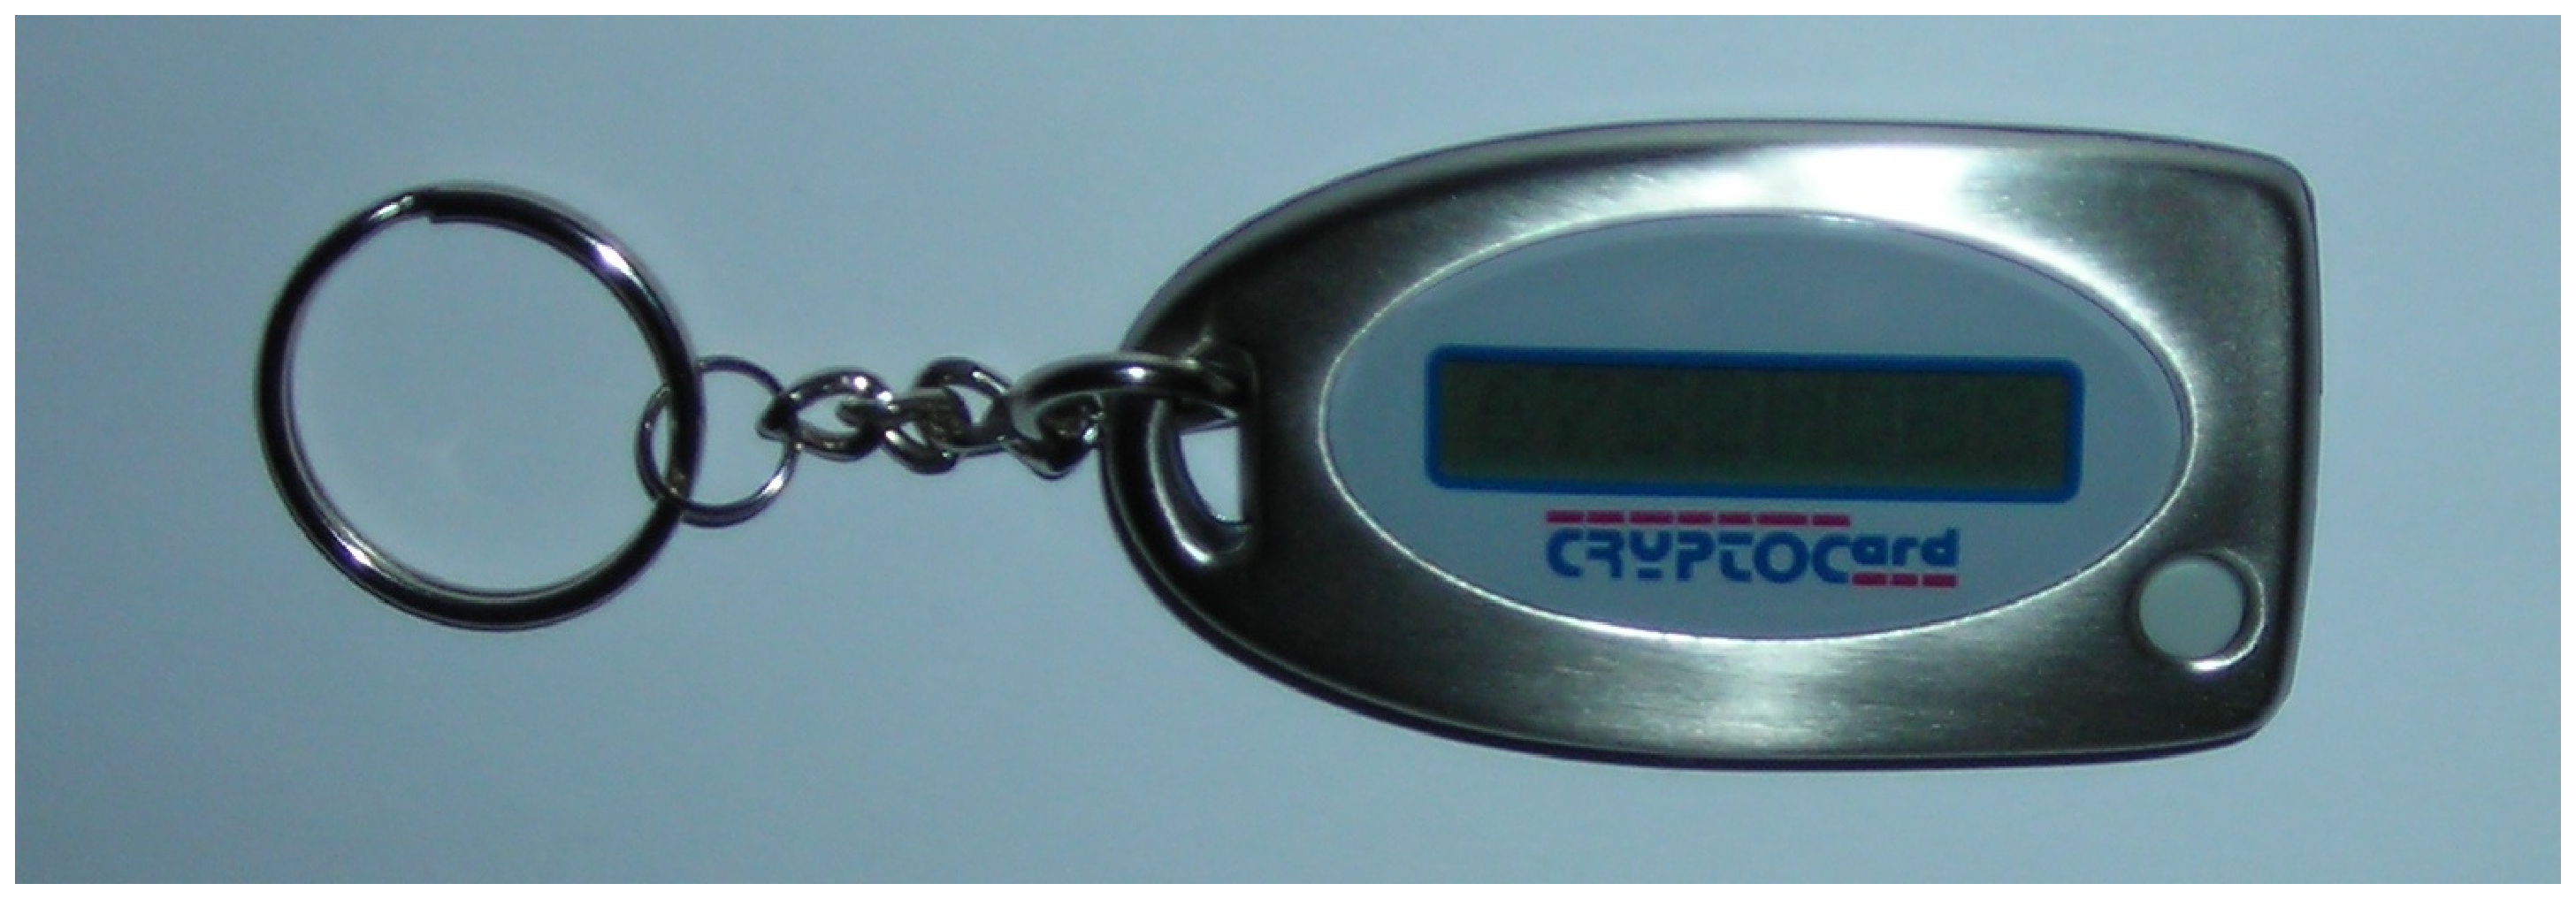
\includegraphics[width=4.6in]{c_tbg0/cckt1_01.eps}
\caption{CryptoCard KT-1 Keychain Token}
\label{fig:ctbg0:sddc0:stfa0:sovs0:00}
\end{figure}

The model of token supported by \emph{\productbasename{}}
is the CryptoCard\index{CryptoCard Corporation} 
KT-1 keychain token\index{KT-1 keychain cryptographic token} 
(Fig. \ref{fig:ctbg0:sddc0:stfa0:sovs0:00}).


On a per-user basis, logins to \emph{\productbasename{}} may be either with:

\begin{itemize}
\item Userid and password.
\item Userid, password, and OTP. 
\end{itemize}

The cryptographic basis of the CryptoCard KT-1 token and similar products
is that:

\begin{itemize}
\item The token is programmed with a key that cannot be extracted\footnote{The
      ability to extract the key from the token is equivalent to being able
      to predict all future OTPs that will be generated by the token, and hence
      would render the token useless as a security device.}, and this key is known
      to the \emph{\productbasename{}} software.
\item Mathematically, there is no way to reverse-engineer the key by observing
      OTPs generated by the token; hence there is no way to predict future
      OTPs generated by the token based on observing past OTPs.
\end{itemize}

\emph{\productbasename{}} utilizes the CryptoCard KT-1 token configured
so that each of the 8 displayed OTP characters can be one of 32 different
possibilities.\footnote{The KT-1 token can also be configured so that 
each of the 8 OTP characters can be one of 64 possibilities, leading to
$64^8 = 2.8 \times 10^{14}$ OTPs.  The base-32
OTPs were chosen because they are case-insensitive and lead to fewer user 
data entry errors.}  
The number of possible OTPs is thus $32^8 = 1.1 \times 10^{12}$.
The large number of OTPs makes a brute-force attack unattractive---even with 10 guesses
per second, the expected time to guess an OTP would be 1,700 years.

The CryptoCard KT-1 keychain token is an event-driven device---it generates
sequential OTPs according to a mathematical sequence, with one OTP generated
at each activation of the token.  The \productbasename{} software, because
it has access to the token key, is able to predict the OTPs that should be
generated by the token.  The \productbasename{} software also allows approximately
three\footnote{Configurable:  three is the default value.}
of the predicted sequential OTPs to be used, in case the KT-1 token was activated
and the OTP never used.\footnote{This might happen, for example, if the token button
is accidentally pressed by objects in the user's pockets, or if children are
allowed to play with the token.}

It can occur, however, that the KT-1 token falls out of synchronization with
the \productbasename{} software.  In this case, the token allows a resynchronization
procedure where the user enters a resynchronization string (8 digits,
allowing for $10^8$ different values).  When the token is supplied
with a resynchronization string, it resets its internal state and provides
an OTP.  This procedure allows the token and the \productbasename{} software
to be brought back into synchronization.

Note to self:  in conversation with Bill LaHam in late October 2009, Bill indicated
that the traditional approach with tokens is to have an inner window and an outer
window.  A typical inner window might be of size 3, and a typical outer window might
be of size 1000.

\begin{itemize}
\item If the token value falls within the inner window, it is authenticated without
      any other verification steps.
\item If the token value is not within the inner window but is within the outer
      window, two (additional?) consecutive values are required for authentication.
\item If the token value is not within the inner window and not within the
      outer window, some sort of resynchronization is required.
\end{itemize}

The size of the inner window is a major security risk (it raises the probability
of a successful guess), so it should be small.  The outer window is not a security
concern at all.

Need to incorporate the information from Bill into this document and the
strategy in this documennt.


%%%%%%%%%%%%%%%%%%%%%%%%%%%%%%%%%%%%%%%%%%%%%%%%%%%%%%%%%%%%%%%%%%%%%%%%%%%%%%%
%%%%%%%%%%%%%%%%%%%%%%%%%%%%%%%%%%%%%%%%%%%%%%%%%%%%%%%%%%%%%%%%%%%%%%%%%%%%%%%
%%%%%%%%%%%%%%%%%%%%%%%%%%%%%%%%%%%%%%%%%%%%%%%%%%%%%%%%%%%%%%%%%%%%%%%%%%%%%%%
\subsubsection{Additional Prudent User Authentication Practices}
%Subsubsection tag:  aap0
\label{ctbg0:sddc0:stfa0:saap0}

Even when OTPs are employed, it is not prudent to allow an attacker
a large number of authentication attempts.  The following 
prudent practices are also used by the \productbasename{} software.

\begin{enumerate}
\item Resynchronization strings are provided by the server, are generated
      as sequential values (``00000000'', ``00000001'', ``00000002'', etc.),
      and are only reused with a period of $10^8$.  (This is designed to
      elmiminate an attacker's ability to observe how a token responds to
      a specific resynchronization string and to reuse this information as
      part of an attack.)
\item Unsuccessful authentication attempts that involve an invalid userid
      are logged but otherwise simply ignored.
\item Unsuccessful authentication attempts that involve a valid userid but 
      both invalid password and invalid OTP are logged but otherwise
      simply ignored.
\item Unsuccessful authentication attempts involving a valid userid and
      either a valid password and invalid OTP or invalid password and valid
      OTP\footnote{In the case of a user for whom two-factor authentication
      is not enabled, valid userid and invalid password are treated as described
      here---the key element is that the attacker appears to be ``one piece''
      away from a successful attack.} 
      are treated more aggressively because this case hints at an attacker
      who has obtained a user's password but has no token or has obtained a token
      but does not have the user's password, and is ``fishing'' for the missing
      piece.  If a sufficient number of these attacks directed at the userid have
      occurred from the same IP in a short period of time, login ability for
      this userid from the affected IP is silently disabled for a period of 
      time.\footnote{\emph{Silently} means that the web interface will only indicate
      unsuccessful authentication, and will give no indication that a probable attack
      has been detected or that authentication for the affected userid from the 
      affected IP is temporarily impossible.  \emph{Disabled} means that even if
      correct authentication credentials are provided, they will be rejected.  The
      purpose of this policy is to eliminate the ability of an attacker to try large
      numbers of attacks in a short period of time, and to deny an attacker information
      about how to better mount an attack.} 
\end{enumerate}


%%%%%%%%%%%%%%%%%%%%%%%%%%%%%%%%%%%%%%%%%%%%%%%%%%%%%%%%%%%%%%%%%%%%%%%%%%%%%%%
%%%%%%%%%%%%%%%%%%%%%%%%%%%%%%%%%%%%%%%%%%%%%%%%%%%%%%%%%%%%%%%%%%%%%%%%%%%%%%%
%%%%%%%%%%%%%%%%%%%%%%%%%%%%%%%%%%%%%%%%%%%%%%%%%%%%%%%%%%%%%%%%%%%%%%%%%%%%%%%
\subsection{Per-User Authentication and Administrative Rights}
%Subsection tag:  pua0
\label{ctbg0:sddc0:spua0}

\emph{\productbasename{}-\productversion{}} has no notion of an
``administrative'' or ``master'' password.  Each individual user
logs in using a user-ID identifying themselves, even to perform
administrative tasks.

Tasks are divided into two groups:

\begin{itemize}
\item Ordinary tasks (that typically view data or moves workproducts
      through a process).
\item Administrative tasks that:
      \begin{itemize}
      \item Represent administration of the \emph{\productbasename{}-\productversion{}}
            software, rather than usage of the software; AND/OR
      \item Are sensitive to mistakes, and could destroy or corrupt 
            data.
      \end{itemize}
\end{itemize}

\emph{\productbasename{}-\productversion{}} allows two types of logins:

\begin{itemize}
\item \emph{Normal login}:  the user has priveleges only to perform
      non-administrative tasks.
\item \emph{Administrative login}:  the user has priveleges to perform
      non-administrative and administrative tasks.
\end{itemize}

In order to perform a normal login, the user simply enters their
user-ID (``\emph{jsmith}'', for example) as the user-ID when logging in.

In order to perform an administrative login, the user enters their
user-ID postfixed with an asterisk (``\emph{jsmith*}'', for
example as the user-ID when logging in.  When a user has performed an
administrative login, the color scheme used for the web pages
is based on the color red rather than on blues and grays.

The only way to switch between normal and administrative logins 
is by logging out and logging in again.


%%%%%%%%%%%%%%%%%%%%%%%%%%%%%%%%%%%%%%%%%%%%%%%%%%%%%%%%%%%%%%%%%%%%%%%%%%%%%%%
%%%%%%%%%%%%%%%%%%%%%%%%%%%%%%%%%%%%%%%%%%%%%%%%%%%%%%%%%%%%%%%%%%%%%%%%%%%%%%%
%%%%%%%%%%%%%%%%%%%%%%%%%%%%%%%%%%%%%%%%%%%%%%%%%%%%%%%%%%%%%%%%%%%%%%%%%%%%%%%
\subsection{\emph{su} Logins}
%Subsection tag:  sul0
\label{ctbg0:sddc0:ssul0}

\index{su login@\emph{su} login}It is helpful in some
situations to be able to log in as a different user.  Such logins are 
called \emph{su} logins (after the *nix \emph{su} command).  These situations
include:

\begin{itemize}
\item Testing.
\item Performing actions on behalf of other users.
\end{itemize}

In order to \emph{su} as another user, the user logging in
must enter a user-ID of the form ``\emph{actualuser as suuser}''
as the user-ID when logging in.  ``\emph{actualuser as suuser*}'' can
also be used for an \emph{su} administrative login.

In order to perform an \emph{su} login as another user, a user
must have strictly superior priveleges.  Specifically:

\begin{itemize}
\item The \emph{seclvl} of the actual user must be 
      a smaller integer than the \emph{seclvl} of the \emph{su} user.
\item The actual user must have at least every permission attribute
      that the \emph{su} user has.
\item For those permission attributes that are ranked, the ranking
      must be at least as great as the \emph{su} user.
\end{itemize}

Once the login is complete, the \emph{su} login is indistinguishable from an
actual login except for the log entries.  The session maintained does
not contain any state to indicate that it represents an \emph{su} login.


%%%%%%%%%%%%%%%%%%%%%%%%%%%%%%%%%%%%%%%%%%%%%%%%%%%%%%%%%%%%%%%%%%%%%%%%%%%%%%%
%%%%%%%%%%%%%%%%%%%%%%%%%%%%%%%%%%%%%%%%%%%%%%%%%%%%%%%%%%%%%%%%%%%%%%%%%%%%%%%
%%%%%%%%%%%%%%%%%%%%%%%%%%%%%%%%%%%%%%%%%%%%%%%%%%%%%%%%%%%%%%%%%%%%%%%%%%%%%%%
\subsection{Multiple Logins}
%Subsection tag:  mlo0
\label{ctbg0:sddc0:smlo0}

The maximum number of logins per user is a global configuration
constant, defined in the \texttt{config.inc} \emph{PHP} file.
The default value is 3.

If the maximum number of logins is reached and another user 
successfully authenticates with the
same user-ID, the session with the oldest creation time is destroyed (forcibly
logging out this instance of the user).


%%%%%%%%%%%%%%%%%%%%%%%%%%%%%%%%%%%%%%%%%%%%%%%%%%%%%%%%%%%%%%%%%%%%%%%%%%%%%%%
%%%%%%%%%%%%%%%%%%%%%%%%%%%%%%%%%%%%%%%%%%%%%%%%%%%%%%%%%%%%%%%%%%%%%%%%%%%%%%%
%%%%%%%%%%%%%%%%%%%%%%%%%%%%%%%%%%%%%%%%%%%%%%%%%%%%%%%%%%%%%%%%%%%%%%%%%%%%%%%
\subsection{The Standard Hash Function}
%Subection tag:  shf0
\label{ctbg0:sddc0:sshf0}

The \index{standard hash function}\emph{standard hash function} is the
standard way that the \emph{\productbasename{}-\productversion{}} software
maps between a number of arbitrary input arguments and a 160-bit
SHA1 hash.  The standard hash function involves mixing
the input arguments with a secret hash key
(described in \S{}\ref{ctbg0:sdty0:sthk0}).

If `+' is used to represent the string concatenation operation, all
arguments $a_i$ that are not strings are converted to string format, then the
SHA1 hash is applied to the concatenation of the secret hash key $k_h$ and the
arguments $a_i$ as described by the first few patterns below.

\begin{eqnarray}
\nonumber
SHF_1(a_1)              & = & SHA1(k_h + a_1 + k_h) \\
\label{eq:ctbg0:sddc0:sshf0:01}
SHF_2(a_1, a_2)         & = & SHA1(k_h + a_1 + k_h + a_2 + k_h) \\
\nonumber
SHF_3(a_1, a_2, a_3)    & = & SHA1(k_h + a_1 + k_h + a_2 + k_h + a_3 + k_h)
\end{eqnarray}

Note that the hash functions above are designed so that it should be
impossible for an attacker to predict the hash that will be generated
for a given set of input arguments $a_i$ unless the hash key $k_h$ has
been compromised.


%%%%%%%%%%%%%%%%%%%%%%%%%%%%%%%%%%%%%%%%%%%%%%%%%%%%%%%%%%%%%%%%%%%%%%%%%%%%%%%
%%%%%%%%%%%%%%%%%%%%%%%%%%%%%%%%%%%%%%%%%%%%%%%%%%%%%%%%%%%%%%%%%%%%%%%%%%%%%%%
%%%%%%%%%%%%%%%%%%%%%%%%%%%%%%%%%%%%%%%%%%%%%%%%%%%%%%%%%%%%%%%%%%%%%%%%%%%%%%%
\subsection{Storage of User Passwords}
%Subection tag:  sup0
\label{ctbg0:sddc0:ssup0}

It is generally known that individuals tend to choose identical or similar
passwords across many different computing applications.  For that reason, it
is important to safeguard the passwords used with
\emph{\productbasename{}-\productversion{}}.  Although 
\emph{\productbasename{}-\productversion{}} may be a relatively unimportant
product to a user, the other software products with which the user is
unwisely using the same password may be important.
It is important to protect passwords.

Passwords are never stored in \emph{\productbasename{}-\productversion{}}.
Instead, the $SHF1(\cdot{})$ of the password (as described in
Eq. \ref{eq:ctbg0:sddc0:sshf0:01}) is stored.

It is possible, although extremely unlikely, that two non-identical 
passwords would have the same stored hash.  Assuming that 
a typical user is comfortable using 62 characters (26 lower-case letters, 26 upper-case
letters, and 10 digits) as part of a password, an approximation of how many
password characters $n$ a 160-bit hash is equivalent to can be obtained by
solving:

\begin{equation}
62^n = 2^{160}
\end{equation}

\begin{equation}
n = \frac{160 \log 2}{\log 62} \approx 27
\end{equation}

\noindent{}Thus, a hash collision involving two different typical passwords is
\emph{very} unlikely.

If the stored password hash is compromised but the hash key is not, no attack
is possible except brute-force password guessing (with no advantage gained
due to compromise of the stored password hash).

If both the stored password hash and the hash key are compromised, the best
attack possible is a dictionary attack.  This may or may not be fruitful,
depending on the strength of password chosen by the user.


%%%%%%%%%%%%%%%%%%%%%%%%%%%%%%%%%%%%%%%%%%%%%%%%%%%%%%%%%%%%%%%%%%%%%%%%%%%%%%%
%%%%%%%%%%%%%%%%%%%%%%%%%%%%%%%%%%%%%%%%%%%%%%%%%%%%%%%%%%%%%%%%%%%%%%%%%%%%%%%
%%%%%%%%%%%%%%%%%%%%%%%%%%%%%%%%%%%%%%%%%%%%%%%%%%%%%%%%%%%%%%%%%%%%%%%%%%%%%%%
\subsection{Internal Representation of Time}
%Subection tag:  rti0
\label{ctbg0:sddc0:srti0}

It is very common for a project to involve individuals from several
countries.  In this context, it is important to have no ambiguity
about the values of time recorded in a database.

The following design decisions have been made:

\begin{itemize}
\item All stored time values corresponding to events will
      be in \index{UTC}UTC.
\item In many contexts, the stored time values will also
      be presented in local time.  (However, 
      presentation in local time alone is strongly discouraged---UTC should be the norm
      for collaboration.)
\item The calendaring range for date functionality will be
      from 1900 through 2999.\footnote{This represents a
      span of approximately 34,713,000,000 seconds.  Although this
      exceeds the range of a 32-bit representation, it comfortably
      fits in a 64-bit representation.}
\end{itemize}

%%%%%%%%%%%%%%%%%%%%%%%%%%%%%%%%%%%%%%%%%%%%%%%%%%%%%%%%%%%%%%%%%%%%%%%%%%%%%%%
%%%%%%%%%%%%%%%%%%%%%%%%%%%%%%%%%%%%%%%%%%%%%%%%%%%%%%%%%%%%%%%%%%%%%%%%%%%%%%%
%%%%%%%%%%%%%%%%%%%%%%%%%%%%%%%%%%%%%%%%%%%%%%%%%%%%%%%%%%%%%%%%%%%%%%%%%%%%%%%
\section{\emph{PHP} Design Decisions and Discussion}
%Section tag:  php0
\label{ctbg0:sphp0}


%%%%%%%%%%%%%%%%%%%%%%%%%%%%%%%%%%%%%%%%%%%%%%%%%%%%%%%%%%%%%%%%%%%%%%%%%%%%%%%
%%%%%%%%%%%%%%%%%%%%%%%%%%%%%%%%%%%%%%%%%%%%%%%%%%%%%%%%%%%%%%%%%%%%%%%%%%%%%%%
%%%%%%%%%%%%%%%%%%%%%%%%%%%%%%%%%%%%%%%%%%%%%%%%%%%%%%%%%%%%%%%%%%%%%%%%%%%%%%%
\subsection{Native Integer Size}
%Subsection tag:  nis0
\label{ctbg0:sphp0:snis0}

Prior to \emph{PHP} 5, \emph{PHP} integers were the same size as the native
integer of the underlying machine.  With some machines this is 32 bits, and with
other machines this is 64 bits.

In the case of a 32-bit integer, the range of values that can be represented
by an integer $x$ is

\begin{eqnarray}
-(2^{31})      & \leq \; x \; \leq & 2^{31} - 1\\
\nonumber -2,147,483,648 & \leq \; x \; \leq & 2,147,483,647 .
\end{eqnarray}

It is necessary to ensure that 64-bit integer arithmetic is available from 
\emph{PHP} for the following reasons:

\begin{itemize}
\item Certain of the database tables may exceed $2^{31}-1$ records or,
      due to addition and deletion of records, have key values that
      exceed $2^{31}-1$.
\item The number of seconds since the Unix epoch will exceed $2^{31}-1$ seconds
      in 2037 A.D\@.  \emph{\productbasename{}} must be able to perform
      date calculations further into the future than 2037 A.D., and so
      integers exceeding 32 bits in size would be convenient. 
\end{itemize}

To work around the limitations of 32-bit integers, the following strategy
is used:

\begin{itemize}
\item Integers that may exceed 32 bits are represented as strings rather than
      as integers, and \emph{PHP}'s \emph{bcmath} library is used to manipulate
      these strings.
\item In issuing \emph{MySQL} statements that specify integers larger than 32 bits,
      no special action is required, as an SQL statement is ultimately only a string.
      However, when obtaining result sets from \emph{MySQL} that may involve
      integers larger than 32 bits, special SQL statements that cast the portions of
      the result set to a string are used.
\end{itemize}

The strategy described above will work equally well with \emph{PHP} when 
64-bit integers are directly supported, but with slight inefficiency.


%%%%%%%%%%%%%%%%%%%%%%%%%%%%%%%%%%%%%%%%%%%%%%%%%%%%%%%%%%%%%%%%%%%%%%%%%%%%%%%
%%%%%%%%%%%%%%%%%%%%%%%%%%%%%%%%%%%%%%%%%%%%%%%%%%%%%%%%%%%%%%%%%%%%%%%%%%%%%%%
%%%%%%%%%%%%%%%%%%%%%%%%%%%%%%%%%%%%%%%%%%%%%%%%%%%%%%%%%%%%%%%%%%%%%%%%%%%%%%%
\section{Web Interface Design Decisions and Discussion}
%Section tag:  wid0
\label{ctbg0:swid0}


%%%%%%%%%%%%%%%%%%%%%%%%%%%%%%%%%%%%%%%%%%%%%%%%%%%%%%%%%%%%%%%%%%%%%%%%%%%%%%%
%%%%%%%%%%%%%%%%%%%%%%%%%%%%%%%%%%%%%%%%%%%%%%%%%%%%%%%%%%%%%%%%%%%%%%%%%%%%%%%
%%%%%%%%%%%%%%%%%%%%%%%%%%%%%%%%%%%%%%%%%%%%%%%%%%%%%%%%%%%%%%%%%%%%%%%%%%%%%%%
\subsection{Client IP Address Modified During Session}
%Subsection tag:  ipa0
\label{ctbg0:swid0:sipa0}

Newsgroup posters have identified that an IP address may shift during a
session (due to DHCP lease lifetimes and so on).  For this reason, an
IP address that shifts during a session will result in a warning in the
logs rather than termination of the session.\footnote{Termination of the
session is a forced immediate logout.}


%%%%%%%%%%%%%%%%%%%%%%%%%%%%%%%%%%%%%%%%%%%%%%%%%%%%%%%%%%%%%%%%%%%%%%%%%%%%%%%
%%%%%%%%%%%%%%%%%%%%%%%%%%%%%%%%%%%%%%%%%%%%%%%%%%%%%%%%%%%%%%%%%%%%%%%%%%%%%%%
%%%%%%%%%%%%%%%%%%%%%%%%%%%%%%%%%%%%%%%%%%%%%%%%%%%%%%%%%%%%%%%%%%%%%%%%%%%%%%%
\section{\emph{PHP}-Spawned Program Design Decisions and Discussion}
%Section tag:  phs0
\label{ctbg0:sphs0}


%%%%%%%%%%%%%%%%%%%%%%%%%%%%%%%%%%%%%%%%%%%%%%%%%%%%%%%%%%%%%%%%%%%%%%%%%%%%%%%
%%%%%%%%%%%%%%%%%%%%%%%%%%%%%%%%%%%%%%%%%%%%%%%%%%%%%%%%%%%%%%%%%%%%%%%%%%%%%%%
%%%%%%%%%%%%%%%%%%%%%%%%%%%%%%%%%%%%%%%%%%%%%%%%%%%%%%%%%%%%%%%%%%%%%%%%%%%%%%%
\section{\emph{cron}-Job Design Decisions and Discussion}
%Section tag:  cjd0
\label{ctbg0:scjd0}


%%%%%%%%%%%%%%%%%%%%%%%%%%%%%%%%%%%%%%%%%%%%%%%%%%%%%%%%%%%%%%%%%%%%%%%%%%
\noindent\begin{figure}[!b]
\noindent\rule[-0.25in]{\textwidth}{1pt}
\begin{tiny}
\begin{verbatim}
$RCSfile: c_tbg0.tex,v $
$Source: /home/dashley/cvsrep/e3ft_gpl01/e3ft_gpl01/webprojs/pamc/gen_a/docs/manual/man_a/c_tbg0/c_tbg0.tex,v $
$Revision: 1.35 $
$Author: dashley $
$Date: 2009/11/01 02:42:55 $
\end{verbatim}
\end{tiny}
\noindent\rule[0.25in]{\textwidth}{1pt}
\end{figure}

%%%%%%%%%%%%%%%%%%%%%%%%%%%%%%%%%%%%%%%%%%%%%%%%%%%%%%%%%%%%%%%%%%%%%%%%%%%%%%%
%$Log: c_tbg0.tex,v $
%Revision 1.35  2009/11/01 02:42:55  dashley
%Edits.
%
%Revision 1.34  2007/07/13 02:38:04  dashley
%Edits.
%
%Revision 1.33  2007/07/13 01:19:57  dashley
%Edits.
%
%Revision 1.32  2007/07/11 14:31:40  dashley
%Edits.
%
%Revision 1.31  2007/07/07 23:12:54  dashley
%Edits.
%
%Revision 1.30  2007/07/07 03:49:58  dashley
%Edits.
%
%Revision 1.29  2007/07/07 03:31:53  dashley
%Edits.
%
%Revision 1.28  2007/07/04 22:41:27  dashley
%Edits.
%
%Revision 1.27  2007/07/04 05:09:24  dashley
%Edits.
%
%Revision 1.26  2007/07/02 01:32:50  dashley
%Edits.
%
%Revision 1.25  2007/07/01 03:07:14  dashley
%Edits.
%
%Revision 1.24  2007/06/24 20:21:55  dashley
%Edits.
%
%Revision 1.23  2007/06/24 16:35:48  dashley
%Edits.
%
%Revision 1.22  2007/06/24 02:16:50  dashley
%Edits.
%
%Revision 1.21  2007/06/24 00:42:20  dashley
%Edits.
%
%Revision 1.20  2007/06/23 22:16:10  dashley
%Safety checkin before graphics file renaming.
%
%Revision 1.19  2007/06/21 03:26:10  dashley
%Edits.
%
%Revision 1.18  2007/06/21 03:21:32  dashley
%Edits.
%
%Revision 1.17  2007/06/21 03:09:39  dashley
%Edits.
%
%Revision 1.16  2007/06/14 01:59:36  dashley
%Edits.
%
%Revision 1.15  2007/06/10 18:03:20  dashley
%Edits.
%
%Revision 1.14  2007/06/10 16:04:12  dashley
%Edits.
%
%Revision 1.13  2007/06/10 05:01:40  dashley
%Edits.
%
%Revision 1.12  2007/06/10 03:42:30  dashley
%Edits.
%
%Revision 1.11  2007/06/10 02:30:17  dashley
%Initial checkin.phpstatic01.dsf
%
%Revision 1.10  2007/06/07 20:05:20  dashley
%Edits.
%
%Revision 1.9  2007/06/07 05:03:20  dashley
%Edits.
%
%Revision 1.8  2007/06/06 01:55:08  dashley
%Multiply-defined label corrected.
%
%Revision 1.7  2007/06/06 00:32:07  dashley
%Edits.
%
%Revision 1.6  2007/06/05 15:47:12  dashley
%Structural edits.
%
%Revision 1.5  2007/06/05 00:39:55  dashley
%Edits.
%
%Revision 1.4  2007/06/04 03:26:55  dashley
%Edits.
%
%Revision 1.3  2007/06/03 23:15:27  dashley
%Edits.
%
%Revision 1.2  2007/06/03 07:57:10  dashley
%Edits.
%
%Revision 1.1  2007/06/03 07:16:08  dashley
%Initial checkin.
%
%End of $RCSfile: c_tbg0.tex,v $.


%Chapter: Rational Linear Approximation
%%$Header: /home/dashley/cvsrep/uculib01/uculib01/doc/manual/c_rla1/c_rla1.tex,v 1.11 2010/01/28 21:18:33 dashley Exp $

\chapter{Rational Linear Approximation}

\label{crla1}

\section{Introduction}
%Section Tag: INT
\label{crla1:sint0}

Inexpensive microcontrollers CPUs often possess integer multiplication 
and/or division machine instructions.
These instructions are always faster and more compact than corresponding
integer multiplication and division subroutines written without the
machine instructions.

In the case a processor possesses both integer multiplication and integer division 
machine instructions, it is economical to approximate an integer-valued
function $f(x)$ of a non-negative real constant $r_I$ and an 
non-negative integer $x$ defined
by

\begin{equation}
\label{eq:crla1:sint0:01}
f(x) = \lfloor r_I x \rfloor
\end{equation}

\noindent{}by choosing a non-negative integer $h$ and 
a positive integer $k$ so as to place
the rational number $r_A$ close to $r_I$\@.
(\ref{eq:crla1:sint0:01}) can then be
approximated by

\begin{equation}
\label{eq:crla1:sint0:02}
g(x) = \lfloor r_A x \rfloor 
= \left\lfloor \frac{hx}{k} \right\rfloor. 
\end{equation}

Note that (\ref{eq:crla1:sint0:02}) can be evaluated directly
by a processor with both integer multiplication and integer division
instructions, and that the 
\emph{floor($\cdot$)} function (as only non-negative $h$, $k$, $x$ are
considered) approximates the behavior of most processor integer division
instructions, which provide a remainder separately from the quotient.

In order to control (or ``place'') 
the approximation error,
it is also possible and common to add a non-negative integer $z$ to the numerator
of the approximation to yield

\begin{equation}
\label{eq:crla1:sint0:03}
g(x) = 
\left\lfloor \frac{hx + z}{k} \right\rfloor
=
\left\lfloor r_Ax + \frac{z}{k} \right\rfloor. 
\end{equation}

In the event that the processor has an integer multiplication instruction but
no integer division instruction, it is common to choose 

\begin{equation}
\label{eq:crla1:sint0:04}
r_A = \frac{h}{2^q}
\end{equation}

\noindent{}so that the division can be implemented by a bit shifting
operation.

In the event that the processor has an integer division instruction but
no integer multiplication instruction (rare), $r_A$ can be chosen as

\begin{equation}
\label{eq:crla1:sint0:05}
r_A = \frac{2^p}{k}
\end{equation}

\noindent{}so that the multiplication can be implemented by a bit-shifting
operation.

This chapter addresses the implementation of approximations of
the form of (\ref{eq:crla1:sint0:02}).  Choosing a rational number
$r_A = h/k$ as close as possible to an arbitrary $r_I$ requires 
results from number theory (a branch of mathematics); and these
results are presented here.

%%%%%%%%%%%%%%%%%%%%%%%%%%%%%%%%%%%%%%%%%%%%%%%%%%%%%%%%%%%%%%%%%%%%%%%%%%%%%%%
%%%%%%%%%%%%%%%%%%%%%%%%%%%%%%%%%%%%%%%%%%%%%%%%%%%%%%%%%%%%%%%%%%%%%%%%%%%%%%%
%%%%%%%%%%%%%%%%%%%%%%%%%%%%%%%%%%%%%%%%%%%%%%%%%%%%%%%%%%%%%%%%%%%%%%%%%%%%%%%

\section{Nomenclature}
%Section Tag: NOM
\label{crla1:snom0}

We assume that the domain of the approximation is

\begin{equation}
\label{eq:crla1:snom0:01}
x \in [0, x_{MAX}] .
\end{equation}

\noindent{}$x_{MAX}$ may in some applications be smaller than the maximum value that 
can be represented in
the data operand to the processor's integer multiplication instruction; but
the most usual case is that $x_{MAX} = 2^w-1$, where $w$ is the number of bits
in the data operand accepted by the processor's multiplication instruction.

We also assume that $h$ (of Equation \ref{eq:crla1:sint0:02} and related
equations) is constrained by

\begin{equation}
\label{eq:crla1:snom0:02}
h \in [0, h_{MAX}] .
\end{equation}

\noindent{}The most typical constraint on $h$ is due to the size of operand
that an integer multiplication instruction will accept; but there may be other reasons
for constraining $h$ (for example, to allow an arbitrary choice of $z$ 
of Equation \ref{eq:crla1:sint0:03} without
requiring test and branch logic).

Finally, we assume that $k$ is also constrained

\begin{equation}
\label{eq:crla1:snom0:03}
k \in [1, k_{MAX}] ,
\end{equation}

\noindent{}again with the most typical reason being the size of divisor that 
a machine integer division instruction will accept.

We don't constrain $z$ except to assume that $z \geq 0$
(details of possible overflow of 
$hx+z$ are left to the programmer).


%%%%%%%%%%%%%%%%%%%%%%%%%%%%%%%%%%%%%%%%%%%%%%%%%%%%%%%%%%%%%%%%%%%%%%%%%%%%%%%
%%%%%%%%%%%%%%%%%%%%%%%%%%%%%%%%%%%%%%%%%%%%%%%%%%%%%%%%%%%%%%%%%%%%%%%%%%%%%%%
%%%%%%%%%%%%%%%%%%%%%%%%%%%%%%%%%%%%%%%%%%%%%%%%%%%%%%%%%%%%%%%%%%%%%%%%%%%%%%%

\section[Choosing $r_A = h/k \approx r_I$]
        {Choosing \mbox{\boldmath $r_A = h/k \approx r_I$}}

%Section Tag: lcr0
\label{crla1:slcr0}

This section presents the details of how to choose $r_A = h/k$ so that
it is as close as possible to $r_I$.  Proofs are generally omitted, as they
would rely on material not presented for reasons of brevity.


%%%%%%%%%%%%%%%%%%%%%%%%%%%%%%%%%%%%%%%%%%%%%%%%%%%%%%%%%%%%%%%%%%%%%%%%%%%%%%%
%%%%%%%%%%%%%%%%%%%%%%%%%%%%%%%%%%%%%%%%%%%%%%%%%%%%%%%%%%%%%%%%%%%%%%%%%%%%%%%
%%%%%%%%%%%%%%%%%%%%%%%%%%%%%%%%%%%%%%%%%%%%%%%%%%%%%%%%%%%%%%%%%%%%%%%%%%%%%%%

\subsection{The Farey Series}

%Subsection Tag: fry0
\label{crla1:slcr0:sfry0}

The \emph{Farey}\footnote{Named after geologist John Farey. whose letter about 
these series was published in the \emph{Philosophical Magazine} in 1816.} \emph{series
of order $N$},\index{Farey series} denoted $F_{N}$,\index{F@$F_N$}
is the ordered set of all irreducible
rational numbers $h/k$ in the interval
[0,1]
with denominator $k\leq N$.
As examples, the Farey series of
orders 1 through 7, $F_1$ through $F_7$, are shown
in (\ref{eq:crla1:slcr0:sfry0:eq0001a}) through (\ref{eq:crla1:slcr0:sfry0:eq0001g}).

\begin{equation}
\label{eq:crla1:slcr0:sfry0:eq0001a}
F_1  = \left\{ {\frac{0}{1},\frac{1}{1}} \right\}
\end{equation}

\begin{equation}
\label{eq:crla1:slcr0:sfry0:eq0001b}
F_2  = \left\{ {\frac{0}{1},\frac{1}{2},\frac{1}{1}} \right\}
\end{equation}

\begin{equation}
\label{eq:crla1:slcr0:sfry0:eq0001c}
F_3  = \left\{ {\frac{0}{1},\frac{1}{3},\frac{1}{2},
                \frac{2}{3},\frac{1}{1}} \right\}
\end{equation}

\begin{equation}
\label{eq:crla1:slcr0:sfry0:eq0001d}
F_4  = \left\{ {\frac{0}{1},\frac{1}{4},
                \frac{1}{3},\frac{1}{2},
                \frac{2}{3},\frac{3}{4},
                \frac{1}{1}} \right\}
\end{equation}

\begin{equation}
\label{eq:crla1:slcr0:sfry0:eq0001e}
F_5  = \left\{ {\frac{0}{1},\frac{1}{5},\frac{1}{4},
                \frac{1}{3},\frac{2}{5},\frac{1}{2},
                \frac{3}{5},\frac{2}{3},\frac{3}{4},
                \frac{4}{5},\frac{1}{1}} \right\}
\end{equation}

\begin{equation}
\label{eq:crla1:slcr0:sfry0:eq0001f}
F_6  = \left\{ {\frac{0}{1},\frac{1}{6},\frac{1}{5},
                \frac{1}{4},
                \frac{1}{3},\frac{2}{5},\frac{1}{2},
                \frac{3}{5},\frac{2}{3},
                \frac{3}{4},
                \frac{4}{5},
                \frac{5}{6},\frac{1}{1}} \right\}
\end{equation}


\begin{equation}
\label{eq:crla1:slcr0:sfry0:eq0001g}
F_7  = \left\{ {\frac{0}{1},\frac{1}{7},\frac{1}{6},\frac{1}{5},
                \frac{1}{4},\frac{2}{7},
                \frac{1}{3},\frac{2}{5},\frac{3}{7},\frac{1}{2},
                \frac{4}{7},\frac{3}{5},\frac{2}{3},
                \frac{5}{7},\frac{3}{4},
                \frac{4}{5},
                \frac{5}{6},\frac{6}{7},\frac{1}{1} } \right\}
\end{equation}

The distribution of Farey rational numbers in
[0,1] is repeated
in any
$[i,i+1]$, $i\in \vworkintset$; so that the distribution of
Farey rationals in [0,1] supplies complete
information about the distribution in
all of $\vworkrealset$.  We
occasionally abuse the proper nomenclature by referring
to sequential rational numbers outside the
interval [0,1] as Farey terms or as part of
$F_N$, which, technically, they are not.
All of the results presented in
this chapter, can be shown to apply
everywhere in $\vworkrealsetnonneg$, so this abuse
is not harmful.

It can be proved that if $h/k$ is irreducible, then 
$(h+ik)/k$ is also irreducible (i.e. the analogous terms
in $[i, i+1]$ corresponding to the Farey terms in 
$[0,1]$ are also irreducible).

Recursive formulas do exist for generating 
successive terms of the Farey series.
Given two successive terms of a Farey series of
order $N$, $h_{j-2}/k_{j-2}$ and $h_{j-1}/k_{j-1}$
(\ref{eq:crla1:slcr0:sfry0:thm:01:eq01})
and
(\ref{eq:crla1:slcr0:sfry0:thm:01:eq02}) 
can be applied to generate the next term, 
$h_{j}/k_{j}$\@.  In applying
(\ref{eq:crla1:slcr0:sfry0:thm:01:eq01})
and
(\ref{eq:crla1:slcr0:sfry0:thm:01:eq02}), the
two terms used as input must be irreducible.

\begin{equation}
\label{eq:crla1:slcr0:sfry0:thm:01:eq01}
h_{j}  = \left\lfloor {\frac{{k_{j-2}
     + N}}{{k_{j - 1} }}} \right\rfloor h_{j - 1}  - h_{j-2}
\end{equation}

\begin{equation}
\label{eq:crla1:slcr0:sfry0:thm:01:eq02}
k_{j}  = \left\lfloor {\frac{{k_{j-2}  + N}}{{k_{j
     - 1} }}} \right\rfloor k_{j - 1}  - k_{j-2}
\end{equation}

Similarly, given two successive terms of a Farey series of
order $N$, $h_{j+1}/k_{j+1}$ and $h_{j+2}/k_{j+2}$
(\ref{eq:crla1:slcr0:sfry0:thm:01:eq03})
and
(\ref{eq:crla1:slcr0:sfry0:thm:01:eq04}) 
can be applied to generate the preceding term, 
$h_{j}/k_{j}$\@.  Again, in applying
(\ref{eq:crla1:slcr0:sfry0:thm:01:eq03})
and
(\ref{eq:crla1:slcr0:sfry0:thm:01:eq04}), the
two terms used as input must be irreducible.

\begin{equation}
\label{eq:crla1:slcr0:sfry0:thm:01:eq03}
h_j  = \left\lfloor {\frac{{k_{j + 2}  + N}}{{k_{j + 1} }}} 
\right\rfloor h_{j + 1}  - h_{j + 2}
\end{equation}

\begin{equation}
\label{eq:crla1:slcr0:sfry0:thm:01:eq04}
k_j  = \left\lfloor {\frac{{k_{j + 2}  + N}}{{k_{j + 1} }}} 
\right\rfloor k_{j + 1}  - k_{j + 2}
\end{equation}

It might appear on the surface that (\ref{eq:crla1:slcr0:sfry0:thm:01:eq01})
through (\ref{eq:crla1:slcr0:sfry0:thm:01:eq04}) provide a viable 
method for finding best rational approximations (i.e.
start with $0/1$ and $1/N$ and generate successive terms until
$r_I$ is bracketed), but in fact they do not.
The number of terms in the Farey series is approximately quadratic with
respect to the order of the series, and so generating terms starting at
an integer boundary is $O(N^2)$ and doesn't scale up well 
finding best rational approximations for processors that can
operate on 32- and 64-bit integers.

The Farey series has a convenient and intuitive graphical interpretation
involving the integer lattice\index{integer lattice}\index{lattice}%
\index{Farey series!integer lattice interpretation}
(see Fig. \ref{fig:crla1:slcr0:sfry0:00},
which illustrates this interpretation, but with $h$
also restricted).
[By integer lattice, we mean the $\vworkrealset{}^2$ plane
with each point $(x,y)$, $x,y \in \vworkintset$, marked.]
In such an interpretation, each rational number $h/k$ corresponds to
a point $(k,h)$ which is $h$ units above and $k$ units 
to the right of the origin.

\begin{figure}
\centering
\includegraphics[width=4.6in]{c_rla1/farey01a.eps}
\caption{Graphical Interpretation Of Rational Numbers 
         $h/k$ That Can Be Formed With $h \leq h_{MAX}=3$, $k \leq k_{MAX}=5$}
\label{fig:crla1:slcr0:sfry0:00}
\end{figure}

From the graphical interpretation suggested by Fig. \ref{fig:crla1:slcr0:sfry0:00},
the following properties are intuitively clear.

\begin{itemize}
   \item The angle of a ray drawn from the origin to the point
         $(k,h)$ corresponding to the rational number $h/k$ is
         $\theta = tan^{-1} \; h/k$.

   \item Any integer lattice point on a line from 
         the origin drawn at the angle $\theta$
         has the value $h/k = tan \; \theta$.  All points corresponding
         to rational numbers with the same value will be on such a line,
         and thus form an equivalence class.

   \item A rational number $h/k$ is irreducible if and only if its corresponding
         point $(k,h)$ is ``directly'' visible from the origin with
         no intervening points.

   \item The Farey series of order $N$, $F_N$, can be 
         formed graphically by starting with the
         set of integer lattice points
         $(k,h): \; h \in \vworkintsetnonneg \wedge 1 \leq k \leq N$, 
         then sweeping
         a line extended from the origin, starting with 
         angle $\theta = 0$, through
         $0 \leq \theta < \pi{}/2$, and recording 
         in order each point directly visible from
         the origin.\footnote{Note that Fig. \ref{fig:crla1:slcr0:sfry0:00},
         because it illustrates the case when $h$ is constrained
         as well, does not show integer lattice points for
         $h > h_{MAX}$.  In principle, if the integer lattice shown
         in Fig. \ref{fig:crla1:slcr0:sfry0:00} were extended indefinitely
         ``upward'', every positive irreducible rational number with
         $k \leq k_{MAX} = 5$ could be found graphically.}
\end{itemize}

Fig. \ref{fig:crla1:slcr0:sfry0:01} illustrates the graphical construction method
of $F_5$.  Note that only integer lattice points which are directly
visible from the origin (with no intervening points) are selected.
(Fig. \ref{fig:crla1:slcr0:sfry0:01}, like Fig. \ref{fig:crla1:slcr0:sfry0:00},
shows the case of constrained $h$---the integer lattice should be
continued ``upward'' to construct the Farey series.)

\begin{figure}
\centering
\includegraphics[width=4.6in]{c_rla1/farey01b.eps}
\caption{Graphical Interpretation Of Irreducible Rational Numbers 
         $h/k$ That Can Be Formed With $h \leq h_{MAX}=3$, $k \leq k_{MAX}=5$}
\label{fig:crla1:slcr0:sfry0:01}
\end{figure}

Note that Figures \ref{fig:crla1:slcr0:sfry0:00}
and \ref{fig:crla1:slcr0:sfry0:01} depict the case when
\emph{both} $h$ and $k$ are constrained (whereas the Farey series
constrains only $k$).

To give a compact notation, we denote the set of ascending irreducible
rational numbers that can be graphically formed
from Figures \ref{fig:crla1:slcr0:sfry0:00}
and \ref{fig:crla1:slcr0:sfry0:01} as  
$F_{k_{MAX}, h_{MAX}}$.  Using this notation, the graphical construction method
depicted in Figure \ref{fig:crla1:slcr0:sfry0:01} identifies $F_{5,3}$.

The ``corner point'' in Figures \ref{fig:crla1:slcr0:sfry0:00}
and \ref{fig:crla1:slcr0:sfry0:01} plays a special role:

\begin{itemize}
\item From 0/1 up through the corner point $h_{MAX}/k_{MAX}$,
      the terms are the terms of the Farey series of order
      $k_{MAX}$.
\item From $h_{MAX}/k_{MAX}$ up through $h_{MAX}/1$, the terms
      are the reverse-ordered reciprocals of the terms of the
      Farey series of order $h_{MAX}$.\footnote{This can be verified
      by transposing the $h$ and $k$ axes of the figures.}
\end{itemize}

As an example, $F_{5,3}$ identified graphically
is Figure \ref{fig:crla1:slcr0:sfry0:01} is

\begin{equation}
\label{eq:crla1:slcr0:sfry0:10}
F_5  = \left\{ {\frac{0}{1},\frac{1}{5},\frac{1}{4},
                \frac{1}{3},\frac{2}{5},\frac{1}{2},
                \frac{3}{5},\frac{2}{3},\frac{3}{4},
                \frac{1}{1},\frac{3}{2}, \frac{2}{1},
                \frac{3}{1} } \right\} .
\end{equation}

It can be seen by comparing (\ref{eq:crla1:slcr0:sfry0:10})
with (\ref{eq:crla1:slcr0:sfry0:eq0001c}) and 
(\ref{eq:crla1:slcr0:sfry0:eq0001e}) that the first seven terms of
(\ref{eq:crla1:slcr0:sfry0:10}) come from $F_5$ and the remaining
six terms are the reverse-ordered reciprocals of $F_3$ (although $F_3$
must be extended from Eq. \ref{eq:crla1:slcr0:sfry0:eq0001c}
into [1,2] to include 4/3 and 3/2).

The symmetry of Figures \ref{fig:crla1:slcr0:sfry0:00} and 
\ref{fig:crla1:slcr0:sfry0:01} with respect to the corner point
is important, because it means that finding best 
rational approximations for 
$r_I < h_{MAX}/k_{MAX}$ is the same problem as for 
$r_I > h_{MAX}/k_{MAX}$.  In the case of
$r_I < h_{MAX}/k_{MAX}$, the Farey series of order
$k_{MAX}$ is used, and in the case of
$r_I > h_{MAX}/k_{MAX}$ the Farey series of order
$h_{MAX}$ is used (but the reciprocals of the terms are
used, the order of the terms is reversed, and $1/r_I$ is used).  Thus, if we
know how to bracket $r_I < h_{MAX}/k_{MAX}$
in $F_{k_{MAX}}$, we can approach
the problem of $r_I > h_{MAX}/k_{MAX}$
through the inherent symmetry.


%%%%%%%%%%%%%%%%%%%%%%%%%%%%%%%%%%%%%%%%%%%%%%%%%%%%%%%%%%%%%%%%%%%%%%%%%%%%%%%
%%%%%%%%%%%%%%%%%%%%%%%%%%%%%%%%%%%%%%%%%%%%%%%%%%%%%%%%%%%%%%%%%%%%%%%%%%%%%%%
%%%%%%%%%%%%%%%%%%%%%%%%%%%%%%%%%%%%%%%%%%%%%%%%%%%%%%%%%%%%%%%%%%%%%%%%%%%%%%%

\subsection{The Continued Fraction Algorithm}

%Subsection Tag: cfr0
\label{crla1:slcr0:scfr0}

A \emph{finite simple continued fraction} is a fraction of the form

\begin{equation}
\label{eq:crla1:slcr0:scfr0:00}
a_0 + \cfrac{1}{a_1 + \cfrac{1}{a_2
    + \cfrac{1}{\;\;\;\;\;\;\;\;\;\;\;\;\;\;\ldots + \cfrac{1}{a_n}}}}
    =
    [a_0; a_1, a_2, \ldots , a_n] ,
\end{equation}

\noindent{}where $a_0 \in \vworkintsetnonneg$ and 
$a_i \in \vworkintsetpos$, $i > 0$.  Each integer
$a_i$ is called an \index{continued fraction!element}\emph{element} or
\index{continued fraction!partial quotient}\emph{partial quotient} 
of the continued fraction.
To ensure a unique representation, we require, except in the case of
the continued fraction representation of an integer,
that the final element $a_n$ not be equal
to 1.

Continued fractions are quite unwieldly to write and typeset,
and so a continued fraction in the form of (\ref{eq:crla1:slcr0:scfr0:00})
is written as $[a_0; a_1, a_2, \ldots , a_n]$.  Note that the
separator between $a_0$ and $a_1$ is a semicolon (`;'), and that all other
separators are commas (`,').  In some works, commas are used exclusively; and in
other works, the first element is $a_1$ rather than $a_0$.  Throughout this
work, the notational conventions illustrated in (\ref{eq:crla1:slcr0:scfr0:00}) are
followed.

Continued fractions can be either finite or infinite.

A finite continued fraction consists of a finite number of elements
$[a_0; a_1, a_2, \ldots , a_n]$.  It can be proved that 
every rational number corresponds to a unique
finite continued fraction\footnote{So long as the $a_n \neq 1$ convention
described earlier is followed.}, and that 
every finite continued fraction corresponds to a rational number. 

An infinite continued fraction consists of an infinite number
of elements $[a_0; a_1, a_2, \ldots]$.  Because every rational number
corresponds to a finite continued fraction, all irrational numbers have
infinite continued fraction representations.

In engineering work (and due to the general prevalence of computers
and calculators), any $r_I$ to be approximated has a known approximate
numerical value.  Even quantities that are known to be irrational (such
as $\pi$ or $\sqrt{2}$) have a numerical value known to a large number
of significant digits.  For this reason, only the numerical procedure for
obtaining the continued fraction representation of a rational number is
presented here (the symbolic procedure is not discussed).  Numerical values
are always rational (for example, 3.1415 is 31,415/10,000).

\index{continued fraction!convergent}
The \emph{kth order convergent} of a continued fraction
$[a_0; a_1, \ldots{}, a_n]$ is the irreducible rational number
corresponding to $[a_0; a_1, \ldots{}, a_k]$, $k \leq n$.
In other words, the $k$th order convergent is the irreducible rational number
corresponding to the first $k+1$ partial quotients of a 
continued fraction.\footnote{``$k+1$'' because the notational
numbering
for partial quotients starts at 0 rather than 1.} 

An $n$th order continued fraction $[a_0; a_1, \ldots{}, a_n]$
has $n+1$ convergents, $[a_0]$, 
$[a_0; a_1]$, \ldots{}, and $[a_0; a_1, \ldots{}, a_n]$.
We denote the $k$th order convergent as $s_k$, with numerator
$p_k$ and denominator $q_k$.

Without proof, we present the following algorithm, Algorithm 
\ref{alg:crla1:slcr0:scfr0:akgenalg}, for
determining the continued fraction representation (i.e. the partial
quotients) as well as the convergents of a non-negative
rational number $a/b$.

\begin{vworkalgorithmstatementpar}{Continued Fraction Representation and
                                   Convergents of 
                                   A Rational Number \mbox{\boldmath $a/b$}}
\label{alg:crla1:slcr0:scfr0:akgenalg}
\begin{alglvl0}
\item $k:=-1$.
\item $divisor_{-1} := a$.
\item $remainder_{-1} := b$.

\item Repeat

\begin{alglvl1}
\item $k := k + 1$.
\item $dividend_k := divisor_{k-1}$.
\item $divisor_k  := remainder_{k-1}$.
\item $a_k :=  dividend_k \; div \; divisor_k$.
\item $remainder_k := dividend_k \; mod \; divisor_k$.
\item If $k=0$, $p_0 = a_0$; else if $k=1$, $p_1 = a_0 a_1 + 1$; 
      else $p_i = a_i p_{i-1} + p_{i-2}$.
\item If $k=0$, $q_0 = 1$; else if $k=1$, $q_1 = a_1$; 
      else $q_i = a_i q_{i-1} + q_{i-2}$.
\end{alglvl1}

\item Until ($remainder_k = 0$).
\end{alglvl0}
\textbf{\emph{Note:}} The final $s_k = p_k / q_k$ is the irreducible
form of $a/b$.  For brevity, this is not proved here.
\end{vworkalgorithmstatementpar}
%\vworkalgorithmfooter{}
\begin{vworkexamplestatement}
\label{ex:crla1:slcr0:scfr0:01}
Find the continued fraction partial quotients and convergents of 
$67/29$.
\end{vworkexamplestatement}
\begin{vworkexampleparsection}{Solution} Table 
\ref{tbl:crla1:slcr0:scfr0:01} shows the application of 
Algorithm \ref{alg:crla1:slcr0:scfr0:akgenalg} to find the
continued fraction partial quotients and convergents of $67/29$.  From
Table \ref{tbl:crla1:slcr0:scfr0:01}, the continued fraction
representation of $67/29$ is $[2;3,4,2]$.

\begin{table}
\caption{Continued Fraction Partial Quotients and Convergents of $67/29$ (Example \ref{ex:crla1:slcr0:scfr0:01})}
\label{tbl:crla1:slcr0:scfr0:01}
\begin{center}
\begin{tabular}{|c|c|c|c|c|c|c|}
\hline
\small{Index} & \small{$dividend_k$}  & \small{$divisor_k$} & \small{$a_k$}   & \small{$remainder_k$} & \small{$p_k$} & \small{$q_k$} \\
\small{($k$)} &                       &                     &                 &                       &               &               \\
\hline
\hline
\small{-1}    & \small{N/A}           & \small{67}          & \small{N/A}     & \small{29}            & \small{N/A}   & \small{N/A}   \\
\hline
\small{0}     & \small{67}            & \small{29}          & \small{2}       & \small{9}             & \small{2}     & \small{1}     \\
\hline
\small{1}     & \small{29}            & \small{9}           & \small{3}       & \small{2}             & \small{7}     & \small{3}     \\
\hline
\small{2}     & \small{9}             & \small{2}           & \small{4}       & \small{1}             & \small{30}    & \small{13}    \\
\hline
\small{3}     & \small{2}             & \small{1}           & \small{2}       & \small{0}             & \small{67}    & \small{29}    \\
\hline
\end{tabular}
\end{center}
\end{table}
\end{vworkexampleparsection}
\vworkexamplefooter{}

Finally, we present without proof a theorem that indicates how to bracket
a rational number $a/b$ that is not in $F_{k_{MAX}}$ with its two neighbors
in $F_{k_{MAX}}$.

\begin{vworktheoremstatementpar}{Enclosing Neighbors Of \mbox{\boldmath $x \notin F_N$} 
                                 In \mbox{\boldmath $F_N$}}
\label{thm:crla1:slcr0:scfr0:cfenclosingneighbors}
For a non-negative rational
number $a/b$\footnote{It is not required that $a/b$ be irreducible in
order to apply this theorem.
For brevity, many properties of convergents were omitted; it is provable that 
the convergents formed by Algorithm \ref{alg:crla1:slcr0:scfr0:akgenalg}
will be identical for $a/b$ and $ia/ib$.} not in
$F_N$ which has a
continued fraction representation
$[a_0;a_1,a_2,\ldots{} ,a_n]$, the
highest-order convergent $s_k = p_k/q_k$ with $q_k \leq N$ is one
neighbor\footnote{By neighbors in $F_N$ we mean the rational numbers
in $F_N$ immediately to the left and immediately to the right
of $a/b$.}
to $a/b$ in $F_N$, and the other neighbor in
$F_N$ is\footnote{Theorem \ref{thm:crla1:slcr0:scfr0:cfenclosingneighbors}
is a somewhat stronger statement about best approximations
than Khinchin makes in \cite{bibref:b:KhinchinClassic}, Theorem 15.
We were not able to locate
this theorem or a proof in print,
but this theorem is understood within the number theory community.
It appears on the Web
page of David Eppstein \cite{bibref:i:davideppstein} in the form of a
`C'-language computer program,
\texttt{http://www.ics.uci.edu/\~{}{}eppstein/numth/frap.c}.
Although
Dr. Eppstein phrases the solution in terms of modifying
a partial quotient, his approach is equivalent to
(\ref{eq:crla1:slcr0:scfr0:thm:cfenclosingneighbors:01}).}

\begin{equation}
\label{eq:crla1:slcr0:scfr0:thm:cfenclosingneighbors:01}
\frac{{\displaystyle{\left\lfloor {\frac{{N - q_{k - 1} }}{{q_k }}} \right\rfloor}
 p_k  + p_{k - 1} }}{{\displaystyle{\left\lfloor {\frac{{N - q_{k - 1} }}{{q_k }}}
 \right\rfloor} q_k  + q_{k - 1} }}.
\end{equation}
\end{vworktheoremstatementpar}
\begin{vworktheoremproof}
Omitted, as it relies on material not presented for brevity.
\end{vworktheoremproof}
\vworktheoremfooter{}

Theorem \ref{thm:crla1:slcr0:scfr0:cfenclosingneighbors}
can also be applied to find the Farey neighbors of an $a/b$ already
in $F_{k_{MAX}}$.  If Algorithm \ref{alg:crla1:slcr0:scfr0:akgenalg}
is applied to $a/b$, (\ref{eq:crla1:slcr0:scfr0:thm:cfenclosingneighbors:01})
will provide one Farey neighbor, and 
(\ref{eq:crla1:slcr0:sfry0:thm:01:eq01}) through
(\ref{eq:crla1:slcr0:sfry0:thm:01:eq04}) can be used to provide the other
Farey neighbor.  (Again, for brevity, the mathematical basis for this
is not presented.)

Many constants $r_I$ to be approximated are engineering constants based
on measurements or arbitrary conventions, and so are known or accepted to
only a finite number of significant digits.  Such constants are always
rational, and 
Algorithm \ref{alg:crla1:slcr0:scfr0:akgenalg}
and
Theorem \ref{thm:crla1:slcr0:scfr0:cfenclosingneighbors}
can be applied with no special consideration.

Some constants, however, are irrational.  The question naturally arises
of how to be sure that one is using enough decimal digits
in applying 
Algorithm \ref{alg:crla1:slcr0:scfr0:akgenalg}
and
Theorem \ref{thm:crla1:slcr0:scfr0:cfenclosingneighbors}.
The easiest approach to apply in practice\footnote{\emph{In practice}
because some theoretical results may be possible as far as how
many significant digits are always adequate or as far as other
criteria, but the approach taken here is the easiest practical one.}
is to confine the quantity of interest by an inequality and to be
sure that the results are the same at both boundaries
of the inequality.

For example, $\pi$ is a transcendental constant, so has a non-terminating
decimal representation.  $\pi$ to several digits (truncated at the
end) is 3.1415926535.  It follows that

\begin{equation}
\label{eq:crla1:slcr0:scfr0:30}
3.1415926535 < \pi < 3.1415926536
\end{equation}  

For compact notation, we denote the left limit as $r_{LEFT}$ and the
right limit by $r_{RIGHT}$.  We also make the observation that in some
applications, the interval is closed rather than open.\footnote{This depends
on how much is known about $r_I$---for example, we know that $\pi$ is irrational and
can't be equal to any rational number, but we
may not know this about other $r_I$ of interest.}  In the more
general case, $r_I$ is confined by:

\begin{equation}
\label{eq:crla1:slcr0:scfr0:30b}
r_{LEFT} \leq r_I < r_{RIGHT} .
\end{equation}  

With the the $r_I$ of interest confined as suggested in 
(\ref{eq:crla1:slcr0:scfr0:30b}), there are two easy approaches
to decide if the Farey neighbors of $r_I$ can be determined with
the information available.

\begin{enumerate}
\item \emph{Easier:} Locate the Farey neighbors $h_L/k_L$ and $h_R/k_R$ of
      $r_{LEFT}$, then numerically determine whether 
      $h_L/k_L \leq r_{RIGHT} \leq h_R/k_R$.
\item \emph{Harder:} Determine whether $r_{LEFT}$ and $r_{RIGHT}$ have the
      same convergents up through $p_k/q_k$ with $q_k \leq N$.  If so,
      $r_{LEFT}$ and $r_{RIGHT}$ have the same Farey neighbors.
\end{enumerate}

\noindent{}If 
Algorithm \ref{alg:crla1:slcr0:scfr0:akgenalg}
and
Theorem \ref{thm:crla1:slcr0:scfr0:cfenclosingneighbors} are
applied with 31415926535/10000000000 and 31415926536/10000000000 
separately and yield the same rational numbers $h_L/k_L$ and $h_R/k_R$ as 
left and right neighbors, then

\begin{equation}
\label{eq:crla1:slcr0:scfr0:31}
\frac{h_L}{k_L} < 3.1415926535 < \pi < 3.1415926536 < \frac{h_R}{k_R}
\end{equation}  

\noindent{}and it is thus confirmed that $h_L/k_L$ and $h_R/k_R$ are the left
and right neighbors of $\pi$ in the Farey series of interest.

Several examples follow which illustrate the technique and various special
cases.

\begin{vworkexamplestatement}
\label{ex:crla1:slcr0:scfr0:10}
Find the best rational approximation to $1/e$ in $F_{65535}$.
\end{vworkexamplestatement}
\begin{vworkexampleparsection}{Solution} Note that $e$ is irrational, implying
that $1/e$ is also irrational, thus a bounding technique might best be used
to ensure finding the correct Farey neighbors.  Using an ordinary scientific pocket
calculator, the displayed value of $e^{-1}$ is approximately 0.367879441171.
Allowing for some possible imprecision in the last digit\footnote{The guess at 
how accurate a calculator is likely to be is subjective.}, it is fairly safe to assume that

\begin{equation}
\label{eq:ex:crla1:slcr0:scfr0:10:01}
\frac{367879441170}{1000000000000} < \frac{1}{e} < \frac{367879441172}{1000000000000} .
\end{equation}

Table \ref{tbl:crla1:slcr0:scfr0:10a} shows the application of 
Algorithm \ref{alg:crla1:slcr0:scfr0:akgenalg} to find the
continued fraction partial quotients of the left inequality
limit, and Table Table \ref{tbl:crla1:slcr0:scfr0:10b} shows the
calculation of the convergents.  (The tables are separated due to typesetting
limitations---the partial quotients and convergents would normally be tabulated
together.)

\begin{table}
\caption{Continued Fraction Partial Quotients of $367,879,441,170/1,000,000,000,000$ (Example \ref{ex:crla1:slcr0:scfr0:10})}
\label{tbl:crla1:slcr0:scfr0:10a}
\begin{center}
\begin{tabular}{|c|c|c|c|c|}
\hline
\small{Index} & \small{$dividend_k$}      & \small{$divisor_k$}       & \small{$a_k$}   & \small{$remainder_k$}     \\
\small{($k$)} &                           &                           &                 &                           \\
\hline
\hline
\small{-1}    & \small{N/A}               & \small{367,879,441,170}   & \small{N/A}     & \small{1,000,000,000,000} \\
\hline
\small{0}     & \small{367,879,441,170}   & \small{1,000,000,000,000} & \small{0}       & \small{367,879,441,170}   \\
\hline
\small{1}     & \small{1,000,000,000,000} & \small{367,879,441,170}   & \small{2}       & \small{264,241,117,660}   \\
\hline
\small{2}     & \small{367,879,441,170}   & \small{264,241,117,660}   & \small{1}       & \small{103,638,323,510}   \\
\hline
\small{3}     & \small{264,241,117,660}   & \small{103,638,323,510}   & \small{2}       & \small{56,964,470,640}    \\
\hline
\small{4}     & \small{103,638,323,510}   & \small{56,964,470,640}    & \small{1}       & \small{46,673,852,870}    \\
\hline
\small{5}     & \small{56,964,470,640}    & \small{46,673,852,870}    & \small{1}       & \small{10,290,617,770}    \\
\hline
\small{6}     & \small{46,673,852,870}    & \small{10,290,617,770}    & \small{4}       & \small{5,511,381,790}     \\
\hline
\small{7}     & \small{10,290,617,770}    & \small{5,511,381,790}     & \small{1}       & \small{4,779,235,980}     \\
\hline
\small{8}     & \small{5,511,381,790}     & \small{4,779,235,980}     & \small{1}       & \small{732,145,810}       \\
\hline
\small{9}     & \small{4,779,235,980}     & \small{732,145,810}       & \small{6}       & \small{386,361,120}       \\
\hline
\small{10}    & \small{732,145,810}       & \small{386,361,120}       & \small{1}       & \small{345,784,690}       \\
\hline
\small{11}    & \small{386,361,120}       & \small{345,784,690}       & \small{1}       & \small{40,576,430}        \\
\hline
\small{12}    & \small{345,784,690}       & \small{40,576,430}        & \small{8}       & \small{21,173,250}        \\
\hline
\small{13}    & \small{40,576,430}       & \small{21,173,250}         & \small{1}       & \small{19,403,180}        \\
\hline
\small{14}    & \small{21,173,250}       & \small{19,403,180}         & \small{1}       & \small{1,770,070}         \\
\hline
\small{15}    & \small{19,403,180}       & \small{1,770,070}          & \small{10}      & \small{1,702,480}         \\
\hline
\small{16}    & \small{1,770,070}        & \small{1,702,480}          & \small{1}       & \small{67,590}            \\
\hline
\small{17}    & \small{1,702,480}        & \small{67,590}             & \small{25}      & \small{12,730}            \\
\hline
\small{18}    & \small{67,590}           & \small{12,730}             & \small{5}       & \small{3,940}             \\
\hline
\small{19}    & \small{12,730}           & \small{3,940}              & \small{3}       & \small{910}               \\
\hline
\small{20}    & \small{3,940}            & \small{910}                & \small{4}       & \small{300}               \\
\hline
\small{21}    & \small{910}              & \small{300}                & \small{3}       & \small{10}                \\
\hline
\small{22}    & \small{300}              & \small{10}                 & \small{30}      & \small{0}                 \\
\hline
\end{tabular}
\end{center}
\end{table}

\begin{table}
\caption{Continued Fraction Convergents of $367,879,441,170/1,000,000,000,000$ (Example \ref{ex:crla1:slcr0:scfr0:10})}
\label{tbl:crla1:slcr0:scfr0:10b}
\begin{center}
\begin{tabular}{|c|c|c|c|}
\hline
\small{Index} & \small{$a_k$} & \small{$p_k$}           & \small{$q_k$}            \\
\small{($k$)} &               &                         &                          \\
\hline
\hline
\small{-1}    & \small{N/A}   & \small{N/A}             & \small{N/A}              \\
\hline
\small{0}     & \small{0}     & \small{0}               & \small{1}                \\
\hline
\small{1}     & \small{2}     & \small{1}               & \small{2}                \\
\hline
\small{2}     & \small{1}     & \small{1}               & \small{3}                \\
\hline
\small{3}     & \small{2}     & \small{3}               & \small{8}                \\
\hline
\small{4}     & \small{1}     & \small{4}               & \small{11}               \\
\hline
\small{5}     & \small{1}     & \small{7}               & \small{19}               \\
\hline
\small{6}     & \small{4}     & \small{32}              & \small{87}               \\
\hline
\small{7}     & \small{1}     & \small{39}              & \small{106}              \\
\hline
\small{8}     & \small{1}     & \small{71}              & \small{193}              \\
\hline
\small{9}     & \small{6}     & \small{465}             & \small{1,264}            \\
\hline
\small{10}    & \small{1}     & \small{536}             & \small{1,457}            \\
\hline
\small{11}    & \small{1}     & \small{1,001}           & \small{2,721}            \\
\hline
\small{12}    & \small{8}     & \small{8,544}           & \small{23,225}           \\
\hline
\small{13}    & \small{1}     & \small{9,545}           & \small{25,946}           \\
\hline
\small{14}    & \small{1}     & \small{18,089}          & \small{49,171}          \\
\hline
\small{15}    & \small{10}    & \small{190,435}         & \small{517,656}         \\
\hline
\small{16}    & \small{1}     & \small{208,524}         & \small{566,827}          \\
\hline
\small{17}    & \small{25}    & \small{5,403,535}       & \small{14,688,331}       \\
\hline
\small{18}    & \small{5}     & \small{27,226,199}      & \small{74,008,482}       \\
\hline
\small{19}    & \small{3}     & \small{87,082,132}      & \small{236,713,777}      \\
\hline
\small{20}    & \small{4}     & \small{375,554,727}     & \small{1,020,863,590}    \\
\hline
\small{21}    & \small{3}     & \small{1,213,746,313}   & \small{3,299,304,547}    \\
\hline
\small{22}    & \small{30}    & \small{36,787,944,117}  & \small{100,000,000,000}  \\
\hline
\end{tabular}
\end{center}
\end{table}

Note that since we are finding best rational approximations
in $F_{65535}$, Theorem \ref{thm:crla1:slcr0:scfr0:cfenclosingneighbors}
requires only that we carry the tabular procedure of 
Algorithm \ref{alg:crla1:slcr0:scfr0:akgenalg} out until
$q_k \geq 65535$ ($k=15$ in this example).

By
Theorem \ref{thm:crla1:slcr0:scfr0:cfenclosingneighbors}
and
Table \ref{tbl:crla1:slcr0:scfr0:10b}, one Farey neighbor
to the left inequality limit is $p_{14}/q_{14} = 18,089/49,171$.
The other Farey neighbor is given by 
(\ref{eq:crla1:slcr0:scfr0:thm:cfenclosingneighbors:01}), with the calculation
detailed below.

\begin{equation}
\label{eq:ex:crla1:slcr0:scfr0:10:50a}
\frac{{\displaystyle{\left\lfloor {\frac{{N - q_{k - 1} }}{{q_k }}} \right\rfloor}
 p_k  + p_{k - 1} }}{{\displaystyle{\left\lfloor {\frac{{N - q_{k - 1} }}{{q_k }}}
 \right\rfloor} q_k  + q_{k - 1} }}.
\end{equation}

\begin{equation}
\label{eq:ex:crla1:slcr0:scfr0:10:50b}
= \frac{{\displaystyle{\left\lfloor {\frac{{65535 - q_{13} }}{{q_{14} }}} \right\rfloor}
 p_{14}  + p_{13} }}{{\displaystyle{\left\lfloor {\frac{{65535 - q_{13} }}{{q_{14} }}}
 \right\rfloor} q_{14}  + q_{13} }}.
\end{equation}

\begin{equation}
\label{eq:ex:crla1:slcr0:scfr0:10:50c}
= \frac{{\displaystyle{\left\lfloor {\frac{{65535 - 25946 }}{{49171 }}} \right\rfloor}
 18089  + 9545 }}{{\displaystyle{\left\lfloor {\frac{{65535 - 25946 }}{{49171 }}}
 \right\rfloor} 49171  + 25946 }}.
\end{equation}

\begin{equation}
\label{eq:ex:crla1:slcr0:scfr0:10:50d}
= \frac{9545}{25946}
\end{equation}

It can be verified by cross-multiplication that $9545/25946 > 18089/49171$, therefore

\begin{equation}
\label{eq:ex:crla1:slcr0:scfr0:10:50e}
\frac{18089}{49171} < 0.367879441170 < \frac{9545}{25946} .
\end{equation}

A similar tabulation procedure carried out with 
the right inequality limit (0.367879441172), not reproduced here for brevity,
verifies that it has the same convergents up through $s_{15}$ as the left
inequality limit.  Therefore it has the same Farey neighbors in $F_{65535}$
as the left limit, and it is established that

\begin{equation}
\label{eq:ex:crla1:slcr0:scfr0:10:50f}
\frac{18089}{49171} < 0.367879441170 < \frac{1}{e} < 0.367879441172 < \frac{9545}{25946} .
\end{equation}

It can be verified numerically that 18089/49171 and 9545/25946 are both \emph{very}
close approximations to $1/e$ (with differences on the order of a couple parts per
\emph{billion}).
\end{vworkexampleparsection}
%\vworkexamplefooter{}

\begin{vworkexamplestatement}
\label{ex:crla1:slcr0:scfr0:11}
Find the enclosing neighbors to $8/43$ in $F_{65535}$.
\end{vworkexamplestatement}
\begin{vworkexampleparsection}{Solution} As hinted earlier,
since $8/43 \in F_{65535}$, we can simply treat 8/43 as a number very close to 8/43
so that the convergent after $s_k = 8/43$ has a larger denominator than 65535 (the details
of why and how this works are omitted for brevity).

\begin{table}
\caption{Continued Fraction Partial Quotients and Convergents of $8/43$ (Example \ref{ex:crla1:slcr0:scfr0:11})}
\label{tbl:crla1:slcr0:scfr0:11a}
\begin{center}
\begin{tabular}{|c|c|c|c|c|c|c|}
\hline
\small{Index} & \small{$dividend_k$} & \small{$divisor_k$} & \small{$a_k$} & \small{$remainder_k$} & \small{$p_k$} & \small{$q_k$} \\
\small{($k$)} &                      &                     &               &                       &               &               \\
\hline
\hline
\small{-1}    & \small{N/A}          & \small{8}           & \small{N/A}   & \small{43}            & \small{N/A}   & \small{N/A}   \\
\hline
\small{0}     & \small{8}            & \small{43}          & \small{0}     & \small{8}             & \small{0}     & \small{1}     \\
\hline
\small{1}     & \small{43}           & \small{8}           & \small{5}     & \small{3}             & \small{1}     & \small{5}     \\
\hline
\small{2}     & \small{8}            & \small{3}           & \small{2}     & \small{2}             & \small{2}     & \small{11}    \\
\hline
\small{3}     & \small{3}            & \small{2}           & \small{1}     & \small{1}             & \small{3}     & \small{16}    \\
\hline
\small{4}     & \small{2}            & \small{1}           & \small{2}     & \small{0}             & \small{8}     & \small{43}    \\
\hline
\end{tabular}
\end{center}
\end{table}

Table \ref{tbl:crla1:slcr0:scfr0:11a} shows the
application of 
Algorithm \ref{alg:crla1:slcr0:scfr0:akgenalg}
to determine the partial quotients and convergents of 8/43.

(\ref{eq:crla1:slcr0:scfr0:thm:cfenclosingneighbors:01}) can then be applied
to find a Farey neighbor of 8/43, with the calculation
detailed below.\footnote{Whether the left or right Farey neighbor is found depends on
whether the final convergent has $k$ even or $k$ odd.  The explanation is beyond the scope here.}

\begin{equation}
\label{eq:ex:crla1:slcr0:scfr0:11:50a}
\frac{{\displaystyle{\left\lfloor {\frac{{N - q_{k - 1} }}{{q_k }}} \right\rfloor}
 p_k  + p_{k - 1} }}{{\displaystyle{\left\lfloor {\frac{{N - q_{k - 1} }}{{q_k }}}
 \right\rfloor} q_k  + q_{k - 1} }}.
\end{equation}

\begin{equation}
\label{eq:ex:crla1:slcr0:scfr0:11:50b}
= \frac{{\displaystyle{\left\lfloor {\frac{{65535 - q_{3} }}{{q_{4} }}} \right\rfloor}
 p_{4}  + p_{3} }}{{\displaystyle{\left\lfloor {\frac{{65535 - q_{3} }}{{q_{4} }}}
 \right\rfloor} q_{4}  + q_{3} }}.
\end{equation}

\begin{equation}
\label{eq:ex:crla1:slcr0:scfr0:11:50c}
= \frac{{\displaystyle{\left\lfloor {\frac{{65535 - 16 }}{{43 }}} \right\rfloor}
 8  + 3 }}{{\displaystyle{\left\lfloor {\frac{{65535 - 16 }}{{43 }}}
 \right\rfloor} 43  + 16 }}.
\end{equation}

\begin{equation}
\label{eq:ex:crla1:slcr0:scfr0:11:50d}
= \frac{12187}{65505}
\end{equation}

It can be verified by cross-multiplication that (\ref{eq:ex:crla1:slcr0:scfr0:11:50d})
is the right Farey neighbor of 8/43.  As two consecutive
terms in $F_{65535}$ are now known, (\ref{eq:crla1:slcr0:sfry0:thm:01:eq03})
and (\ref{eq:crla1:slcr0:sfry0:thm:01:eq04}) can be applied to find the left Farey
neighbor, as shown below.

\begin{equation}
\label{eq:ex:crla1:slcr0:scfr0:11:51}
h_j  = \left\lfloor {\frac{{k_{j + 2}  + N}}{{k_{j + 1} }}} 
\right\rfloor h_{j + 1}  - h_{j + 2}
\end{equation}

\begin{equation}
\label{eq:ex:crla1:slcr0:scfr0:11:52}
= \left\lfloor {\frac{{65505  + 65535}}{{43 }}} 
\right\rfloor 8  - 12187 = 12189
\end{equation}

\begin{equation}
\label{eq:ex:crla1:slcr0:scfr0:11:55}
k_j  = \left\lfloor {\frac{{k_{j + 2}  + N}}{{k_{j + 1} }}} 
\right\rfloor k_{j + 1}  - k_{j + 2}
\end{equation}

\begin{equation}
\label{eq:ex:crla1:slcr0:scfr0:11:56}
= \left\lfloor {\frac{{65505  + 65535}}{{43 }}} 
\right\rfloor 43  - 65505 = 65516
\end{equation}

Thus, 12189/65516 is the left neighbor to 8/43 in $F_{65535}$.
\end{vworkexampleparsection}
%\vworkexamplefooter{}

\begin{vworkexamplestatement}
\label{ex:crla1:slcr0:scfr0:12}
Create assembly-language code to form an approximation 
to multiplication by $\pi$ that 
can be implemented using a \texttt{MUL} instruction followed by
a \texttt{DIV} instruction on the Freescale CPU08 core.  Assume that:
\begin{itemize}
\item The input is an 8-bit unsigned integer, passed in the accumulator.
\item The output is an 8-bit unsigned integer, returned in the accumulator.
\item The code is ``in-line'' (i.e. not a subroutine), and the code is free to modify
      any processor registers or flags.
\item Input data that is too large should cause the output to be clipped at 255 (the
      maximum value for an unsigned byte).
\end{itemize}
\end{vworkexamplestatement}
\begin{vworkexampleparsection}{Solution} $\pi$ is transcendental, and based
on the first several digits, can be bounded by

\begin{equation}
\label{eq:ex:crla1:slcr0:scfr0:12:01}
3.1415926535 < \pi < 3.1415926536 .
\end{equation}  

We first note that, due to the charactertistics of the CPU08, 
$h_{MAX} = 255$ and $k_{MAX} = 255$.  We are thus operating in
$F_{255, 255}$, with a corner point of $h/k = 255/255 = 1$.
$\pi > 1$, so we are operating along the top side of Figures
\ref{fig:crla1:slcr0:sfry0:00} and \ref{fig:crla1:slcr0:sfry0:01}
(pages \pageref{fig:crla1:slcr0:sfry0:00} and \pageref{fig:crla1:slcr0:sfry0:01}).
In this region above the corner point, the numerator rather than the denominator
is constrained.

As discussed earlier, to obtain best rational approximations above the corner point,
we may transpose the problem to that of obtaining best rational approximations
to $1/\pi$ in $F_{h_{MAX}}$ (rather than $F_{k_{MAX}}$---it is coincidental in this
case that $h_{MAX} = k_{MAX}$).

Algorithm \ref{alg:crla1:slcr0:scfr0:akgenalg} requires only a rational number as a starting
point, so it is most expedient to invert the terms of 
(\ref{eq:ex:crla1:slcr0:scfr0:12:01}) to yield

\begin{equation}
\label{eq:ex:crla1:slcr0:scfr0:12:02}
\frac{10000000000}{31415926536} 
< 
\frac{1}{\pi} 
< 
\frac{10000000000}{31415926535} .
\end{equation}

\begin{table}
\caption{Continued Fraction Partial Quotients and Convergents of $10000000000/31415926536$ (Example \ref{ex:crla1:slcr0:scfr0:12})}
\label{tbl:ex:crla1:slcr0:scfr0:12a}
\begin{center}
\begin{tabular}{|c|c|c|c|c|c|c|}
\hline
\small{$k$} & \small{$dividend_k$}  & \small{$divisor_k$}   & \small{$a_k$} & \small{$remainder_k$}    & \small{$p_k$}            & \small{$q_k$}            \\
\hline
\hline
\small{-1}   & \small{N/A}            & \small{10,000,000,000} & \small{N/A}    & \small{31,415,926,536}    & \small{N/A}               & \small{N/A}               \\
\hline
\small{0}    & \small{10,000,000,000} & \small{31,415,926,536} & \small{0}      & \small{10,000,000,000}    & \small{0}                 & \small{1}                 \\
\hline
\small{1}    & \small{31,415,926,536} & \small{10,000,000,000} & \small{3}      & \small{1,415,926,536}     & \small{1}                 & \small{3}                 \\
\hline
\small{2}    & \small{10,000,000,000} & \small{1,415,926,536}  & \small{7}      & \small{88,514,248}        & \small{7}                 & \small{22}                \\
\hline
\small{3}    & \small{1,415,926,536}  & \small{88,514,248}     & \small{15}     & \small{88,212,816}        & \small{106}               & \small{333}               \\
\hline
\multicolumn{7}{|c|}{\small{It isn't necessary to carry Algorithm \ref{alg:crla1:slcr0:scfr0:akgenalg}}}  \\ 
\multicolumn{7}{|c|}{\small{any further, as it has been established that $s_2 = 7/22$ is the last}}       \\
\multicolumn{7}{|c|}{\small{convergent with $q_k \leq 255$.}}                                             \\
\hline
\end{tabular}
\end{center}
\end{table}

Table \ref{tbl:ex:crla1:slcr0:scfr0:12a} shows the application of 
Algorithm \ref{alg:crla1:slcr0:scfr0:akgenalg} to obtain the partial
quotients and convergents of $10000000000/31415926536$.  Note that it is not
necessary to carry out the algorithm any further than establishing the
highest-order convergent with $q_k \leq h_{MAX} = 255$.

By Theorem \ref{thm:crla1:slcr0:scfr0:cfenclosingneighbors} 7/22 is either
the left or right Farey neighbor to 10000000000/31415926536.  Numerically,
it can be verified that 7/22 is the left Farey neighbor.

The right Farey neighbor is given by 
(\ref{eq:crla1:slcr0:scfr0:thm:cfenclosingneighbors:01}), with the calculation
detailed below.

\begin{equation}
\label{eq:ex:crla1:slcr0:scfr0:12:10a}
\frac{{\displaystyle{\left\lfloor {\frac{{N - q_{k - 1} }}{{q_k }}} \right\rfloor}
 p_k  + p_{k - 1} }}{{\displaystyle{\left\lfloor {\frac{{N - q_{k - 1} }}{{q_k }}}
 \right\rfloor} q_k  + q_{k - 1} }}
\end{equation}

\begin{equation}
\label{eq:ex:crla1:slcr0:scfr0:12:10b}
= \frac{{\displaystyle{\left\lfloor {\frac{{255 - q_{1} }}{{q_{2} }}} \right\rfloor}
 p_{2}  + p_{1} }}{{\displaystyle{\left\lfloor {\frac{{255 - q_{1} }}{{q_{2} }}}
 \right\rfloor} q_{2}  + q_{1} }}
\end{equation}

\begin{equation}
\label{eq:ex:crla1:slcr0:scfr0:12:10c}
= \frac{{\displaystyle{\left\lfloor {\frac{{255 - 3 }}{{22 }}} \right\rfloor}
 7  + 1 }}{{\displaystyle{\left\lfloor {\frac{{255 - 3 }}{{22 }}}
 \right\rfloor} 22  + 3 }}
\end{equation}

\begin{equation}
\label{eq:ex:crla1:slcr0:scfr0:12:10d}
= \frac{78}{245}
\end{equation}

We have shown that

\begin{equation}
\label{eq:ex:crla1:slcr0:scfr0:12:20}
\frac{7}{22}
<
\frac{10000000000}{31415926536}
<
\frac{78}{245} .
\end{equation}

However, we can't bound $1/\pi$ without checking whether the right
limit of 
(\ref{eq:ex:crla1:slcr0:scfr0:12:02}) falls between 
7/22 and 78/245.  It is easy to verify numerically that this is the case.
(If this were not the case, Eq. \ref{eq:ex:crla1:slcr0:scfr0:12:02} should
be rephrased using more digits of $\pi$.)

It is then known that:

\begin{equation}
\label{eq:ex:crla1:slcr0:scfr0:12:21}
\frac{7}{22}
<
\frac{10000000000}{31415926536}
<
\frac{1}{\pi}
<
\frac{10000000000}{31415926536}
<
\frac{78}{245} .
\end{equation}

In order to convert (\ref{eq:ex:crla1:slcr0:scfr0:12:21})
to a form involving constrained $h_{MAX}$ and $\pi$, we must 
invert the terms and reverse the order of the inequality.

\begin{equation}
\label{eq:ex:crla1:slcr0:scfr0:12:22}
\frac{245}{78} 
<
\frac{31415926536}{10000000000}
<
\pi
<
\frac{31415926535}{10000000000}
<
\frac{22}{7}
\end{equation}

It has thus been shown that, subject to the constraints
$h \leq 255$ and $k \leq 255$, the surrounding rational approximations
to $\pi$ are 245/78 and 22/7.  Since 245/78 is the better approximation, that
is used for the assembly-language code (Figure \ref{fig:ex:crla1:slcr0:scfr0:12:10}).

\begin{figure}
\begin{verbatim}
          ;Assume input argument in accumulator.
          cmp  #82
          bhs  toobig  ;Input argument is 82 or larger.  Must
                       ;clip or will overflow MUL and/or DIV.
          ldx  #245    ;Set up to multiply A by 245.
          mul          ;X:A now contains MSB:LSB multiplication
                       ;result.
          pshx         ;Push/pull best way to get X into H
          pulh         ;to set up for division.
          ldx  #78     ;78 is divisor.
          div          ;Do the division.  Result guaranteed to
                       ;be in range as divisor could be no
                       ;larger than 19,845 before division.
          bra  theend  ;Branch around clip.
toobig:   lda  #255    ;Load "clip" value.
theend:
          ;Output result now in accumulator.
\end{verbatim}
\caption{Freescale CPU08 Code to Approximate $\pi$ (Example \ref{ex:crla1:slcr0:scfr0:12})}
\label{fig:ex:crla1:slcr0:scfr0:12:10}
\end{figure}

In order to ``clip'' so that any input arguments too large result in an output of 255,
it is necessary to determine which input arguments will be problematic.  This is done
in the inequality below, and the result appears in the assembly-language code of
(Figure \ref{fig:ex:crla1:slcr0:scfr0:12:10}).

\begin{equation}
\label{eq:ex:crla1:slcr0:scfr0:12:23}
\left({\left\lfloor{\frac{245 x}{78}}\right\rfloor 
\geq 256}\right) 
\longrightarrow \left({x \geq 82}\right)
\end{equation}
\end{vworkexampleparsection}
\vworkexamplefooter{}


%%%%%%%%%%%%%%%%%%%%%%%%%%%%%%%%%%%%%%%%%%%%%%%%%%%%%%%%%%%%%%%%%%%%%%%%%%%%%%%
%%%%%%%%%%%%%%%%%%%%%%%%%%%%%%%%%%%%%%%%%%%%%%%%%%%%%%%%%%%%%%%%%%%%%%%%%%%%%%%
%%%%%%%%%%%%%%%%%%%%%%%%%%%%%%%%%%%%%%%%%%%%%%%%%%%%%%%%%%%%%%%%%%%%%%%%%%%%%%%

\section[Choosing $r_A = h/2^q \approx r_I$]
        {Choosing \mbox{\boldmath $r_A = h/2^q \approx r_I$}}

%Section Tag: lcr0
\label{crla1:slcr1}


%%%%%%%%%%%%%%%%%%%%%%%%%%%%%%%%%%%%%%%%%%%%%%%%%%%%%%%%%%%%%%%%%%%%%%%%%%%%%%%
%%%%%%%%%%%%%%%%%%%%%%%%%%%%%%%%%%%%%%%%%%%%%%%%%%%%%%%%%%%%%%%%%%%%%%%%%%%%%%%
%%%%%%%%%%%%%%%%%%%%%%%%%%%%%%%%%%%%%%%%%%%%%%%%%%%%%%%%%%%%%%%%%%%%%%%%%%%%%%%

\section[Choosing $r_A = 2^p/k \approx r_I$]
        {Choosing \mbox{\boldmath $r_A = 2^p/k \approx r_I$}}

%Section Tag: lcr0
\label{crla1:slcr2}


%%%%%%%%%%%%%%%%%%%%%%%%%%%%%%%%%%%%%%%%%%%%%%%%%%%%%%%%%%%%%%%%%%%%%%%%%%%%%%%
%%%%%%%%%%%%%%%%%%%%%%%%%%%%%%%%%%%%%%%%%%%%%%%%%%%%%%%%%%%%%%%%%%%%%%%%%%%%%%%
%%%%%%%%%%%%%%%%%%%%%%%%%%%%%%%%%%%%%%%%%%%%%%%%%%%%%%%%%%%%%%%%%%%%%%%%%%%%%%%

\section{End-to-End Approximation Error}

%Section Tag: ete0
\label{crla1:sete2}

%
%%%%%%%%%%%%%%%%%%%%%%%%%%%%%%%%%%%%%%%%%%%%%%%%%%%%%%%%%%%%%%%%%%%%%%%%%%%
%
%\noindent\begin{figure}[!b]
%\noindent\rule[-0.25in]{\textwidth}{1pt}
%\begin{tiny}
%\begin{verbatim}
%$RCSfile: c_rla1.tex,v $
%$Source: /home/dashley/cvsrep/uculib01/uculib01/doc/manual/c_rla1/c_rla1.tex,v $
%$Revision: 1.11 $
%$Author: dashley $
%$Date: 2010/01/28 21:18:33 $
%\end{verbatim}
%\end{tiny}
%\noindent\rule[0.25in]{\textwidth}{1pt}
%\end{figure}
%
%%%%%%%%%%%%%%%%%%%%%%%%%%%%%%%%%%%%%%%%%%%%%%%%%%%%%%%%%%%%%%%%%%%%%%%%%%%%%%%
%% $Log: c_rla1.tex,v $
%% Revision 1.11  2010/01/28 21:18:33  dashley
%% a)Chapter start quotes removed.
%% b)Aesthetic comment line added at the bottom of most files.
%%
%% Revision 1.10  2007/10/01 14:20:01  dtashley
%% Example completed.
%%
%% Revision 1.9  2007/10/01 02:02:49  dtashley
%% Edits.
%%
%% Revision 1.8  2007/09/30 21:59:51  dtashley
%% Edits.
%%
%% Revision 1.7  2007/09/29 04:58:42  dtashley
%% Edits.
%%
%% Revision 1.6  2007/09/29 03:15:56  dtashley
%% Edits.
%%
%% Revision 1.5  2007/09/28 19:59:55  dtashley
%% Edits.
%%
%% Revision 1.4  2007/09/28 04:59:49  dtashley
%% Edits.
%%
%% Revision 1.3  2007/09/27 22:54:33  dtashley
%% Edits.
%%
%% Revision 1.2  2007/09/27 21:44:22  dtashley
%% Edits.
%%
%% Revision 1.1  2007/09/27 15:23:31  dtashley
%% Initial checkin.
%%
%%End of $RCSfile: c_rla1.tex,v $.
%%%%%%%%%%%%%%%%%%%%%%%%%%%%%%%%%%%%%%%%%%%%%%%%%%%%%%%%%%%%%%%%%%%%%%%%%%%%%%%



%Part: Developer Information
%\part{Developer Information}

%Chapter: UCULIB Build Procedures
%%$Header: /home/dashley/cvsrep/uculib01/uculib01/doc/manual/c_bpc0/c_bpc0.tex,v 1.3 2010/01/28 21:18:32 dashley Exp $

\chapter{\emph{\productbasenameshort{}} Build Procedures}        
\label{cbpc0}

%%%%%%%%%%%%%%%%%%%%%%%%%%%%%%%%%%%%%%%%%%%%%%%%%%%%%%%%%%%%%%%%%%%%%%%%%%%%%%%
%%%%%%%%%%%%%%%%%%%%%%%%%%%%%%%%%%%%%%%%%%%%%%%%%%%%%%%%%%%%%%%%%%%%%%%%%%%%%%%
%%%%%%%%%%%%%%%%%%%%%%%%%%%%%%%%%%%%%%%%%%%%%%%%%%%%%%%%%%%%%%%%%%%%%%%%%%%%%%%
\section{Introduction and Overview}
%Section tag:  iov0
\label{cbpc0:siov0}

TBD.


%%%%%%%%%%%%%%%%%%%%%%%%%%%%%%%%%%%%%%%%%%%%%%%%%%%%%%%%%%%%%%%%%%%%%%%%%%%%%%%
%%%%%%%%%%%%%%%%%%%%%%%%%%%%%%%%%%%%%%%%%%%%%%%%%%%%%%%%%%%%%%%%%%%%%%%%%%%%%%%
%%%%%%%%%%%%%%%%%%%%%%%%%%%%%%%%%%%%%%%%%%%%%%%%%%%%%%%%%%%%%%%%%%%%%%%%%%%%%%%
\section{Build Preprocessor Definitions}
%Section tag:  bpd0
\label{cbpc0:sbpd0}

TBD.


%%%%%%%%%%%%%%%%%%%%%%%%%%%%%%%%%%%%%%%%%%%%%%%%%%%%%%%%%%%%%%%%%%%%%%%%%%%%%%%
%%%%%%%%%%%%%%%%%%%%%%%%%%%%%%%%%%%%%%%%%%%%%%%%%%%%%%%%%%%%%%%%%%%%%%%%%%%%%%%
%%%%%%%%%%%%%%%%%%%%%%%%%%%%%%%%%%%%%%%%%%%%%%%%%%%%%%%%%%%%%%%%%%%%%%%%%%%%%%%
\subsection{\texttt{UCU\_BD\_MMBP}}
%Subsection tag:  mmp0
\label{cbpc0:sbpd0:smmp0}

\begin{table}
\caption{\texttt{UCU\_BD\_MMBP} Values}
\label{tbl:cbpc0:sbpd0:smmp0:01}
\begin{center}
\begin{tabular}{|c|l|}
\hline
Value         & Meaning                                                          \\
\hline
\hline
1             & Small program memory (addresses $<2^{16}$).                      \\
\hline
2             & Large program memory (addresses $\geq 2^{16}$).                  \\
\hline
\end{tabular}
\end{center}
\end{table}

TBD.


%%%%%%%%%%%%%%%%%%%%%%%%%%%%%%%%%%%%%%%%%%%%%%%%%%%%%%%%%%%%%%%%%%%%%%%%%%%%%%%
%%%%%%%%%%%%%%%%%%%%%%%%%%%%%%%%%%%%%%%%%%%%%%%%%%%%%%%%%%%%%%%%%%%%%%%%%%%%%%%
%%%%%%%%%%%%%%%%%%%%%%%%%%%%%%%%%%%%%%%%%%%%%%%%%%%%%%%%%%%%%%%%%%%%%%%%%%%%%%%
\subsection{\texttt{UCU\_BD\_MMBR}}
%Subsection tag:  mmr0
\label{cbpc0:sbpd0:smmr0}

\begin{table}
\caption{\texttt{UCU\_BD\_MMBR} Values}
\label{tbl:cbpc0:sbpd0:smmr0:01}
\begin{center}
\begin{tabular}{|c|l|}
\hline
Value         & Meaning                                                                  \\
\hline
\hline
1             & Variables by default in tiny  memory ($address < 2^8$).                  \\
\hline
2             & Variables by default in large memory ($2^8 \leq address < 2^{16}$).      \\
\hline
3             & Variables by default in huge  memory ($2^{16} \leq address$).            \\
\hline
\end{tabular}
\end{center}
\end{table}

TBD.


%%%%%%%%%%%%%%%%%%%%%%%%%%%%%%%%%%%%%%%%%%%%%%%%%%%%%%%%%%%%%%%%%%%%%%%%%%%%%%%
%%%%%%%%%%%%%%%%%%%%%%%%%%%%%%%%%%%%%%%%%%%%%%%%%%%%%%%%%%%%%%%%%%%%%%%%%%%%%%%
%%%%%%%%%%%%%%%%%%%%%%%%%%%%%%%%%%%%%%%%%%%%%%%%%%%%%%%%%%%%%%%%%%%%%%%%%%%%%%%
\subsection{\texttt{UCU\_BD\_CPUCORE}}
%Subsection tag:  cpc0
\label{cbpc0:sbpd0:scpc0}

Covered in Table \ref{tbl:ciov0:sscv0:01} (p. \pageref{tbl:ciov0:sscv0:01}).


%%%%%%%%%%%%%%%%%%%%%%%%%%%%%%%%%%%%%%%%%%%%%%%%%%%%%%%%%%%%%%%%%%%%%%%%%%%%%%%
%%%%%%%%%%%%%%%%%%%%%%%%%%%%%%%%%%%%%%%%%%%%%%%%%%%%%%%%%%%%%%%%%%%%%%%%%%%%%%%
%%%%%%%%%%%%%%%%%%%%%%%%%%%%%%%%%%%%%%%%%%%%%%%%%%%%%%%%%%%%%%%%%%%%%%%%%%%%%%%
\subsection{\texttt{UCU\_BD\_CPUCOREVARIANT}}
%Subsection tag:  ccv0
\label{cbpc0:sbpd0:sccv0}

Covered in 
Tables \ref{tbl:ciov0:sscv0:02} (p. \pageref{tbl:ciov0:sscv0:02})
and 
\ref{tbl:ciov0:sscv0:03} (p. \pageref{tbl:ciov0:sscv0:03}).


%%%%%%%%%%%%%%%%%%%%%%%%%%%%%%%%%%%%%%%%%%%%%%%%%%%%%%%%%%%%%%%%%%%%%%%%%%
\noindent\begin{figure}[!b]
\noindent\rule[-0.25in]{\textwidth}{1pt}
\begin{tiny}
\begin{verbatim}
$RCSfile: c_bpc0.tex,v $
$Source: /home/dashley/cvsrep/uculib01/uculib01/doc/manual/c_bpc0/c_bpc0.tex,v $
$Revision: 1.3 $
$Author: dashley $
$Date: 2010/01/28 21:18:32 $
\end{verbatim}
\end{tiny}
\noindent\rule[0.25in]{\textwidth}{1pt}
\end{figure}

%%%%%%%%%%%%%%%%%%%%%%%%%%%%%%%%%%%%%%%%%%%%%%%%%%%%%%%%%%%%%%%%%%%%%%%%%%%%%%%
%$Log: c_bpc0.tex,v $
%Revision 1.3  2010/01/28 21:18:32  dashley
%a)Chapter start quotes removed.
%b)Aesthetic comment line added at the bottom of most files.
%
%Revision 1.2  2010/01/27 22:44:52  dashley
%Edits.
%
%Revision 1.1  2007/10/06 23:55:28  dtashley
%Initial checkin.
%End of $RCSfile: c_bpc0.tex,v $.
%%%%%%%%%%%%%%%%%%%%%%%%%%%%%%%%%%%%%%%%%%%%%%%%%%%%%%%%%%%%%%%%%%%%%%%%%%%%%%%



%Part: Procedures and Checklists
%\part{Procedures and Checklists}

%Chapter: Procedures and Checklists
%%$Header: /home/dashley/cvsrep/uculib01/uculib01/doc/manual/c_pck0/c_pck0.tex,v 1.2 2010/01/28 21:18:33 dashley Exp $

\chapter{Procedures and Checklists}

\label{cpck0}

%%%%%%%%%%%%%%%%%%%%%%%%%%%%%%%%%%%%%%%%%%%%%%%%%%%%%%%%%%%%%%%%%%%%%%%%%%%%%%%
%%%%%%%%%%%%%%%%%%%%%%%%%%%%%%%%%%%%%%%%%%%%%%%%%%%%%%%%%%%%%%%%%%%%%%%%%%%%%%%
%%%%%%%%%%%%%%%%%%%%%%%%%%%%%%%%%%%%%%%%%%%%%%%%%%%%%%%%%%%%%%%%%%%%%%%%%%%%%%%
\section{Introduction}
%Section tag:  INT0
\label{cpck0:sint0}

This chapter provides procedures and checklists in areas that don't
naturally fit into other chapters of the document.


%%%%%%%%%%%%%%%%%%%%%%%%%%%%%%%%%%%%%%%%%%%%%%%%%%%%%%%%%%%%%%%%%%%%%%%%%%%%%%%
%%%%%%%%%%%%%%%%%%%%%%%%%%%%%%%%%%%%%%%%%%%%%%%%%%%%%%%%%%%%%%%%%%%%%%%%%%%%%%%
%%%%%%%%%%%%%%%%%%%%%%%%%%%%%%%%%%%%%%%%%%%%%%%%%%%%%%%%%%%%%%%%%%%%%%%%%%%%%%%
\section{Cryptographic Token Procedures and Checklists}
%Section tag:  CTK0
\label{cpck0:sctk0}

\begin{procchklst}{Example Procedure}%
\label{proc:cpck0:sctk0:01}%
\begin{enumerate}
\item This procedure is here as a placeholder (for the \LaTeX{} environment, so
      an example is around of how to use it.
\item Open the cover.
\item Remove the old batteries.
\item Install the new batteries.
\item Replace the cover.
\end{enumerate}
\end{procchklst}
\procchklstfooter{}

%%%%%%%%%%%%%%%%%%%%%%%%%%%%%%%%%%%%%%%%%%%%%%%%%%%%%%%%%%%%%%%%%%%%%%%%%%
\noindent\begin{figure}[!b]
\noindent\rule[-0.25in]{\textwidth}{1pt}
\begin{tiny}
\begin{verbatim}
$RCSfile: c_pck0.tex,v $
$Source: /home/dashley/cvsrep/uculib01/uculib01/doc/manual/c_pck0/c_pck0.tex,v $
$Revision: 1.2 $
$Author: dashley $
$Date: 2010/01/28 21:18:33 $
\end{verbatim}
\end{tiny}
\noindent\rule[0.25in]{\textwidth}{1pt}
\end{figure}

%%%%%%%%%%%%%%%%%%%%%%%%%%%%%%%%%%%%%%%%%%%%%%%%%%%%%%%%%%%%%%%%%%%%%%%%%%%%%%%
%$Log: c_pck0.tex,v $
%Revision 1.2  2010/01/28 21:18:33  dashley
%a)Chapter start quotes removed.
%b)Aesthetic comment line added at the bottom of most files.
%
%Revision 1.1  2007/08/30 14:39:31  dtashley
%Initial checkin.
%
%End of $RCSfile: c_pck0.tex,v $.
%%%%%%%%%%%%%%%%%%%%%%%%%%%%%%%%%%%%%%%%%%%%%%%%%%%%%%%%%%%%%%%%%%%%%%%%%%%%%%%



%Part: Appendices, Bibliography, and Index 
\part{Appendices, Bibliography, and Index}

%Mark the start of appendices.  This causes numbering to be with letters
%instead of numbers.
\appendix

%Glossary of Terms
%\chapter*{Glossary Of Terms}
\markboth{GLOSSARY OF TERMS}{GLOSSARY OF TERMS}

\label{cglo0}

\begin{vworktermglossaryenum}

\item \textbf{axiom}\index{axiom}

      A statement used in the premises of arguments and assumed to be true
	  without proof.  In some cases axioms are held to be self-evident, as in 
	  Euclidian geometry, while in others they are assumptions put forward for
	  the sake of argument.
      (Taken verbatim from \cite{bibref:b:penguindictionaryofmathematics:2ded}.)

\item \textbf{cardinality}\index{cardinality}

      The cardinality of a set is the
      number of elements in the set.  In this work, the cardinality
      of a set is denoted $n()$.  For example, 
      $n(\{12,29,327\}) = 3$.

\item \textbf{coprime}\index{coprime}

      Two integers that share no prime factors are \emph{coprime}.
      \emph{Example:}
      6 and 7 are coprime, whereas 6 and 8 are not.

\item \textbf{GMP}\index{GMP}

      The \emph{G}NU \emph{M}ultiple \emph{P}recision library.
      The GMP is an arbitrary-precision integer, rational number,
      and floating-point library that places no restrictions on
      size of integers or number of significant digits in floating-point
      numbers.  This 
      library is famous because it is the fastest of its
      kind, and generally uses asymptotically superior algorithms.

\item \textbf{greatest common divisor (g.c.d.)}

      The greatest common divisor of two integers is the largest
      integer which divides both integers without a remainder.
      \emph{Example:} the g.c.d. of 30 and 42 is 6.

\item \textbf{integer}\index{integer}\index{sets of integers}\index{Z@$\vworkintset$}%
      \index{integer!Z@$\vworkintset$}\index{integer!sets of}

      (Nearly verbatim from \cite{bibref:w:wwwwhatiscom}) An \emph{integer}
      (pronounced \emph{IN-tuh-jer}) is a whole number
      (not a fractional number) that can be positive, negative, or zero. 

      Examples of integers are: -5, 1, 5, 8, 97, and 3,043. 

      Examples of numbers that are not integers are: -1.43, 1 3/4, 3.14, 
      0.09, and 5,643.1. 

      The set of integers, denoted $\vworkintset{}$, is formally defined as:

      \begin{equation}
      \vworkintset{} = \{\ldots{}, -3, -2, -1, 0, 1, 2, 3, \ldots{} \}
      \end{equation}

      In mathematical equations, unknown or unspecified integers are 
      represented by lowercase, italicized letters from the 
      ``late middle'' of the alphabet.  The most common 
      are $p$, $q$, $r$, and $s$.

\item \textbf{irreducible}

      A rational number $p/q$ where $p$ and $q$ are coprime
      is said to be \emph{irreducible}.
      Equivalently, it may be stated that $p$ and $q$ share no prime factors
      or that the greatest common divisor of
      $p$ and $q$ is 1.

\item \textbf{KPH}

      Kilometers per hour.

\item \textbf{limb}\index{limb}

      An integer of a size which a machine can manipulate natively
      that is arranged in an array to create a larger
      integer which the machine cannot manipulate natively and must be
      manipulated through arithmetic subroutines.

\item \textbf{limbsize}\index{limbsize}

      The size, in bits, of a limb.  The limbsize usually represents
      the size of integer that a machine can manipulate directly
      through machine instructions.  For an inexpensive microcontroller,
      8 or 16 is a typical limbsize.  For a personal computer or 
      workstation, 32 or 64 is a typical limbsize.

\item \textbf{MPH}

      Miles per hour.

\item \textbf{mediant}\index{mediant}

      The mediant of two fractions $m/n$ and $m'/n'$ is the fraction 
	  $\frac{m+m'}{n+n'}$ (see Definition 
	  \ref{def:cfry0:spfs:02}).  Note that the
	  mediant of two fractions with non-negative integer components
	  is always between them, but not usually exactly at the 
	  midpoint (see Lemma \ref{lem:cfry0:spfs:02c}).

\item \textbf{natural number}\index{natural number}\index{integer!natural number}%
      \index{sets of integers}\index{N@$\vworkintsetpos$}%
      \index{integer!N@$\vworkintsetpos$}\index{integer!sets of}
         
      (Nearly verbatim from \cite{bibref:w:wwwwhatiscom})
      A \emph{natural number}
      is a number that occurs commonly and obviously in nature.  
      As such, it is a whole, non-negative number.  
      The set of natural numbers, denoted $\vworkintsetpos{}$, 
      can be defined in either of two ways:

      \begin{equation}
      \label{cglo0:eq0001}
      \vworkintsetpos{} = \{ 0, 1, 2, 3, \ldots{} \}
      \end{equation}

      \begin{equation}
      \label{cglo0:eq0002}
      \vworkintsetpos{} = \{ 1, 2, 3, 4, \ldots{} \}
      \end{equation}
      
      In mathematical equations, unknown or unspecified natural numbers 
      are represented by lowercase, italicized letters from the 
      middle of the alphabet.  The most common is $n$, followed by 
      $m$, $p$, and $q$.  
      In subscripts, the lowercase $i$ is sometimes used to represent 
      a non-specific natural number when denoting the elements in a 
      sequence or series.  However, $i$ is more often used to represent 
      the positive square root of -1, the unit imaginary number.

      \textbf{Important Note:}  The definition above is reproduced nearly
      verbatim from \cite{bibref:w:wwwwhatiscom}, and (\ref{cglo0:eq0001})
      is supplied only for perspective.  In this work, a natural
      number is defined by (\ref{cglo0:eq0002}) rather than (\ref{cglo0:eq0001}).
      In this work, the set of non-negative integers is denoted by
      $\vworkintsetnonneg{}$ rather than $\vworkintsetpos{}$.\index{Z+@$\vworkintsetnonneg$}%
      \index{integer!Z+@$\vworkintsetnonneg$}\index{integer!non-negative}

\item \textbf{postulate}\index{postulate!definition}

      An axiom (see \emph{axiom} earlier in this glossary).  The term is usually
	  used in certain contexts, e.g. Euclid's postulates or Peano's postulates.
	  (Taken verbatim from \cite{bibref:b:penguindictionaryofmathematics:2ded}.)

\item \textbf{prime number}\index{prime number!definition}

      (Nearly verbatim from \cite{bibref:w:wwwwhatiscom}) A \emph{prime number}
      is a whole number greater than 1, whose only two whole-number 
      factors are 1 and itself.  The first few prime numbers are 
      2, 3, 5, 7, 11, 13, 17, 19, 23, and 29.  As we proceed in the set of 
      natural numbers $\vworkintsetpos{} = \{ 1, 2, 3, \ldots{} \} $, the 
      primes become less and less frequent in general.  
      However, there is no largest prime number.  
      For every prime number $p$, there exists a prime number $p'$ such that 
      $p'$ is greater than $p$.  This was demonstrated in ancient times by the 
      Greek mathematician \index{Euclid}Euclid.\index{prime number!no largest prime number}%
      \index{Euclid!Second Theorem}

      Suppose $n$ is a whole number, and we want to test it to see if it is prime.   
      First, we take the square root (or the 1/2 power) of $n$; then we round this 
      number up to the next highest whole number.  Call the result $m$.  
      We must find all of the following quotients:

      \begin{equation}
      \begin{array}{rcl}
         q_m     & =        & n / m              \\
         q_{m-1} & =        & n / (m-1)          \\
         q_{m-2} & =        & n / (m-2)          \\
         q_{m-3} & =        & n / (m-3)          \\
                 & \ldots{} &                    \\
         q_3     & =        & n / 3              \\
         q_2     & =        & n / 2              \\
      \end{array}
      \end{equation}

      The number $n$ is prime if and only if none of the $q$'s, as 
      derived above, are whole numbers.

      A computer can be used to test extremely large numbers to see if they are prime.  
      But, because there is no limit to how large a natural number can be, 
      there is always a point where testing in this manner becomes too great 
      a task even for the most powerful supercomputers.  
      Various algorithms have been formulated in an attempt to generate 
      ever-larger prime numbers.  These schemes all have limitations.

\end{vworktermglossaryenum}

%End of file c_glo0.tex


%
%Glossary of Mathematical Notation
%\input{c_glo1/c_glo1}
%
%Bibliography
%\cleardoublepage
%\addcontentsline{toc}{chapter}{Bibliography}
%%Legend
%    b - book
%    d - document
%    i - individual, i.e. person
%    n - newsgroup
%    p - paper
%    s - software, software distributions
%    w - web page.
%
%%%%%%%%%%%%%%%%%%%%%%%%%%%%%%%%%%%%%%%%%%%%%%%%%%%%%%%%%%%%%%%%%%%%%%%%%%
\chapter*{Bibliography}

\markboth{BIBLIOGRAPHY}{BIBLIOGRAPHY}

\newcounter{custombibcounter}

\nocite{*}

%%%%%%%%%%%%%%%%%%%%%%%%%%%%%%%%%%%%%%%%%%%%%%%%%%%%%%%%%%%%%%%%%%%%%%%%%%

\section*{General Reference}

\subsection*{Web Sites}

\begin{thecustombibliography}{9999}

\bibitem{bibref:w:wwwwhatiscom}
\emph{WhatIs?.Com:  The IT-Specific Encyclopedia}, \\
\texttt{http://www.whatis.com}.

\end{thecustombibliography}

%%%%%%%%%%%%%%%%%%%%%%%%%%%%%%%%%%%%%%%%%%%%%%%%%%%%%%%%%%%%%%%%%%%%%%%%%%

\section*{Computer Science, Software Engineering, And Programming}

\subsection*{Algorithms}

\begin{thecustombibliography}{9999}

\bibitem{bibref:b:knuthclassic2ndedvol1}
Donald E. Knuth,
\newblock{\em The Art Of Computer Programming, Volume 1, 
              Fundamental Algorithms},
Third Edition, ISBN 0-201-89683-4, Addison-Wesley.

\bibitem{bibref:b:knuthclassic2ndedvol2}
Donald E. Knuth,
\newblock{\em The Art Of Computer Programming, Volume 2, 
              Seminumerical Algorithms},
Third Edition, 
ISBN 0-201-89684-2, Addison-Wesley.

\bibitem{bibref:b:knuthclassic2ndedvol3}
Donald E. Knuth,
\newblock{\em The Art Of Computer Programming, Volume 3, 
              Sorting And Searching},
Second Edition,
ISBN 0-201-89685-0, Addison-Wesley.

\end{thecustombibliography}

\subsection*{Computer Science (General)}

\begin{thecustombibliography}{9999}

\bibitem{bibref:b:concretemathematics}
Ronald L. Graham,
\index{Knuth, Donald E.}Donald E. Knuth,
Oren Patashnik,
\newblock{\em Concrete Mathematics:  A Foundation For Computer Science},
ISBN 0-201-55802-5, Addison-Wesley.

\end{thecustombibliography}


\subsection*{Software Engineering}

\begin{thecustombibliography}{9999}

\bibitem{bibref:b:boochoodwithapps}
Grady Booch, \index{Booch, Grady}
\newblock{\em Object-Oriented Design With Applications},
ISBN 0-8053-0091-0, Benjamin/Cummings.

\bibitem{bibref:b:pressman:se:fe}
Pressman, Roger S., \index{Pressman, Roger S.}
\newblock{\em Software Engineering, A Practitioner's Approach, Fourth Edition},
ISBN 0-07-052182-4, McGraw-Hill.

\end{thecustombibliography}



%%%%%%%%%%%%%%%%%%%%%%%%%%%%%%%%%%%%%%%%%%%%%%%%%%%%%%%%%%%%%%%%%%%%%%%%%%

\section*{Electrical Engineering}

\subsection*{Coding Theory}
\index{coding theory}

\begin{thecustombibliography}{9999}

\bibitem{bibref:w:ctfirst50}
\index{coding theory}
\newblock{\em Coding Theory:  The First 50 Years}, \\
\texttt{http://plus.maths.org/issue3/codes/}.

\bibitem{bibref:w:ellingsoncrc32pages}
\index{CRC}\index{CRC!generation}\index{CRC-32}\index{CRC!CRC-32}
\newblock{\em How To Verify CRC-32 Numbers}, \\
\texttt{http://www.createwindow.com/programming/crc32/crcverify.htm},
Richard A. Ellingson \cite{bibref:i:richardaellingson}.

\end{thecustombibliography}

\subsection*{Digital Logic Design}\index{digital logic design}

\begin{thecustombibliography}{9999}

\bibitem{bibref:b:manodigitaldesignseconded}
M. Morris Mano, \index{Mano, M. Morris}
\newblock{\em Digital Design}, 2nd Edition
ISBN 0-13-212937-X, Prentice-Hall, Upper Saddle River, New Jersey.

\end{thecustombibliography}

%%%%%%%%%%%%%%%%%%%%%%%%%%%%%%%%%%%%%%%%%%%%%%%%%%%%%%%%%%%%%%%%%%%%%%%%%%

\section*{Management}

%%%%%%%%%%%%%%%%%%%%%%%%%%%%%%%%%%%%%%%%%%%%%%%%%%%%%%%%%%%%%%%%%%%%%%%%%%

\begin{thecustombibliography}{9999}

\bibitem{bibref:d:powellleadershipprimer}
General Colin Powell, Chairman (Ret), Joint Chiefs Of Staff,
\newblock{\em A Leadership Primer}.
(This is a set of slides used in presentations by General
Colin Powell.  Regrettably, I'm not aware of this being
available anywhere.)

\end{thecustombibliography}


%%%%%%%%%%%%%%%%%%%%%%%%%%%%%%%%%%%%%%%%%%%%%%%%%%%%%%%%%%%%%%%%%%%%%%%%%%

\section*{Mathematics}

%%%%%%%%%%%%%%%%%%%%%%%%%%%%%%%%%%%%%%%%%%%%%%%%%%%%%%%%%%%%%%%%%%%%%%%%%%


\subsection*{Boolean Algebra}

\begin{thecustombibliography}{9999}

\bibitem{bibref:b:whitesittbooleanalgandapps}
J. Eldon Whitesitt,
\newblock{\em Boolean Algebra And Its Applications}, 
ISBN 0-486-68483-0 (Paperback),
Dover Publications.

\bibitem{bibref:w:georgeboolebio01}
\newblock{\em George Boole}, \\
\texttt{http://www-groups.dcs.st-and.ac.uk/$\,\tilde{}\,$history/Mathematicians/Boole.html},
J. J. O'Connor and E. F. Robertson.

\bibitem{bibref:w:boolealghist01}
\newblock{\em History Of Boolean Algebra}, \\
\texttt{http://www.ece.utexas.edu/projects/k12-fall98/14530/Group4/history1.html}

\bibitem{bibref:w:boolealghist02}
\newblock{\em Claude Shannon's Master's Thesis}, \\
\texttt{http://www.maxmon.com/1938ad.htm}

\bibitem{bibref:p:kmapclassic01}
{\em The Map Method For Synthesis Of Combinational Logic Circuits}, 
M. Karnaugh, AIEE Transactions, Volume 72, 1953.

\bibitem{bibref:p:scheinmanclassic01}
\newblock{\em A Method For Simplifying Boolean Functions}, 
A. H. Scheinman, BSTJ, July 1962.

\bibitem{bibref:w:sdattalovc01}
\newblock{\em Software}, \\
\texttt{http://www.interstice.com/$\tilde{}$sdattalo/technical/software/software.html},
\index{Dattalo, Scott}Scott Dattalo \cite{bibref:i:scottdattalo}.

\bibitem{bibref:w:sdattalovc02}
\newblock{\em PIC De-bouncing}, \\
\texttt{http://www.interstice.com/$\tilde{}$sdattalo/technical/software/pic/debounce.html},
\index{Dattalo, Scott}Scott Dattalo \cite{bibref:i:scottdattalo}.

\bibitem{bibref:w:sdattalovc03}
\newblock{\em Vertical Adder}, \\
\texttt{http://www.interstice.com/$\tilde{}$sdattalo/technical/software/pic/vertical\_adder.asm},
\index{Dattalo, Scott}Scott Dattalo \cite{bibref:i:scottdattalo}.

\end{thecustombibliography}

%%%%%%%%%%%%%%%%%%%%%%%%%%%%%%%%%%%%%%%%%%%%%%%%%%%%%%%%%%%%%%%%%%%%%%%%%%

\subsection*{Mathematicians (Amateur And Professional)}

\begin{thecustombibliography}{9999}

\bibitem{bibref:i:gregbachelis}
Greg Bachelis,\index{Bachelis, Greg}
E-mail: \texttt{greg@math.wayne.edu}

\bibitem{bibref:i:robertberman}
Robert Berman,\index{Berman, Robert}
E-mail: \texttt{rberman@math.wayne.edu}

\bibitem{bibref:i:geraldaedgar}
Edgar, Gerald A.,\index{Edgar, Gerald A.}
E-mail: \texttt{egar@math.ohio-state.edu}

\bibitem{bibref:i:davideppstein}
David Eppstein,\index{Eppstein, David}
E-mail: \texttt{eppstein@ics.uci.edu}

\bibitem{bibref:i:davidgradcliffe}
David G. Radcliffe,\index{Radcliffe, David G.}
E-mail: \texttt{radcliff@alpha2.csd.uwm.edu}

\bibitem{bibref:i:lensmiley}
Len Smiley,\index{Smiley, Len}
E-mail: \texttt{smiley@saturn.math.uaa.alaska.edu}

\bibitem{bibref:i:yujikida}
Yuji Kida,\index{Kida, Yuji}
E-mail: \texttt{kida@rkmath.rikkyo.ac.jp}

\bibitem{bibref:i:anatolyzhigljavsky}
Anatoly Zhigljavsky,\index{Zhigljavsky, Anatoly}
E-mail: \texttt{zhigljavskyaa@cardiff.ac.uk}

\end{thecustombibliography}


%%%%%%%%%%%%%%%%%%%%%%%%%%%%%%%%%%%%%%%%%%%%%%%%%%%%%%%%%%%%%%%%%%%%%%%%%%


\subsection*{Mathematical Philosophy Books}

\begin{thecustombibliography}{9999}

\bibitem{bibref:b:mathematiciansapology:1940}
G. H. Hardy,
\newblock{\em A Mathematician's Apology}, ISBN 0-521-42706-1 (Paperback),
Cambridge University Press.

\end{thecustombibliography}

%%%%%%%%%%%%%%%%%%%%%%%%%%%%%%%%%%%%%%%%%%%%%%%%%%%%%%%%%%%%%%%%%%%%%%%%%%

\subsection*{Mathematical Reference Books}

\begin{thecustombibliography}{9999}

\bibitem{bibref:b:penguindictionaryofmathematics:2ded}
David Nelson,
\newblock{\em The Penguin Dictionary Of Mathematics, Second Edition},
ISBN 0-14-051342-6 (Paperback),
Penguin Books Ltd.

\bibitem{bibref:w:historycontrol01}
\newblock{\em A Brief History Of Feedback Control---Chapter 1}, \\
\texttt{http://www.theorem.net/theorem/lewis1.html}.
\index{feedback control!history}

\end{thecustombibliography}

%%%%%%%%%%%%%%%%%%%%%%%%%%%%%%%%%%%%%%%%%%%%%%%%%%%%%%%%%%%%%%%%%%%%%%%%%%

\subsection*{Newsgroups}

\begin{thecustombibliography}{9999}

\bibitem{bibref:n:comparchembedded}
\texttt{comp.arch.embedded}, (Not sure how to obtain charter of this newsgroup.)

\bibitem{bibref:n:comptexttex}
\texttt{comp.arch.embedded}, (Not sure how to obtain charter of this newsgroup.)

\bibitem{bibref:n:scimathnewsgroup}
\texttt{sci.math}, (Not sure how to obtain charter of this newsgroup.)

\bibitem{bibref:n:scimathnumanalysis}
\texttt{sci.math.num-analysis}, (Not sure how to obtain charter of this newsgroup.)

\end{thecustombibliography}


%%%%%%%%%%%%%%%%%%%%%%%%%%%%%%%%%%%%%%%%%%%%%%%%%%%%%%%%%%%%%%%%%%%%%%%%%%

\subsection*{Newsgroup Posters}

\begin{thecustombibliography}{9999}

\bibitem{bibref:i:robinchapman}
Robin Chapman,\index{Chapman, Robin}
E-mail: \texttt{rjc@freeserve.co.uk}

\bibitem{bibref:i:iaindavidson}
Iain Davidson,\index{Davidson, Iain}
E-mail: \texttt{sttscitrans@tesco.net}

\bibitem{bibref:i:normdresner}
Norm Dresner,\index{Dresner, Norm}
E-mail: \texttt{mdrez@worldnet.att.net}

\bibitem{bibref:i:chipeastham}
Chip Eastham,\index{Eastham, Chip}
E-mail: \texttt{eastham@bellsouth.net}

\bibitem{bibref:i:davidmeinstein}
David M. Einstein,\index{Einstein, David M.}
E-mail: \texttt{deinst@world.std.com}

\bibitem{bibref:i:chuckbfalconer}
Chuck B. Falconer,\index{Falconer, Chuck B.}
E-mail: \texttt{cbfalconer@yahoo.com}

\bibitem{bibref:i:klaushoffmann}
Klaus Hoffmann,\index{Hoffmann, Klaus}
E-mail: \texttt{dr.hoffmann.k@t-online.de}

\bibitem{bibref:i:matthewghudelson}
Matthew G. Hudelson,\index{Hudelson, Matthew G.}
E-mail: \texttt{hudelson@wsunix.wsu.edu}

\bibitem{bibref:i:heikkikaskelma}
Heikki Kaskelma,\index{Kaskelma, Heikki}
E-mail: \texttt{kashei@mas-oy.com}

\bibitem{bibref:i:robertkolker}
Robert Kolker,\index{Kolker, Robert}
E-mail: \texttt{bobkolker@attbi.com}

\bibitem{bibref:i:oscarlanziiii}
Oscar Lanzi III,\index{Lanzi, Oscar III}
E-mail: \texttt{ol3@webtv.net}

\bibitem{bibref:i:johnlarkin}
John Larkin,\index{Larkin, John}
E-mail: \texttt{None Available}

\bibitem{bibref:i:paullutus}
Paul Lutus,\index{Lutus, Paul}
E-mail: \texttt{None Available}

\bibitem{bibref:i:gerardnin}
G\'erard Nin,\index{Nin, Gerard@Nin, G\'erard}
E-mail: \texttt{gerard.nin@wanadoo.fr}

\bibitem{bibref:i:janhinnerkreichert}
Jan-Hinnerk Reichert,\index{Reichert, Jan-Hinnerk}
E-mail: \texttt{hinni@despammed.com}

\bibitem{bibref:i:timrobinson}
Tim Robinson,\index{Robinson, Tim}
E-mail: \texttt{timr@infomace.co.nz}

\bibitem{bibref:i:johnsavard}
John Savard,\index{Savard, John}
E-mail: \texttt{jsavard@freenet.edmonton.ab.ca}

\bibitem{bibref:i:richardschorn}
Richard Schorn,\index{Schorn, Richard}
E-mail: \texttt{richard.schorn@t-online.de}

\bibitem{bibref:i:ronsperber}
Ron Sperber,\index{Sperber, Ron}
E-mail: \texttt{rsperber@misericordia.edu}

\bibitem{bibref:i:thadsmith}
Thad Smith,\index{Smith, Thad}
E-mail: \texttt{thadsmith@acm.org}

\bibitem{bibref:i:dontaylor}
Don Taylor,\index{Taylor, Don}
E-mail: \texttt{psu04033@odin.cc.pdx.edu}

\bibitem{bibref:i:taunovoipio}
Tauno Voipio,\index{Voipio, Tauno}
E-mail: \texttt{tauno.voipio@iki.fi}

\end{thecustombibliography}

%%%%%%%%%%%%%%%%%%%%%%%%%%%%%%%%%%%%%%%%%%%%%%%%%%%%%%%%%%%%%%%%%%%%%%%%%%

\subsection*{Number Theory Books}

%Number Theory Books

\begin{thecustombibliography}{9999}

\bibitem{bibref:b:HistoryCfPadeApproxBrezinski}
Claude Brezinski,
\newblock{\em History Of Continued Fractions And Pad\'e Approximants}, 
Springer-Verlag,
ISBN 0-387-15286-5.

\bibitem{bibref:b:HardyAndWrightClassic}
G. H. Hardy, E.M. Wright,
\newblock{\em An Introduction To The Theory Of Numbers}, ISBN 0-19-853171-0.

\bibitem{bibref:b:KhinchinClassic}
A. Ya. Khinchin, \index{Khinchin, A. Ya.}
\newblock{\em Continued Fractions}, University Of
Chicago Press, 1964; Library Of Congress Catalog Card
Number 64-15819.

\bibitem{bibref:b:LeVeque}
William J. LeVeque,
\newblock{\em Fundamentals Of Number Theory},
Dover Publications, 1977,
ISBN 0-486-68906-9.

\bibitem{bibref:b:OldsClassic}
C. D. Olds,
\newblock{\em Continued Fractions},
Randam House, 1963,
Library Of Congress Catalog Card Number 61-12185.

\bibitem{bibref:b:OreClassic}
Oystein Ore,
\newblock{\em Number Theory And Its History},
ISBN 0-486-65620-9.

\bibitem{bibref:b:SchroederClassic}
M. R. Schroeder,
\newblock{\em Number Theory In Science And Communication},
ISBN 3-540-62006-0.

\bibitem{bibref:b:Harman}
G. Harman (1998) Metric number theory, Oxford University Press.
\end{thecustombibliography}

%%%%%%%%%%%%%%%%%%%%%%%%%%%%%%%%%%%%%%%%%%%%%%%%%%%%%%%%%%%%%%%%%%%%%%%%%%

\subsection*{Number Theory Papers}

\begin{thecustombibliography}{9999}

\bibitem{bibref:p:KargaevZ}
 P.  Kargaev, A. Zhigljavsky (1966)
Approximation of real numbers by rationals: some metric theorems,
{\it Journal of Number Theory,} 61,  209-225.

\bibitem{bibref:p:KargaevZ1}
 P.  Kargaev, A. Zhigljavsky (1967)
Asymptotic distribution of the distance function to the Farey points
{\it Journal of Number Theory,} 65,  130-149.

\end{thecustombibliography}

%%%%%%%%%%%%%%%%%%%%%%%%%%%%%%%%%%%%%%%%%%%%%%%%%%%%%%%%%%%%%%%%%%%%%%%%%%

\subsection*{Number Theory Web Pages}

\begin{thecustombibliography}{9999}

\bibitem{bibref:w:weissteinmathworld}
{\it{Eric Weisstein's World Of Mathematics}},\\
http://mathworld.wolfram.com

\end{thecustombibliography}

%%%%%%%%%%%%%%%%%%%%%%%%%%%%%%%%%%%%%%%%%%%%%%%%%%%%%%%%%%%%%%%%%%%%%%%%%%

\subsubsection{Farey Series}

\begin{thecustombibliography}{9999}

%Number Theory:  Farey Series:  Web Pages

\bibitem{bibref:w:FareyWeissteinDesc}
http://mathworld.wolfram.com/FareySequence.html, 07/15/00

\bibitem{bibref:w:CutTheKnotMainPage}
http://www.cut-the-knot.com, 07/15/00

\bibitem{bibref:w:PkuCnFareyPage}
http://www.math.pku.edu.cn/stu/wsxy/sxrjjc/wk/Encyclopedia/contents/FareySequence.html

\end{thecustombibliography}


%%%%%%%%%%%%%%%%%%%%%%%%%%%%%%%%%%%%%%%%%%%%%%%%%%%%%%%%%%%%%%%%%%%%%%%%%%

\subsection*{Probability And Statistics Books}

%%%%%%%%%%%%%%%%%%%%%%%%%%%%%%%%%%%%%%%%%%%%%%%%%%%%%%%%%%%%%%%%%%%%%%%%%%

\begin{thecustombibliography}{9999}

%Probability And Statistics, Books

\bibitem{bibref:b:LeonGarciaProb}
Alberto Leon-Garcia,
\newblock{\em Probability And Random Processes For Electrical Engineering},
2nd Edition,
ISBN 0-201-50037-X.

\end{thecustombibliography}

%%%%%%%%%%%%%%%%%%%%%%%%%%%%%%%%%%%%%%%%%%%%%%%%%%%%%%%%%%%%%%%%%%%%%%%%%%

%%%%%%%%%%%%%%%%%%%%%%%%%%%%%%%%%%%%%%%%%%%%%%%%%%%%%%%%%%%%%%%%%%%%%%%%%%

\subsection*{Software}

%%%%%%%%%%%%%%%%%%%%%%%%%%%%%%%%%%%%%%%%%%%%%%%%%%%%%%%%%%%%%%%%%%%%%%%%%%

\begin{thecustombibliography}{9999}

%Software

\index{Derive 5@\emph{Derive 5}}
\bibitem{bibref:s:derive5}
\newblock{\em Derive 5} (Texas Instruments), \\
\texttt{http://www.ti.com/calc/docs/derive5.htm}

\index{GNU!Multiple Precision Arithmetic Library (GMP)}
\bibitem{bibref:s:gnumultipleprecisionarithmeticlibrary}
\newblock{\em GNU Multiple Precision Arithmetic Library (GMP)} (GNU), \\
\texttt{http://www.swox.com/gmp/}

\index{Maple@\emph{Maple}}
\bibitem{bibref:s:maple}
\newblock{\em Maple} (Waterloo Maple, Inc.), \\
\texttt{http://www.maplesoft.com/products/Maple6/maple6info.html}

\index{Mathematica@\emph{Mathematica}}
\bibitem{bibref:s:wolframmathematica}
\newblock{\em Mathematica} (Wolfram Research), \\
\texttt{http://www.wolfram.com/products/mathematica/}

\index{MuPAD@\emph{MuPAD}}
\bibitem{bibref:s:mupad}
\newblock{\em MuPAD} (University Of Paderborn, Germany), \\
\texttt{http://www.mupad.de/}

\index{UBASIC@\emph{UBASIC}}
\bibitem{bibref:s:ubasic}
\newblock{\em UBASIC} (Yuji Kida \index{Kida, Yuji}\cite{bibref:i:yujikida}), \\
Anonymous FTP from: \texttt{rkmath.rikkyo.ac.jp}, in the directory
``\texttt{ubibm}''

\end{thecustombibliography}


%%%%%%%%%%%%%%%%%%%%%%%%%%%%%%%%%%%%%%%%%%%%%%%%%%%%%%%%%%%%%%%%%%%%%%%%%%

\section*{Standards}

\subsection*{SI Units}

\begin{thecustombibliography}{9999}

\bibitem{bibref:b:nistsp811:1995ed}
\newblock{\em NIST Special Publication 811, 1995 Edition,
          Guide For The Use Of The International System Of Units (SI)},
Barry N. Taylor, Physics Laboratory, National Institute
Of Standards And Technology, Gathersburg, MD 20899-0001.

\end{thecustombibliography}

%%%%%%%%%%%%%%%%%%%%%%%%%%%%%%%%%%%%%%%%%%%%%%%%%%%%%%%%%%%%%%%%%%%%%%%%%%

\section*{Tcl And Tk}

\subsection*{Scriptics, Ajuba, And Interwoven}

\begin{thecustombibliography}{9999}

\bibitem{bibref:i:jeffreyhobbs}
Jeffrey Hobbs,\index{Hobbs, Jeffrey}
E-mail: \texttt{hobbs@interwoven.com}

\bibitem{bibref:i:dankuchler}
Dan Kuchler,\index{Kuchler, Dan}
E-mail: \texttt{kuchler@interwoven.com}

\bibitem{bibref:i:johnousterhout}
John Ousterhout,\index{Ousterhout, John}
E-mail: \texttt{ouster@interwoven.com}

\end{thecustombibliography}

%%%%%%%%%%%%%%%%%%%%%%%%%%%%%%%%%%%%%%%%%%%%%%%%%%%%%%%%%%%%%%%%%%%%%%%%%%

\subsection*{Newsgroup Posters (comp.lang.tcl)}

\begin{thecustombibliography}{9999}

\bibitem{bibref:i:unnameduser}
Placeholder,\index{placeholder}\index{placeholder}
E-mail: \texttt{placeholder}

\end{thecustombibliography}

%%%%%%%%%%%%%%%%%%%%%%%%%%%%%%%%%%%%%%%%%%%%%%%%%%%%%%%%%%%%%%%%%%%%%%%%%%

\subsection*{Users Of The Iju Tool Set}

\begin{thecustombibliography}{9999}

\bibitem{bibref:i:mirzakolakovic}
Mirza Kolakovic,\index{Kolakovic, Mirza}
E-mail: \texttt{mkolakov@visteon.com}

\end{thecustombibliography}

%%%%%%%%%%%%%%%%%%%%%%%%%%%%%%%%%%%%%%%%%%%%%%%%%%%%%%%%%%%%%%%%%%%%%%%%%%

\section*{Individual Contributors Not Otherwise Classified}

%\bibitem{bibref:i:}
%,\index{}
%E-mail: \texttt{}

\begin{thecustombibliography}{9999}

\bibitem{bibref:i:marilynaashley}
Marilyn A. Ashley,\index{Ashley, Marilyn A.}
E-mail: \texttt{mashley2@aol.com}

\bibitem{bibref:i:johanbengtsson}
Johan Bengtsson,\index{Bengtsson, Johan}
E-mail: \texttt{johanb@docs.uu.se}

\bibitem{bibref:i:andreablome}
Andrea Blome,\index{Blome, Andrea}
E-mail: \texttt{ablome@mail.cfigroup.com}

\bibitem{bibref:i:michaeljburke}
Michael J. Burke,\index{Burke, Michael J.}
E-mail: \texttt{mburke@visteon.com}

\bibitem{bibref:i:bobcrosby}
Bob Crosby,\index{Crosby, Bob}
E-mail: \texttt{b-crosby@ti.com}

\bibitem{bibref:i:scottdattalo}
Scott Dattalo,\index{Dattalo, Scott}
E-mail: \texttt{scott@dattalo.com}

\bibitem{bibref:i:richardaellingson}
Richard A. Ellingson,\index{Ellingson, Richard A.}
E-mail: \texttt{relling@maxinet.com}.  See also
\cite{bibref:w:ellingsoncrc32pages}.

\bibitem{bibref:i:markendicott}
Mark Endicott,\index{Endicott, Mark}
E-mail: \texttt{mendicot@visteon.com}

\bibitem{bibref:i:axelfranke}
Axel Franke,\index{Franke, Axel}
E-mail: \texttt{axel.franke@physics.umu.se}

\bibitem{bibref:i:adamgibson}
Adam Gibson,\index{Gibson, Adam}
E-mail: \texttt{adam.g@virgin.net}

\bibitem{bibref:i:leshatton}
Les Hatton,\index{Hatton, Les}
E-mail: \texttt{lesh@oakcomp.co.uk}

\bibitem{bibref:i:drichardhipp}
D. Richard Hipp,\index{Hipp, D. Richard}
E-mail: \texttt{drh@acm.org}, \\
Home page: \texttt{http://www.hwaci.com/drh/index.html}

\bibitem{bibref:i:danilhiridjee}
Danil Hiridjee,\index{Hiridjee, Danil}
E-mail: \texttt{danil.hiridjee@autoliv.com}

\bibitem{bibref:i:robertkakos}
Robert Kakos,\index{Kakos, Robert}
E-mail: \texttt{robert@enterprise.eng.wayne.edu}

\bibitem{bibref:i:fenglin}
Feng Lin,\index{Lin, Feng}
E-mail: \texttt{flin@ece.eng.wayne.edu}

\bibitem{bibref:i:paulettegroen}
Paulette Groen,\index{Groen, Paulette}
E-mail: \texttt{pgroen@visteon.com}

\bibitem{bibref:i:pinarkondu}
Pinar Kondu,\index{Kondu, Pinar}
E-mail: unknown.

\bibitem{bibref:i:loumiller}
Lou Miller,\index{Miller, Lou}
E-mail: \texttt{lmille13@visteon.com}

\bibitem{bibref:i:mirceamunteanu}
Mircea Munteanu,\index{Munteanu, Mircea}
E-mail: \texttt{mmuntean@visteon.com}

\bibitem{bibref:i:danielrparks}
Daniel R. Parks,\index{Parks, Daniel R.}
E-mail: \texttt{dparks1@visteon.com}

\bibitem{bibref:i:sandrinederaspide}
Sandrine de Raspide,\index{Raspide, Sandrine@de Raspide, Sandrine}
E-mail: \texttt{kador@earthlink.net}

\bibitem{bibref:i:nicksahinidis}
Nick Sahinidis,\index{Sahinidis, Nick}
E-mail: \texttt{nikos@uiuc.edu}

\bibitem{bibref:i:carlschweiger}
Carl Schweiger,\index{Schweiger, Carl}
E-mail: \texttt{carl@titan.princeton.edu}

\bibitem{bibref:i:paulasmith}
Paula Smith,\index{Smith, Paula}
E-mail: \texttt{psmith77@visteon.com}

\bibitem{bibref:i:unasmith}
Una Smith,\index{Smith, Una}
E-mail: \texttt{una.smith@yale.edu}

\bibitem{bibref:i:cliffstallings}
Cliff Stallings,\index{Stallings, Cliff}
E-mail: \texttt{cliff@eng.wayne.edu}

\bibitem{bibref:i:davidbstewart}
David B. Stewart,\index{Stewart, David B.}
E-mail: \texttt{dstewart@eng.umd.edu}

\bibitem{bibref:i:kentindell}
Ken Tindell,\index{Tindell, Ken}
E-mail: \texttt{ktindell@realogy.com}

\bibitem{bibref:i:karstentinnefeld}
Karsten Tinnefeld,\index{Tinnefeld, Karsten}
E-mail: \texttt{tinnefeld@ls2.cs.uni-dortmund.de}

\bibitem{bibref:i:adamvantuyl}
Adam Van Tuyl,\index{Van Tuyl, Adam}
E-mail: \texttt{vantuyl@mast.queensu.ca}

\bibitem{bibref:i:stevevestal}
Steve Vestal,\index{Vestal, Steve}
E-mail: \texttt{vestal@htc.honeywell.com}

\bibitem{bibref:i:virgil}
Virgil,\index{Virgil}
E-mail: \texttt{vmhjr@home.com}

\bibitem{bibref:i:bobwhitinger}
Bob Whitinger,\index{Whitinger, Bob}
E-mail: \texttt{bob@whitinger.net}

\bibitem{bibref:i:klauspeterzauner}
Klaus-Peter Zauner,\index{Zauner, Klaus-Peter}
E-mail: \texttt{kjz@cs.wayne.edu}

\end{thecustombibliography}

%%%%%%%%%%%%%%%%%%%%%%%%%%%%%%%%%%%%%%%%%%%%%%%%%%%%%%%%%%%%%%%%%%%%%%%%%%

\section*{Mathematics}

%%%%%%%%%%%%%%%%%%%%%%%%%%%%%%%%%%%%%%%%%%%%%%%%%%%%%%%%%%%%%%%%%%%%%%%%%%


\subsection*{Commercial Software}

\begin{thecustombibliography}{9999}

\index{WinZip@\emph{WinZip}}
\bibitem{bibref:s:winzip}
\newblock{\em WinZip}, \\
\texttt{http://www.winzip.com}

\end{thecustombibliography}

%%%%%%%%%%%%%%%%%%%%%%%%%%%%%%%%%%%%%%%%%%%%%%%%%%%%%%%%%%%%%%%%%%%%%%%%%%

\section*{Authors}

\begin{thecustombibliography}{9999}

\bibitem{bibref:i:daveashley}
David T. Ashley,\index{Ashley, David T.}
E-mail: \texttt{dtashley@aol.com}

\bibitem{bibref:i:joedevoe}
Joseph P. DeVoe,\index{DeVoe, Joseph P.}
E-mail: \texttt{jdevoe@visteon.com}

\bibitem{bibref:i:karlperttunen}
Karl Perttunen,\index{Perttunen, Karl}
E-mail: \texttt{kperttun@visteon.com}

\bibitem{bibref:i:corypratt}
Cory L. Pratt,\index{Pratt, Cory L.}
E-mail: \texttt{cory\_pratt@3com.com}

\end{thecustombibliography}
%%%%%%%%%%%%%%%%%%%%%%%%%%%%%%%%%%%%%%%%%%%%%%%%%%%%%%%%%%%%%%%%%%%%%%%%%%%%%%%
%
%End of workbibl.tex


%
%Index Must Be Formed At This Directory Level
\cleardoublepage
\addcontentsline{toc}{chapter}{Index}
\printindex
%
\end{document}
%
%---------------------------------------------------------------------------------------------------
%These are my notes on various LaTeX tips and tricks.  Some are due to helpful posters at
%comp.text.tex, and some are from the LaTeX FAQ at texfaq.org.
%---------------------------------------------------------------------------------------------------
%My Section Title is Too Wide for the Page Header
%------------------------------------------------
%By default, LaTeX sectioning commands make the chapter or section title available for use by page
%headers and the like. Page headers operate in a rather constrained area, and it�s common for
%titles too be too big to fit: the LaTeX sectioning commands therefore take an optional argument:
%
%   \section[short title]{full title}
%
%If the �short title� is present, it is used both for the table of contents and for the page
%heading. The usual answer to people who complain that their title is too big for the running head
%is to suggest that they the optional argument.
%
%However, using the same text for the table of contents as for the running head may also be
%unsatisfactory: if your chapter titles are seriously long (like those of a Victorian novel), a
%valid and rational scheme is to have a shortened table of contents entry, and a really terse entry
%in the running head.
%
%One of the problems is the tendency of page headings to be set in capitals (which take up more
%space); so why not set headings as written for �ordinary� reading? It�s not possible to do so
%with unmodified LaTeX, but the fancyhdr package provides a command \nouppercase for use in its
%header (and footer) lines to suppress LaTeX�s uppercasing tendencies. Classes in the KOMA-script
%bundle don�t uppercase in the first place.
%
%In fact, the sectioning commands use �mark� commands to pass information to the page headers.
%For example, \chapter uses \chaptermark, \section uses \sectionmark, and so on. With this
%knowledge, one can achieve a three-layer structure for chapters:
%
%\chapter[middling version]{verbose version}
%\chaptermark{terse version}
%which should supply the needs of every taste.
%
%Chapters, however, have it easy: hardly any book design puts a page header on a chapter start
%page. In the case of sections, one has typically to take account of the nature of the \*mark
%commands: the thing that goes in the heading is the first mark on the page (or, failing any mark,
%the last mark on any previous page). As a result the recipe for sections is more tiresome:
%
%\section[middling version]{verbose version%
%              \sectionmark{terse version}}
%\sectionmark{terse version}
%
%(the first \sectionmark deals with the header of the page the \section command falls on, and the
%second deal with subsequent pages; note that here, you need the optional argument to \section,
%even if �middling version� is in fact the same text as �long version�.)
%
%A similar arrangement is necessary even for chapters if the class you�re using is odd enough that
%it puts a page header on a chapter�s opening page.
%
%Note that the titlesec package manages the running heads in a completely different fashion; for
%example, you can use the optional argument of sectioning commands for page headers, only, by
%loading the package as:
%
%\usepackage[toctitles]{titlesec}
%
%The package documentation offers other useful techniques in this area.
%
%The memoir class avoids all the silliness by providing an extra optional argument for chapter
%and sectioning commands, for example:
%
%\section[middling version][terse version]{verbose version}
%
%As a result, it is always possible for users of memoir to tailor the header text to fit, with very
%little trouble.
%---------------------------------------------------------------------------------------------------
%The ten special characters used only for LaTeX commands are:
%   #   $   %   &   ~   _   ^   \   {  }
%
%Any sequence of space characters handled the same as a single space.
%
%Blank line interpreted as the end of a paragraph.
%
%TeX interprets ` ' as the single quotes, `` and '' as the double quiotes.
%
%Three single quotes in a row is ambiguous.  To resolve the ambiguity, use \, which tells TeX to
%insert a small space.  Example:  ``\,`Fi' or `fum?'\,'' he asked.
%
%- is the hyphen.  Example:  X-ray.
%
%-- is the medium dash for number ranges.  Example 1--2.
%
%--- is the punctuation dash, to separate thoughts.
%
%You tell TeX that a period does not end a sentence by using "\ ".  Example:  Tinker et al.\ made
%the double play.  (It doesn't matter how many spaces are AFTER the \, but there must be no space
%between the period and the \.
%
%When a sentence-ending period follows an uppercase letter, you have to tell TeX that the period
%ends the sentence.  Precede the period iwth \@.
%Example:  The Romans wrote I + I = II\@.  Really!
%
%In the case of a period coming before a closing paren, LaTeX also needs guidance.
%Example:  Beans (lime, etc.)\ have vitamin B\@.
%
%Same situation for ?, !, :, as for period, unless it follows an uppercase letter.
%
%Can produce the special symbols, \$ \& \% \_ \{ \} easily.
%
%Can use \TeX and \LaTeX.
%
%\today inserts the compilation date.
%
%\ldots produces an ellipsis.
%
%Can place "\ " after a command to add whitespace.  (I've found that {} also works, but I'm not
%sure if that is a correct approach.
%
%\emph{} emphasizes text.  Can be nested.
%
%Using the tilde prevents inter-word breaks.  Example:  Mr.~Jones
%
%\mbox{} prevents a line break in a word.  Example:  Dr. \mbox{Lamport}, I presume?
%
%\footnote{}.
%
%\footnote{} cannot be used in the argument of most commands.  Can't be in \mbox{}, for example.
%
%\( and \) delineate formulas.  But $ works, too.  So does \begin{math} and \end{math}.
%
%_ produces subscripts.  ^produces superscripts.
%
%In a mathematical formula, ' produces a "prime", '' a double-prime, and so on.
%
%The % character is for comments, but also acts as a continuation character.
%
%\documentclass{} indicates which document class will be used, article, etc.
%
%Example:  \documentclass[twocolumn,12pt]{article}
%The options in square brackets are optional.
%
%\usepackage{}
%
%The standard packages have these sectioning commands:
%   \part
%   \chapter
%   \section
%   \subsection
%   \subsubsection
%   \paragraph
%   \subparagraph
%
%There are restrictions on the ordering---\subsection must have a preceding section---but
%\part is optional.
%
%\appendix command causes appropriate numbering for an appendix.
%
%Fragile commands.  \protect right before fragile command.
%
%Commands that are not fragile are called "robust".
%
%\protect normally can't hurt, so it is safe to use if you're not sure if a command is fragile.
%
%\begin{quote}, \end{quote}
%
%This is called a LaTeX environment.
%
%quotation environment used for quotes of more than one paragraph.
%
%itemize, enumerate, and description, and can be nested.  In description, there is an optional
%argument which is the item name.
%
%All commands that have an optional argument are fragile.
%
%verse environment for poetry.
%
%\\ used to demarcate stanzas.  \\* is the same but prevents starting a new page at that point.
%
%equation environment--numbered equations.
%
%displaymath environment--same as equation, but no number.
%
%\em command causes LaTeX to start emphasizing text.  Scope of such a command is ended by
%\end or by a } where matching \begin or { precedes the declaration.
%
%{\em that} is legal.
%
%Every declaration has a match environment of the same name, i.e. \begin{em} and \end{em}.
%
%Everything LaTeX writes to the screen is also mirrored to the log file.
%
%Some error messages are detected by LaTeX, others by TeX.  The LaTeX errors are preceded by
%! LaTeX Error:
%
%Line break on TeX error messages indicates position within line of the detected error.
%
%You can type X followed by <RETURN> to stop LaTeX before it is finished.
%
%\batchmode at the beginning of the input file causes LaTex to write to the log file only, and
%continue on all errors.
%
%In the summary, the notion of "moving argument" is described.  Never seen this before.  In
%this case, \protect is required.
%
%Type style is characterized by shape, series, and family.
%   Shape
%      \textup{}
%      \textit{}
%      \textsl{}
%      \textsc{}
%
%   Series
%      \textmd{}
%      \textbf{}
%
%   Family
%      \textrm{}
%      \textsf{}
%      \texttt{}
%
%Can be combined to create a variety of styles.
%
%Each has a corresponding declaration.
%
%The commands can be used in math mode to put text into a formula.  (The declarations cannot
%be used).
%
%These type styles define a visual property.  You want logical rather than visual properties in
%your text.  Better to define your own styles so you specify in terms of logical rather than
%visual.
%
%There are ways to produce foreign language symbols (umlauts, various accent marks), Section 3.2
%of Lamport's book.
%
%Math mode is covered in Section 3.3.
%
%The amsmath package is recommended by Lamport if you do anything complex.
%
%\newcommand is covered in Section 3.4.
%
%\ensuremath
%
%\renewcommand
%
%\newenvironment
%
%\renewenvironment
%
%\newtheorem
%
%Section 3.5, Figures and other floating bodies.
%
%Two floating bodies:  figures and tables.
%
%\caption command (moving argument, fragile).
%
%Anything can go in the body of a figure or table--LaTeX processes it in paragraph mode just like
%any other text.
%
%Simple pictures can be drawn directly.  There is also the figure environment.
%
%Section 3.5.2--Marginal Notes--want to stay away from those because of past problems.
%
%Tabbing and tabular environments.
%
%Section 3.7--Simulating Typed Text
%
%\tt family.
%
%verbatim environment.  Honors spaces.  Allows the reserved characters.
%
%\verb command simulates a short piece of typed text inside an ordinary paragraph.  Separated
%by ordinary characters.
%
%There are also verbatim* and verb* environments.  They are the same except they have a special
%marker for whitespace.
%
%\label and \ref.
%
%Should get in the habit of using the tilde between Equation and the reference, i.e.
%Equation~\ref{}.  The same for Section, if ever used.
%
%\label{} must go after \caption{} in table or figure.
%
%Within a table or figure, \caption acts like a sectioning command.  In fact, tables
%and figures may both have multiple captions (although DTA believes this is almost never done).
%
%\pageref{}.
%
%A \label may occur in the argument of a sectioning or \caption command, but in no other
%moving argument.
%
%"latex lablst" will allow you to list the labels in a LaTeX document.
%
%\cite, again preceded by ~.
%
%Can cite multiple sources with \cite, as well as add a note.
%
%\cite is best used with a separate program called BibTex.
%
%BibTeX is used with \bibliography{} to produce the bibliography.
%
%Must also have a \bibliographystyle{} command.
%
%It is possible to split a LaTeX document into multiple files.  However, there is always
%a "master" file--the one specified on the command line.
%
%\input.  \input's may be nested--an \input'ted file may contain other file(s).
%
%Also an \include, which seems less useful.
%
%Making an index is covered in Section 4.5.1.
%
%Putting the \index{} command next to the indexed item with no spaces.  That style,
%with % character, on p. 75, is the one recommended.
%
%There is also \glossary capability.
%
%\index and \glossary are fragile.  However, they may contain special characters, like $.
%This is covered on p. 75.
%
%\typeout leaves messages on the terminal.
%
%\typein solicits input.  (Not useful for my application.)
%
%There is a section about sending files by e-mail.
%
%Other document classes:
%   Slides:  Not the best job for LaTeX.
%   letter document class.
%---------------------------------------------------------------------------------------------------

